\chapter{Measuring Higgs boson properties in the \Hgg decay channel}
\label{chap:hgg_overview}

\section{Introduction}\label{sec:hgg_introduction}
The following three chapters provide a detailed description of the CMS \Hgg analysis documented in Ref.~\cite{Sirunyan:2021ybb}. This analysis measures Higgs boson production cross sections and coupling-modifiers in the diphoton decay channel, using p-p collision data at $\sqrt{s}$~=~13~TeV collected by the CMS experiment at the LHC from 2016 to 2018, corresponding to an integrated luminosity of 137~\fbinv. The increased statistical power which comes with using the full Run 2 data, leads to a reduction in the uncertainties of previous \Hgg measurements, and enables the Higgs boson production phase space to be probed more finely.

Building upon the strategies developed in previous CMS \Hgg analyses~\cite{Sirunyan:2018ouh,CMS-PAS-HIG-18-029,Sirunyan:2020sum}, a set of orthogonal event-categories are constructed to target kinematic regions (bins) of the STXS framework (see Figure~\ref{fig:stxs_schematic}). The analysis categories, or so-called ``tags", are defined at \textit{reconstruction-level} by placing a set of selection criteria on the \textit{reconstructed} objects in an event. These selection criteria are chosen to closely align with the \textit{truth-level} STXS bin boundary definitions. For example, there are two ``tags" in the analysis which target events from the qqH VH-like STXS bin. This bin is defined at truth-level (see Table~\ref{tab:qqH_definitions}) by a dijet system with invariant mass in the window ${60<m_{jj}<120}$~GeV. The corresponding tags require at least two reconstructed-jets in the event, with a reconstructed dijet-invariant-mass value in the same window. Moreover, machine-learning (ML) algorithms are trained using reconstructed event quantities, to further isolate events from a given Higgs boson production-mode, and reject SM background processes.

In this manner, a total of 80 reconstruction-level analysis categories (tags) are defined, which are each enriched in events from a given truth-level STXS bin (or group of bins). Similar to a fiducial-style analysis where the experimental selection is defined to closely match a pre-defined fiducial phase-space, we \textit{unfold} the reconstruction-level tags back to the truth-level STXS bins. In other words, we undo the detector efficiency and experimental acceptance effects to measure the truth-level STXS bin cross sections. This \textit{unfolding} procedure requires estimating the composition of each tag in terms of the STXS bins (using MC simulation), and is performed directly by a maximum-likelihood fit to data (see Chapter~\ref{chap:hgg_stats}). 

The fitted observable used to extract the truth-level cross sections is the diphoton invariant mass. This extremely powerful observable effectively distinguishes signal from background, where photon pairs produced via Higgs boson decay form a narrow signal peak centred around $m_{\rm{H}}$, on top of a smoothly-falling background distribution from other SM processes. For events with two reconstructed photons, $\gamma_1$ and $\gamma_2$, the diphoton invariant mass, $m_{\gamma\gamma}$, is defined as,

\begin{equation}\label{eq:mgg}
    m_{\gamma\gamma} = \sqrt{2E_{\gamma1}E_{\gamma2}(1-\cos{\theta})},
\end{equation}

\noindent
where $E_{\gamma1}$ and $E_{\gamma2}$ are the measured energies of $\gamma_1$ and $\gamma_2$, respectively, and $\theta$ is the opening angle between the two photons. As displayed graphically in Figure~\ref{fig:hgg_overview_improving_measurements}, it is possible to isolate three aspects of the $m_{\gamma\gamma}$ spectrum which affect the sensitivity to Higgs boson properties: 

\begin{figure}[t]
  \centering
  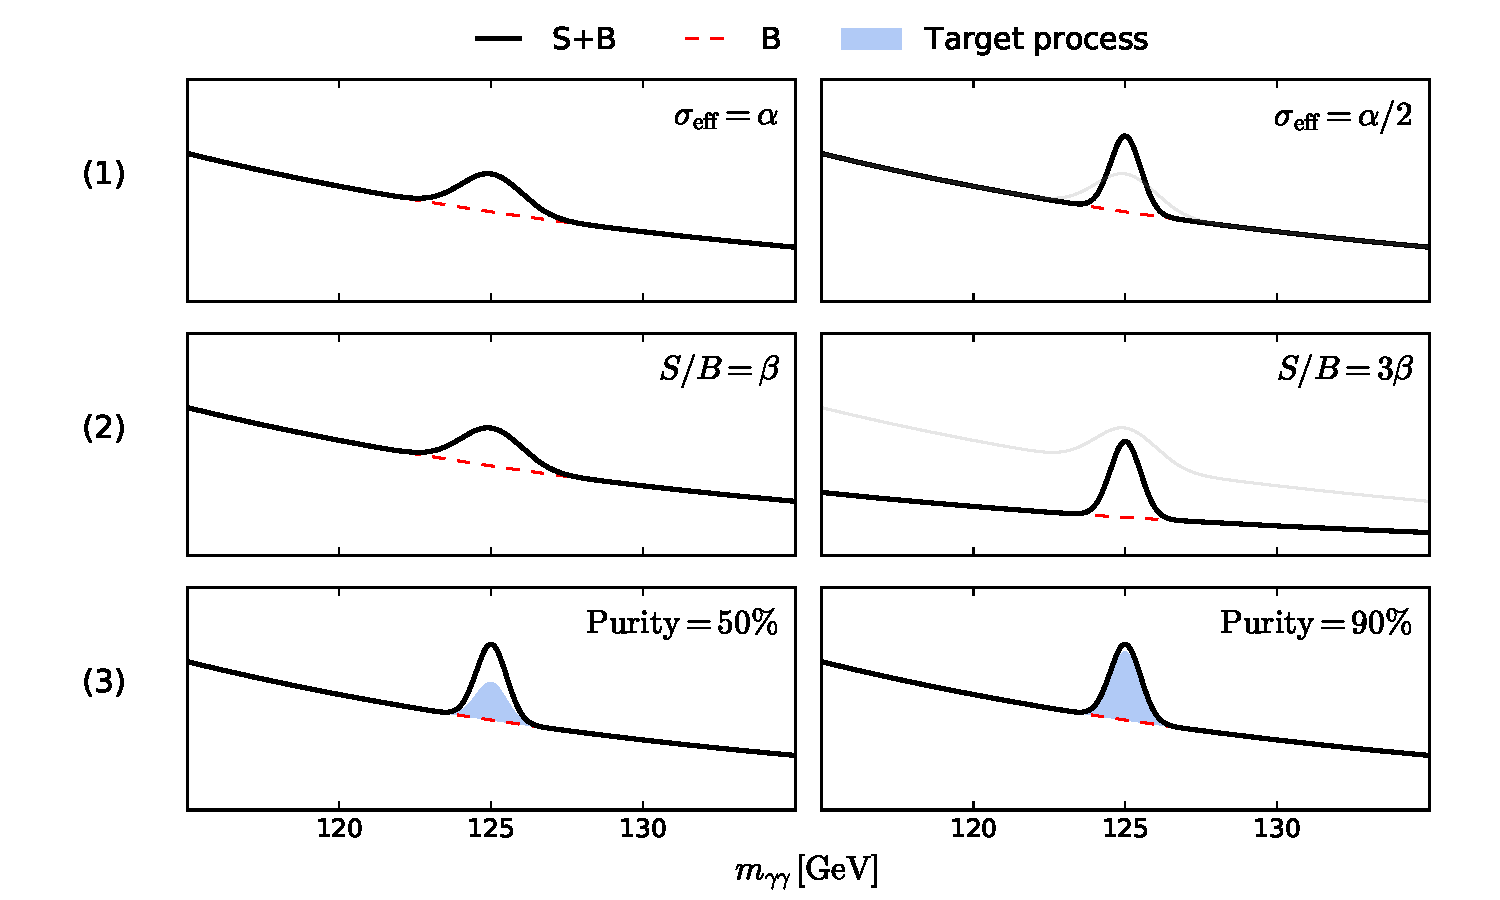
\includegraphics[width=1\textwidth]{Figures/hgg_overview/hgg_improve_measurement.pdf}
  \caption[Avenues for improving \Hgg measurements.]
  {
    An illustration of the various means of improving the measurements of Higgs boson properties in the diphoton decay channel. The top row demonstrates the effect of improving the diphoton mass resolution, leading to a narrower signal peak. The middle row shows the effect of improving the signal-to-background ratio, which would result from using a more powerful signal-vs-background discriminator. Finally, the bottom row represents the improvement from increasing the target signal process purity.
  }
  \label{fig:hgg_overview_improving_measurements}
\end{figure}

\begin{enumerate}
    \item The diphoton mass resolution: a narrower signal peak is more easily distinguished from the background continuum and therefore results in an enhanced sensitivity. The diphoton mass resolution is driven by the energy response of the ECAL (see Section~\ref{sec:cms_ecal}). A good mass resolution also relies on the correct identification of photons from other objects in the detector such as jets. Furthermore, the precise assertion of the interaction vertex from which the two photons originate is crucial for accurately determining the opening angle, $\theta$.
    
    \item The signal-to-background ratio in an analysis category: the sensitivity is improved by reducing the background contamination under the Higgs boson peak. In this analysis, ML algorithms are used to better discriminate between signal and background. Since different background processes are important for different Higgs boson production modes, a number of signal-vs-background classifiers are trained and used in the relevant analysis categories.
    
    \item The purity of the signal events in an analysis category: here, analysis categories are defined to target specific bins of the STXS framework. Therefore to improve the sensitivity, we aim to maximise the purity of an analysis category with respect to the targeted STXS bin (or bins). In other words, make the confusion matrix which quantifies the fraction of each truth-level STXS bin in each reconstruction-level event category as diagonal as possible (see Figure~\ref{fig:purity_matrix}). This helps the unfolding procedure, and reduces the correlations between the measured cross sections.
\end{enumerate}

This chapter will focus on the experimental techniques used to maximise the sensitivity of the analysis, according to the three aspects stated above. Several applications of ML algorithms are introduced, to perform both regression and classification tasks. Appendix~\ref{app:ML} provides an introduction to the foundations of ML, and will help the reader familiarise themselves with a number of recurrent concepts. Firstly, the data and MC simulation samples used in the analysis are introduced. Section \ref{sec:event_reconstruction} then details the procedure used to reconstruct candidate \Hgg events, specifically the techniques which improve the diphoton mass resolution: the additional photon energy corrections, the photon identification and selection, and the primary vertex selection. Following this, the reconstruction-level categorisation of events is described in Section~\ref{sec:event_categorisation}. Additional objects in the events such as jets and charged leptons, and quantities such as the missing transverse momentum are used to define categories targeting the different truth-level STXS bins. This section covers the methods used to both reduce background contamination and to increase the purity of the targeted STXS bin (or bins) in such categories\footnote{For clarity, throughout the following three chapters the terms ``analysis category" or ``tag" refer to the \textit{reconstruction-level} event categories that are constructed for this analysis. On the other hand, the term ``STXS bin" refers to a kinematic region of phase-space defined at \textit{truth-level}. It is the STXS bin cross sections that the analysis aims to measure.}.

%%%%%%%%%%%%%%%%%%%%%%%%%%%%%%%%%%%%%%%%%%%%%%%%%%%%%%%%%%%%%%%%%%%%%%%%%%%%%%%%%%%%%%%%%%%%%%%%%

\section{Samples}
\subsection{Data}
This analysis uses p-p collision data collected by the CMS experiment at $\sqrt{s}$~=~13~TeV during Run 2 of the LHC. The total integrated luminosity is 137~\fbinv, of which 35.9~\fbinv was collected in 2016, 41.5~\fbinv in 2017 and 59.4~\fbinv in 2018.

% Events in data are selected using the two-tiered trigger system described in section \ref{sec:trigger}. A seed at the L1T stage is defined as a deposit of energy in the ECAL, above a certain energy threshold, which is subsequently passed to the HLT path. Despite signal events being characterised by two photon candidates, a higher overall efficiency is achieved if only one seed is required at the L1T stage, with a tight transverse energy threshold applied to the seed in order to limit the rate of events passing to a manageable level. The energy threshold is typically set at 40~GeV, lowering to 30-32~GeV for isolated L1T seeds in the ECAL. With the presence of this energy threshold, there is an unavoidable drop in efficiency for \Hgg events at low transverse energy. To circumvent this effect, an additional double-seed selection is included at the L1T with lower energy thresholds than the single-seed trigger. In 2016, the thresholds were set to 23 and 10~GeV for the leading and subleading seeds respectively, rising to 25 and 14~GeV for the 2017 and 2018 data taking periods.

% At the HLT, a basic version of the offline clustering algorithm, described in section \ref{sec:particle_flow}, is applied to the energy deposits in the ECAL. Here, events are required to contain two SCs with invariant mass greater than 90~GeV and passing asymmetric $p_T$ thresholds, initially set at 30 and 18~GeV. After the 2016 data-taking period, the lower threshold was raised to 22~GeV to counterbalance the increased instantaneous luminosity and hence maintain a constant event rate. In addition, a number of selection criteria are imposed on higher-level variables related to the SC shower-shape, isolation and the ratio of the HCAL and ECAL deposits. Events passing the HLT selection then enter the \Hgg analysis.

Events in data are selected using the two-tiered trigger system described in Section \ref{sec:trigger}. The tag-and-probe method is used to evaluate the efficiency of the trigger selection~\cite{CMS:2011aa}. This method exploits the decay of a known resonance such as the Z boson, where the \textit{tag} is defined as one of the decay products passing very tight identification criteria, and the \textit{probe} as the other decay product, subject to much looser identification requirements. Moreover, the combined invariant mass of the tag-and-probe pair is required to be consistent with the mass of the original resonance to ensure a high purity sample. For some selection criteria, $\mathcal{C}$, the efficiency, $\epsilon_{\mathcal{C}}$, is then defined as the fraction of probes passing $\mathcal{C}$. This method remains valid as long as the identification requirements on the probe do not affect the efficiency of $\mathcal{C}$.

Given the proximity of the Z boson and Higgs boson masses, as well as the fact that both electrons and photons are reconstructed as SCs in the ECAL, \Zee events in data provide an excellent candidate for evaluating efficiencies in the \Hgg analysis. Dielectrons with invariant mass close to the Z boson mass are used to define the tag and probe. After reweighting the \Zee events to match the $\eta$ and $R_9$ (see Section~\ref{sec:photon_preselection}) distributions of \Hgg events, the trigger efficiency is evaluated per SC in bins of the probe electron $p_T$, $\eta$ and $R_9$. For an SC in the EB and EE, the average trigger efficiencies are above 97\% and 95\%, respectively. The product of the two per-SC efficiencies of the diphoton is then used to weight simulated events to replicate the trigger efficiency observed in data.  Ultimately, the trigger selection criteria are significantly looser than the offline selection criteria applied in the \Hgg analysis, ensuring that the trigger has a negligible effect on the \Hgg selection efficiency.

%Ultimately, since the analysis selection thresholds are much tighter than those of the trigger, the per-event trigger efficiency is greater than 99\% with respect to the analysis selection.

\subsection{Simulation}\label{sec:hgg_simulation}
Monte Carlo (MC) simulated events are used for both training event classifiers and constructing the final signal model. The simulated events are subject to the exact same event reconstruction and categorisation procedure as used for data. 

Signal samples were simulated for the different Higgs boson production mechanisms at next-to-leading order (NLO) in perturbative QCD using the \textsc{MG5\_aMC@NLO} (version~2.4.2)~\cite{Alwall:2014hca}, and \textsc{Powheg} (version~2.0) generators~\cite{Nason:2004rx,Frixione:2007vw,Alioli:2008tz,Nason:2009ai,Alioli:2010xd,Hartanto:2015uka}. When possible, an independent event sample from the alternative generator is used for training event classifiers, thus ensuring the event categorisation and the construction of the final signal model are independent. Events produced via ggH production are weighted as a function of the Higgs boson $p_T$ and the number of jets to match the predictions of the NNLOPS program~\cite{Hamilton:2013fea}. Parton distribution functions (PDFs) used to model the distribution of colliding partons inside the initial-state protons are taken from the NNPDF 3.0 (NNPDF~3.1) set~\cite{Ball:2014uwa,Ball:2017nwa}, when simulating 2016 (2017/2018) data. The parton-level events are subsequently interfaced with \textsc{Pythia8} (version 8.226 for 2016 MC and version 8.230 for 2017/2018 MC) for decaying the Higgs boson to photons, parton showering and hadronisation~\cite{Sjostrand:2014zea}. The \textsc{Pythia8} CUETP8M1~\cite{Khachatryan:2015pea} and CP5~\cite{Sirunyan:2019dfx} tunes are used for the simulation of 2016 data and 2017/2018 data, respectively.

The signal samples are normalised according to the production cross sections and the \Hgg branching fraction (0.227\%) recommendations by the LHCHWG~\cite{deFlorian:2016spz}. The fractional breakdown of each production mode in the STXS bins is computed directly from the signal MC samples, and serves as the SM prediction of the cross section in each bin. Table \ref{tab:signal_samples} summarises the event generators used for the signal simulation, as well as the total cross section times branching fraction, $\sigma_{\text{SM}}\mathcal{B}$, for each production mode with details on the order of the calculation. The fractional breakdowns of each production mode into the STXS bins are shown in Chapter \ref{chap:theory} in Tables~\ref{tab:ggH_definitions}--\ref{tab:top_definitions}.

\begin{table}[t]
    \caption[Signal simulation details]{Details of the signal simulation. For each production mode, the generator used for the final signal-modelling is listed. If available, an independent sample is used from the alternative generator when training the event classifiers. In addition, the cross sections times branching fraction, $\sigma_{\text{SM}}\mathcal{B}$, are provided for a nominal Higgs boson mass, $m_{\rm{H}}=125.0$~GeV, at $\sqrt{s}~=~13$~TeV. The final column details the order of the cross section calculation. For the tHq, tHW and bbH production modes, the flavour scheme (FS) used in the calculation is specified, where 5FS (4FS) includes (does not include) the bottom quark/anti-quark components in the colliding protons.}
    \label{tab:signal_samples}
    % \vspace{.5cm}
    \centering
    \scriptsize
    \hspace*{-5cm}
    \renewcommand{\arraystretch}{2}
    \setlength{\tabcolsep}{5pt}
    \begin{tabular}{lcccc}
    \hline
   Production mechanism & Naming convention & Generator & $\sigma_{\text{SM}}\mathcal{B}$~[fb] & Order of $\sigma_{\rm{SM}}$ calc \\ \hline
   ggH & ggH & \textsc{MG5\_aMC@NLO} & 110.27 & N$^{\rm{3}}$LO(QCD)+NLO(EW) \\
   gg$\rightarrow$ZH, Z$\rightarrow$qq & ggZH had & \textsc{Powheg} & 0.19 & NNLO(QCD)+NLO(EW) \\
   \hline
   VBF & VBF & \textsc{MG5\_aMC@NLO} & 8.59 & NNLO(QCD)+NLO(EW) \\
   qq/qg$\rightarrow$WH, W$\rightarrow$qq & WH had & \textsc{MG5\_aMC@NLO} & 2.10 & NNLO(QCD)+NLO(EW) \\
   qq/qg$\rightarrow$ZH, Z$\rightarrow$qq & ZH had & \textsc{MG5\_aMC@NLO} & 1.40 & NNLO(QCD)+NLO(EW) \\
   \hline
   qq/qg$\rightarrow$WH, W$\rightarrow\ell\nu$ & WH lep & \textsc{MG5\_aMC@NLO} & 1.016 & NNLO(QCD)+NLO(EW) \\
   qq/qg$\rightarrow$ZH, Z$\rightarrow\ell\ell/\nu\nu$ & ZH lep & \textsc{MG5\_aMC@NLO} & 0.520 & NNLO(QCD)+NLO(EW) \\
   gg$\rightarrow$ZH, Z$\rightarrow\ell\ell/\nu\nu$ & ggZH lep & \textsc{Powheg} & 0.084 & NNLO(QCD)+NLO(EW) \\
   \hline
   ttH & ttH & \textsc{MG5\_aMC@NLO} & 1.155 & NLO(QCD)+NLO(EW) \\
   \hline
   tHq & tHq & \textsc{MG5\_aMC@NLO} & 0.175 & NLO(QCD) in 5FS \\
   tHW & tHW & \textsc{MG5\_aMC@NLO} & 0.034 & NLO(QCD) in 5FS \\
   \hline
   bbH & bbH & \textsc{MG5\_aMC@NLO} & 1.108 & NNLO(5FS)+NLO(4FS) \\
   \hline

\end{tabular}
    \hspace*{-5cm}
\end{table}

The final background model used for the extraction of results is derived directly from data. Nevertheless, simulated background events are required for training the multivariate event classifiers. For inclusive production, the dominant source of background is SM diphoton production, which is simulated using the \textsc{Sherpa} (version 2.2.4) generator~\cite{Gleisberg:2008ta}. In this sample, matrix elements are calculated at NLO and LO for up to one and three additional partons, respectively, which are subsequently matched with the \textsc{Sherpa} generator parton showering. A subdominant background originates from $\gamma$+jet or jet+jet events, where the jets are misidentified by the PF algorithm as isolated photons. These backgrounds are simulated with \textsc{Pythia8}, applying a filter in the generation to enrich the production of jets with high electromagnetic activity. Furthermore, other sources of background become important for categories targeting the sub-dominant production modes, such as diboson production in the VH leptonic categories and tt+$\gamma\gamma$ in the top-associated categories. Additional MC samples simulated with the \textsc{MG5\_aMC@NLO} and \textsc{Powheg} generators are used to model such backgrounds. Finally, Drell-Yan events with leptonic final-states and tt+Z events are used for validation purposes. Both are simulated with the \textsc{MG5\_aMC@NLO} generator and \textsc{Pythia8} for parton showering and hadronisation.

Each particle-level sample is propagated through the \textsc{Geant4} package to model the response of the CMS detector~\cite{Agostinelli:2002hh}. Separate MC samples are produced for each year to account for the variations in the detector conditions and the LHC beam parameters. This modelling includes the effect of pileup interactions originating from both the nominal bunch-crossing (in-time pileup) and the crossing of previous and subsequent proton bunches (out-of-time pileup). The simulation is weighted to match the distribution of the number of interaction vertices in data, which corresponds to an average pileup of 23 in 2016, and 32 in 2017 and 2018.

%%%%%%%%%%%%%%%%%%%%%%%%%%%%%%%%%%%%%%%%%%%%%%%%%%%%%%%%%%%%%%%%%%%%%%%%%%%%%%%%%%%%%%%%%%%%%%%%%
% \newpage
\section{Event reconstruction}\label{sec:event_reconstruction}
This section describes the offline reconstruction of events passing the trigger selection. The data and the corresponding simulation are reconstructed separately for each year to account for the differences in the detector performance and LHC beam parameters. 

\subsection{Photon reconstruction}\label{sec:photon_reconstruction}
Photons are defined using the set of photon candidates from the PF algorithm (see Section \ref{sec:particle_flow}). In the algorithm, SCs are formed by clustering together deposits of energy in the ECAL crystals, consistent with originating from the same electromagnetic shower. Due to imperfect shower containment in the crystals and shower losses for photons which convert to \ee pairs before reaching the ECAL, the SC energy, \Eraw, can often differ from the true initial photon energy, \Etrue. As described in Section~\ref{sec:cms_ecal}, a multivariate regression technique is applied to all photons to correct for such losses, estimating both the value of \Etrue and its uncertainty. Remaining differences in the photon-energy scale and resolution between data and simulation are accounted for using a series of additional scale and smearing corrections, derived using \Zee events. Photons are then subject to a set of selection criteria (pre-selection) concerning the photon shower-shape, kinematic, and isolation variables. In addition, a ML algorithm known as a Boosted Decision Tree (BDT, see Appendix~\ref{app:ML}) is trained to separate genuine photons from fake photons; this is referred to as the photon-identification BDT. The selection includes a minimum requirement on the output score of this BDT, which reduces the contribution from background processes with hadronic jets mimicking a photon signature. Before describing the photon reconstruction techniques in more detail, it is useful to list the photon variables used in the \Hgg analysis in Table~\ref{tab:photon_variables}. Two of these variables, namely \RNINE and $\mathcal{I}_{\rm{ph}}$, are shown in Figure~\ref{fig:photon_id_0} when describing the photon-identification BDT. The distributions correspond to probe electrons from \Zee decays, however the photon distributions are effectively the same since photons and electrons have almost identical shower profiles in the ECAL.

\begin{table}
    \caption[Photon variables]{A summary of the photon variables used in this analysis. The shower-shape variables are used to both correct the photon energy in the regressor (see Section~\ref{sec:cms_ecal}) and to discriminate between real and fake photons. The isolation variables help to identify real photons from other objects such as jets mimicking a photon signature.}
    \label{tab:photon_variables}
    % \vspace{.5cm}
    \centering
    \scriptsize
    \renewcommand{\arraystretch}{2}
    \hspace*{-1.5cm}
    \begin{tabular}{r|p{0.85\textwidth}}
    \multicolumn{2}{c}{\textbf{Shower shape variables}} \\ \hline
    $\RNINE$ & (=$E_{3\times3}/\Eraw$) The ratio of the energy sum in the $3\times3$ grid surrounding the SC seed to the energy of the SC before corrections. The value of \RNINE is typically high ($>0.85$) for unconverted photons, and typically lower ($<0.85$) for photons that have undergone a conversion upstream of the ECAL. \\
    $E_{2\times2}/E_{5\times5}$ & The ratio of the energy sum in the $2\times2$ grid containing the most energetic crystals in the SC, to the energy in the $5\times5$ grid surrounding the SC seed. \\
    $\sigma_{\eta}$ & A measure of the lateral extension of the shower, defined as the standard deviation of single crystal $\eta$ values within the SC, weighted by the logarithm of the crystal energy. \\
    $\sigma_{i\eta i\eta}$ & The standard deviation of the shower in $\eta$ in terms of the absolute number of crystal cells. \\
    $\sigma_{\phi}$ & A measure of the lateral extension of the shower, defined as the standard deviation of single crystal $\phi$ values within the SC, weighted by the logarithm of the crystal energy.  \\
    ${\rm{cov}}_{i\eta i\phi}$ & The covariance of the single crystal $\eta$ and $\phi$ values for the $5\times5$ grid centred around the crystal with the most energy.  \\
    $\sigma_{RR}$ & For photons in the ECAl endcaps only, the standard deviation of the shower spread in the x-y plane of the preshower detector. \\
    $n_{\rm{clusters}}$ & The number of clusters in the SC. \\
    \hline
    \multicolumn{2}{c}{\textbf{Isolation variables}} \\ \hline
    $H/\Eraw$ & Ratio of the energy in the HCAL cells directly behind the SC to the energy of the SC. \\
    $\mathcal{I}_{\rm{ph}}$ & Photon isolation, defined as the sum of transverse energy of PF photons falling inside a cone of radius ${\Delta}R=\sqrt{\Delta\eta^2+\Delta\phi^2}=0.3$ around the SC. The transverse energies are corrected using $\rho$ to mitigate the effect of pileup. \\
    $\mathcal{I}_{\rm{ch}}$ & Charged hadron isolation, defined as the sum of transverse energy of the PF charged hadrons falling inside a cone of radius ${\Delta}R=0.3$ around the SC. This is measured with respect to both the selected and the worst vertex; the benefit of this is that true photons are generally isolated from other vertices, but fake photons are not. \\
    $\mathcal{I}_{\rm{tk}}$ & Track isolation, defined as the sum of transverse energy of all tracks in a hollow cone with a smaller (larger) annulus of ${\Delta}R=0.04$ (${\Delta}R=0.3$). \\
    \hline
    \multicolumn{2}{c}{\textbf{Other variables}} \\ \hline  
    Electron veto & Boolean flag variable which is set to false if the supercluster is matched to an electron track. \\
    $\rho$ & Median energy density per unit area in the event (sensitive to pileup). \\
    \Eraw & Uncorrected supercluster energy. \\
    \Etrue & True photon energy. \\
\end{tabular}
    \hspace*{-1.5cm}
\end{table}

\subsubsection{Photon energy}
% The photon energy response of the ECAL (\Etrue/\Eraw) is parameterised by a function with a Gaussian core and power law tails. Using simulated photons, a multivariate regressor is trained to estimate the shape parameters of this energy response function, thus providing a prediction of the full \Etrue/\Eraw probability density function for each photon~\cite{Khachatryan:2015iwa}. The mode of this predicted function is used to correct \Eraw to \Etrue, whilst the shape provides a per-photon-energy resolution estimate used later in the event categorisation (section \ref{sec:event_categorisation}).

% The regressor corrects not only for the imperfect shower containment arising from converting photons and electromagnetic showers that begin upstream of the ECAL, but also for the localised containment within the ECAL, where energy can be lost in the gaps between crystals. Input variables related to the SC shower-shape provide information on the upstream showering and photon conversions, which combined with the SC $\eta$ and $\phi$ values allows the regressor to learn variations in the ECAL geometry. On the other hand, the seed crystal positions and seed cluster energy ratios enable the regressor to correct for the localised containment effects. In addition, the total number of primary vertices and the total energy density, $\rho$, are included to account for systematic enhancements of \Eraw due to pileup.

After applying the photon energy regression described in Section~\ref{sec:cms_ecal}, a number of residual discrepancies between data and simulation remain that cannot be derived from simulation alone. Using \Zee events in data, in which the electrons are reconstructed as photons\footnote{Meaning no track information is used in the reconstruction, and the energy is determined using the algorithm and corrections corresponding to photons rather than electrons.}, a series of scale and smearing corrections are derived to correct the photon-energy scale and resolution~\cite{Sirunyan:2020xwk}. To account for the degradation of the ECAL crystal performance over time, and the subsequent drift in energy scale this causes, a time-dependent correction is applied in bins which equate roughly to the duration of one LHC fill. This ensures the energy scale of the ECAL is constant over time. Subsequently, the dielectron mass spectrum, $m_{ee}$, is used to simultaneously shift the peak in data to match that in simulation, and smear the resolution in simulation to match that in data. These scale and smearing corrections are applied differentially in bins of SC $\eta$ and \RNINE. 

\begin{figure}
  \centering
  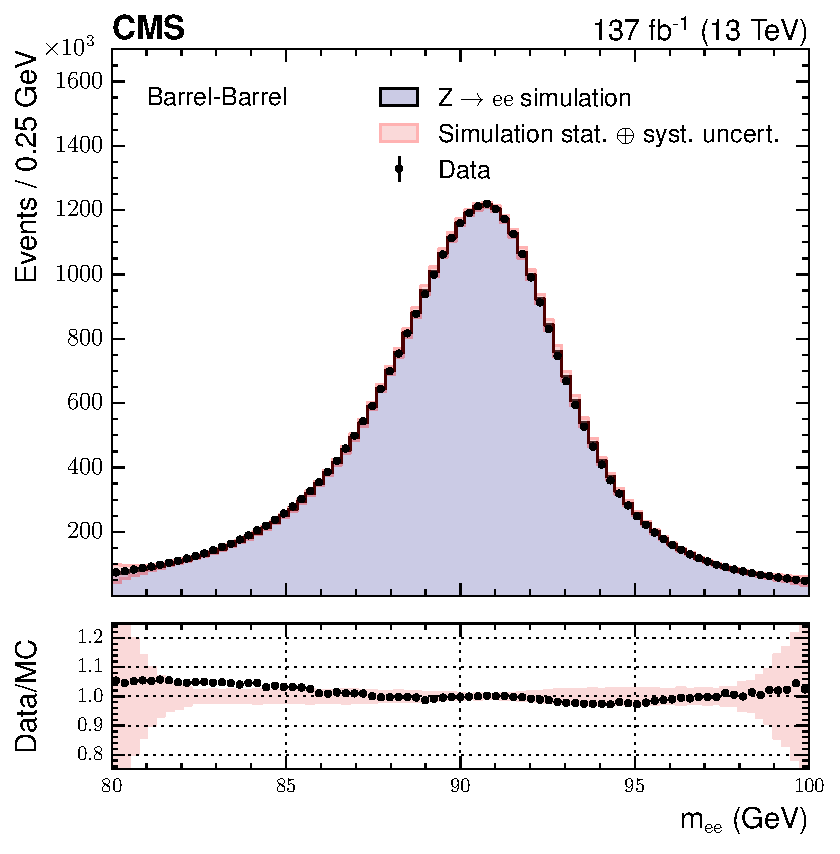
\includegraphics[width=.49\textwidth]{Figures/hgg_overview/money_run2_EbEb_inclusive.pdf}
  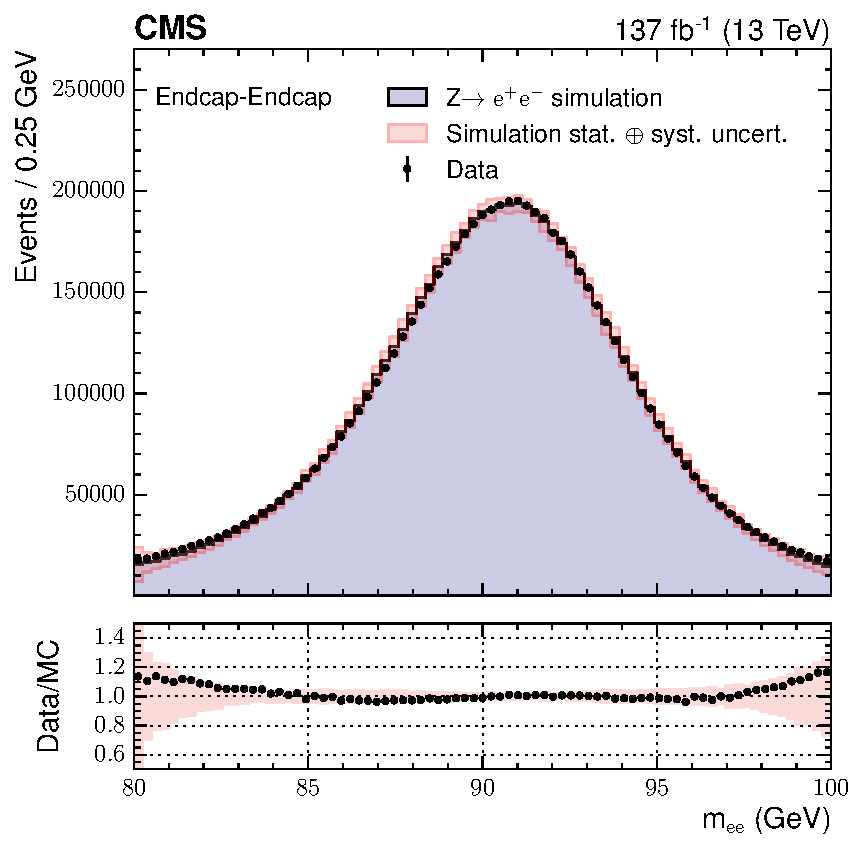
\includegraphics[width=.49\textwidth]{Figures/hgg_overview/money_run2_EeEe_inclusive.pdf}
  \caption[Dielectron mass spectrum for \Zee events in data and simulation after the energy corrections are applied]
  {
    Comparison of the dielectron mass spectrum for \Zee events in data (black points) and simulation (filled histogram), after the full set of energy scale and smearing corrections are applied. The total uncertainty in the simulated events is shown by the pink bands. The plots show the full data set collected during the 2016-2018 data-taking period, and the corresponding simulation, where the left-hand (right-hand) plot corresponds to events in which both electrons are reconstructed in the ECAL barrel (endcaps).
  }
  \label{fig:photon_energy_0}
\end{figure}

Referring back to equation \ref{eq:mgg}, all techniques\footnote{Including the energy corrections described in Section~\ref{sec:cms_ecal}.} used to improve the photon-energy resolution, $\sigma_E/E$, in turn improve the diphoton mass resolution, $\sigma_m/m_{\gamma\gamma}$, and thus lead to an enhanced sensitivity to Higgs boson production. Figure \ref{fig:photon_energy_0} shows the $m_{ee}$ distributions for \Zee events in both data and simulation, after the full set of energy corrections are applied. The left-hand panel shows the situation where both electrons are reconstructed in the ECAL barrel, and the right-hand panel where both are reconstructed in the ECAL endcaps. The pink bands indicate the statistical and systematic uncertainty in the simulation, where the systematic component includes contributions which are related to the measurement and reconstruction of the photon energy (see Section~\ref{sec:systematics}). Clearly, after the corrections are applied, the data and simulation are in good agreement, within the uncertainty bands.



\subsubsection{Photon pre-selection}\label{sec:photon_preselection}
Table \ref{tab:photon_preselection} provides a schema of the selection criteria applied to the photon candidates. The pre-selection efficiency is calculated using the tag-and-probe method on \Zee events for all selection criteria, barring the requirement on the electron veto, which is computed using \Zmumug events. For the latter, the $\mu^{+}\mu^{-}\gamma$ system is required to be consistent with the decay of a Z boson, with a three-body invariant mass between 60 and 120~GeV. Probes are then defined as the set of photons passing all pre-selection criteria except the electron veto, and the efficiency is simply calculated as the fraction of these probes which pass the veto. The total pre-selection efficiency is computed for both data and simulation in bins of photon $\eta$ and \RNINE, and is typically above 95\% for photons with high values of \RNINE ($>0.85$) and around 90\% for photons with lower \RNINE ($<0.85$). Weights are then applied differentially per photon to match the pre-selection efficiencies in simulation to those observed in data.

\begin{table}[t]
    \caption[Schema of the photon pre-selection criteria]{Schema of the photon pre-selection criteria. The shower-shape and isolation requirements are different for photons in the ECAL barrel and for photons in the ECAL endcaps. These are then split into regions of different \RNINE criteria, with varying levels of additional selection on $\sigma_{i\eta i\eta}$, $\mathcal{I}_{\rm{ph}}$ and $\mathcal{I}_{\rm{tk}}$.}
    \label{tab:photon_preselection}
    \vspace{.5cm}
    \centering
    \scriptsize
    \renewcommand{\arraystretch}{1.8}
        \begin{tabular}{p{0.25\textwidth}|p{0.7\textwidth}}
       Minimum \pt  & $p_T^{\gamma 1}>35$~GeV (leading), $p_T^{\gamma 2}>25$~GeV (subleading) \\
       $\downarrow$ & \\
       Geometrical acceptance & $|\eta| < 2.5$, excluding barrel-endcap transition region $1.44 < |\eta| < 1.57$ \\
       $\downarrow$ & \\
       Electron veto & True \\
       $\downarrow$ & \\
       Hadronic shower rejection & H/\Eraw~$<0.08$ \\
       $\downarrow$ & \\
       Shower shape and isolation requirements
       & For photons in the EB:
       \begin{tabular}{c|ccc}
            \RNINE & $\sigma_{i\eta i\eta}$ & $\mathcal{I}_{\rm{ph}}$ (GeV) & $\mathcal{I}_{\rm{tk}}$ (GeV) \\ \hline
            $>0.85$ & - & - & - \\
            $[0.50,0.85]$ & $<0.015$ & $<4.0$ & $<6.0$ \\
       \end{tabular} \\
       & \\
       & For photons in the EE:
       \begin{tabular}{c|ccc}
            \RNINE & $\sigma_{i\eta i\eta}$ & $\mathcal{I}_{\rm{ph}}$ (GeV) & $\mathcal{I}_{\rm{tk}}$ (GeV) \\ \hline
            $>0.90$ & - & - & - \\
            $[0.80,0.90]$ & $<0.035$ & $<4.0$ & $<6.0$ \\
       \end{tabular} \\
       & \\
       & All photons: (\RNINE$>0.8$ and $\mathcal{I}_{\rm{ch}}<20$~GeV) or ($\mathcal{I}_{\rm{ch}}/p_T^{\gamma}<0.3$)

    \end{tabular}
\end{table}


\subsubsection{Photon identification}
The photon-identification (photon-ID) BDT aims to distinguish between real photons in the CMS detector and hadronic jets mimicking a photon signature. The BDT is trained using the $\gamma$+jet simulation sample, where the true photon is used as signal and the fake photon from the jet as background. Photon shower-shape, kinematic, and isolation variables are used as input features to the BDT, along with parameters sensitive to pileup, such as the median-energy-density per unit area, $\rho$. 

One of the dominant sources of systematic uncertainty in the \Hgg analysis arises from the modelling of the electromagnetic shower in simulation, in particular the variables describing the shower-shape and isolation. Since these variables are direct inputs to the photon-ID BDT, any discrepancies between data and simulation are propagated to the output BDT score, and thus introduce a systematic uncertainty into the analysis. To mitigate this, a chained quantile regression (CQR) method~\cite{CQR} is applied, which sequentially corrects the photon-ID BDT input variables in simulation. 

The corrections are derived using a set of probe electrons in \Zee events. The CQR method morphs the distribution of some photon-ID BDT input variable, $y_i$ (e.g. \RNINE), in simulation to match that in data by training a series of 21 BDTs to predict points along the cumulative distribution function, CDF($y_i$): [0.01,0.05,0.10,...,0.95,0.99]. For example, the CQR BDTs predict the values of \RNINE at which the CDF(\RNINE) is equal to the 21 points ranging from 0.01 to 0.99. The full CDF is determined by linearly interpolating between these 21 points, and is extracted separately for both data and simulation. A correction is then applied to the simulated variable, per electron, according to:
\begin{equation}
    y_i \longrightarrow y_i^{\rm{corr}} = {\rm{CDF}}^{-1}_{\rm{data}}({\rm{CDF}}_{\rm{simulation}}(y_i)),
\end{equation}
\noindent 
which successfully morphs the distribution of $y_i$ in simulation to match that in data. 

Shower-shape variables are first ordered into a chain: [$S_1$,$S_2$,...$S_N$]. The CDF for the first variable, $S_1$, is predicted using solely the electron $p_T$, $\eta$, $\phi$ and global energy density, $\rho$, as input features to the 21 BDTs. For variable, $S_i$, the input features also include the previously processed shower-shape variables: [$S^{\rm{corr}}_1$,...,$S^{\rm{corr}}_{i-1}$] for simulation and [$S_1$,...,$S_{i-1}$] for data. By deriving the corrections in this manner, correlations between the photon-ID BDT input variables are accounted for. The ordering of the chain is optimised to minimise the final discrepancy between data and simulation in the photon-ID BDT output score. For example, the shower-shape variables are corrected in 2018 simulation according to the chain ordering,

\begin{equation}
    \big[\,{\rm{cov}}_{i\eta i\phi},\, E_{2\times2}/E_{5\times5},\, \RNINE,\, \sigma_{\phi},\, \sigma_{i\eta i\eta},\, \sigma_\phi\,\big].
\end{equation}

For isolation variables, $\mathcal{I}_i$, an additional stochastic-shifting procedure is applied to account for electrons migrating across the discontinuity in the distributions i.e. from the peak at $\mathcal{I}_i=0$, to the tail at $\mathcal{I}_i>0$. Two additional classifiers are trained to predict the probabilities for electrons to fall in the peak or tail, given the electron $p_T$, $\eta$ and $\phi$, and the energy density, $\rho$. Using the output probabilities, the simulated electrons are then migrated between the peak and tail to match the relative compositions in data. Finally, the distribution of electrons in the tail is then corrected using the quantile morphing technique described above. Figure \ref{fig:photon_id_0} demonstrates the performance of the CQR method for shower-shape variable, \RNINE (left) and isolation variable, $\mathcal{I}_{\rm{ph}}$ (right).

\begin{figure}
  \centering
  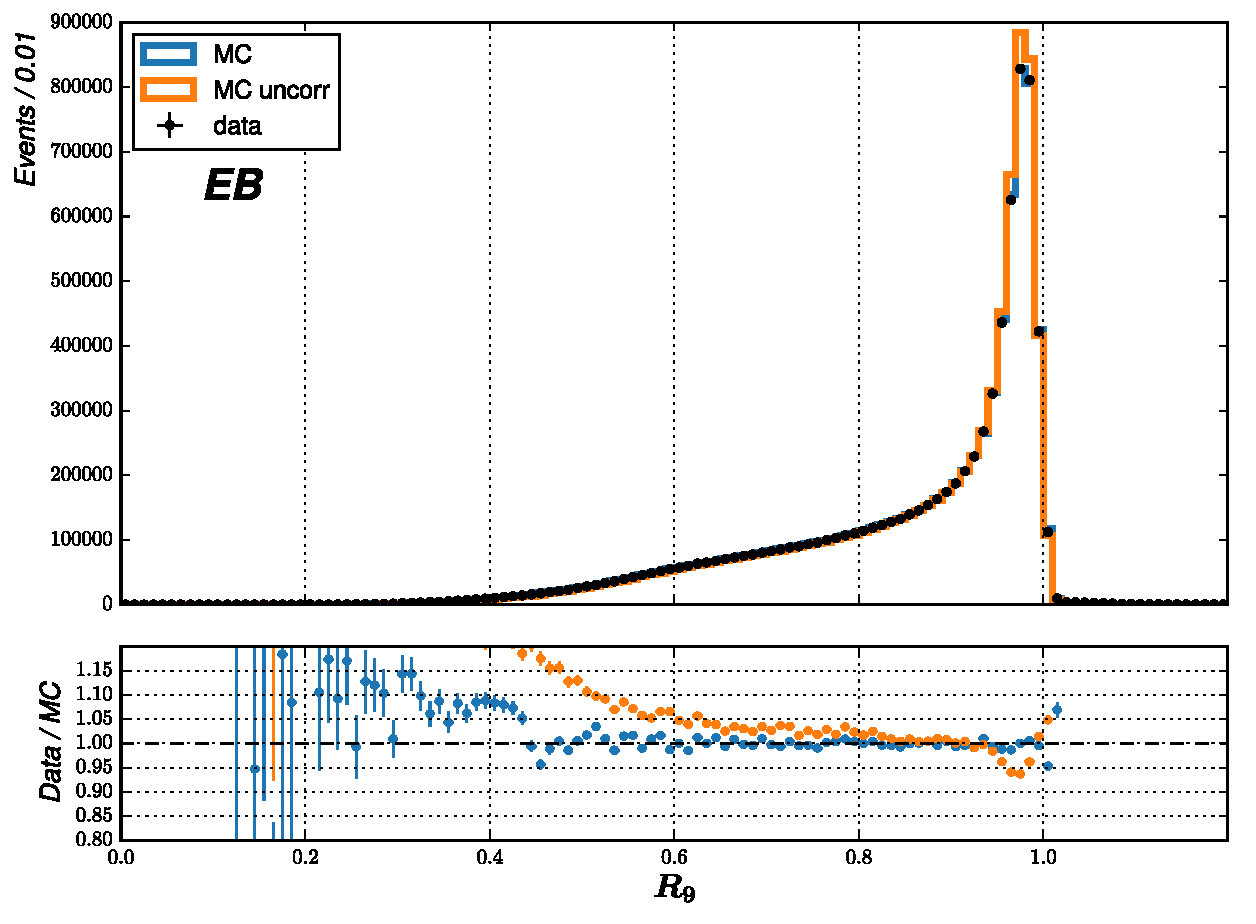
\includegraphics[width=.49\textwidth]{Figures/hgg_overview/dataMC_probeR9_0_corr.pdf}
  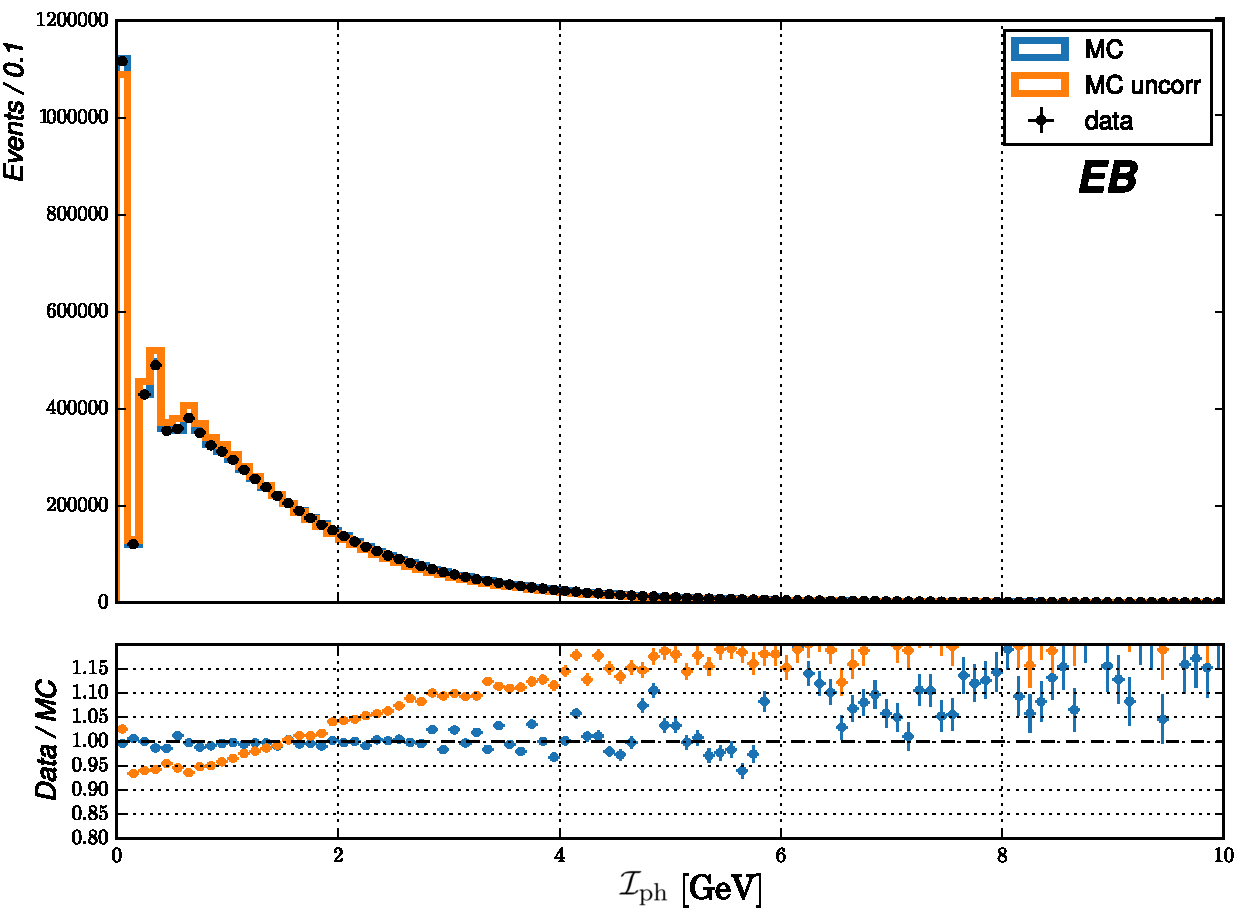
\includegraphics[width=.49\textwidth]{Figures/hgg_overview/dataMC_probePhoIso_0_corr.pdf}
  \caption[Corrections from the chained quantile regression method for \RNINE and $\mathcal{I}_{\rm{ph}}$]
  {
    Probe electron \RNINE (left) and $\mathcal{I}_{\rm{ph}}$ (right) distributions from \Zee events, where the probe electron is reconstructed in the ECAL barrel. The black points correspond to data taken in 2017. The corresponding simulation is shown without corrections in orange, and with the CQR corrections in blue. The bottom panel shows the ratio of data to simulation, clearly demonstrating the improved agreement after applying the CQR corrections.
  }
  \label{fig:photon_id_0}
\end{figure}

The systematic uncertainty originating from these corrections is derived by splitting the original \Zee samples in half, and re-calculating the corrections using the two independent event sets. The magnitude of the uncertainty is defined per-bin of the photon-ID BDT output score, as the standard deviation of the event-by-event corrected output score values. This assumes the major source of uncertainty in the method is originating from the limited size of the training samples. All in all, the CQR method provides a vastly improved technique for calculating the shower-shape and isolation corrections, reducing the impact of a dominant systematic uncertainty from around 5\% in previous \Hgg analyses to roughly 2\%.

The output score of the photon-ID BDT, for the lowest-scoring photon in the diphoton pair, is shown in Figure \ref{fig:photon_id_1}. The left-hand plot shows the distribution for signal and background processes, highlighting the impressive discriminating power between events with two real photons and the $\gamma$+jet and jet+jet backgrounds. The right-hand plot shows the same distribution for \Zee events in both data and simulation. The two are in excellent agreement, within the calculated uncertainties. For completeness, Figure~\ref{fig:photon_id_2} shows the photon-ID BDT score for probe electrons (\Zee) reconstructed in the EB, with and without the CQR corrections applied to the BDT input features. Clearly, the improved agreement between data and simulation in the input features propagates to the output score, thus demonstrating the power of the CQR method.

\begin{figure}
  \centering
  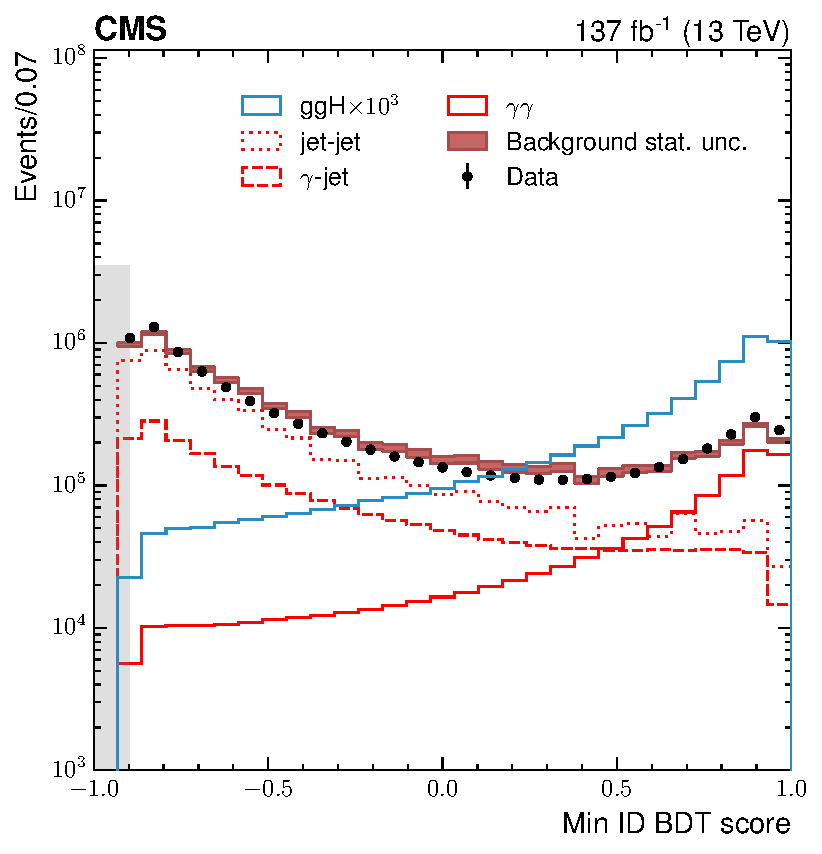
\includegraphics[width=.49\textwidth]{Figures/hgg_overview/DiphoBDT_minIDMVA_logPlot.pdf}
  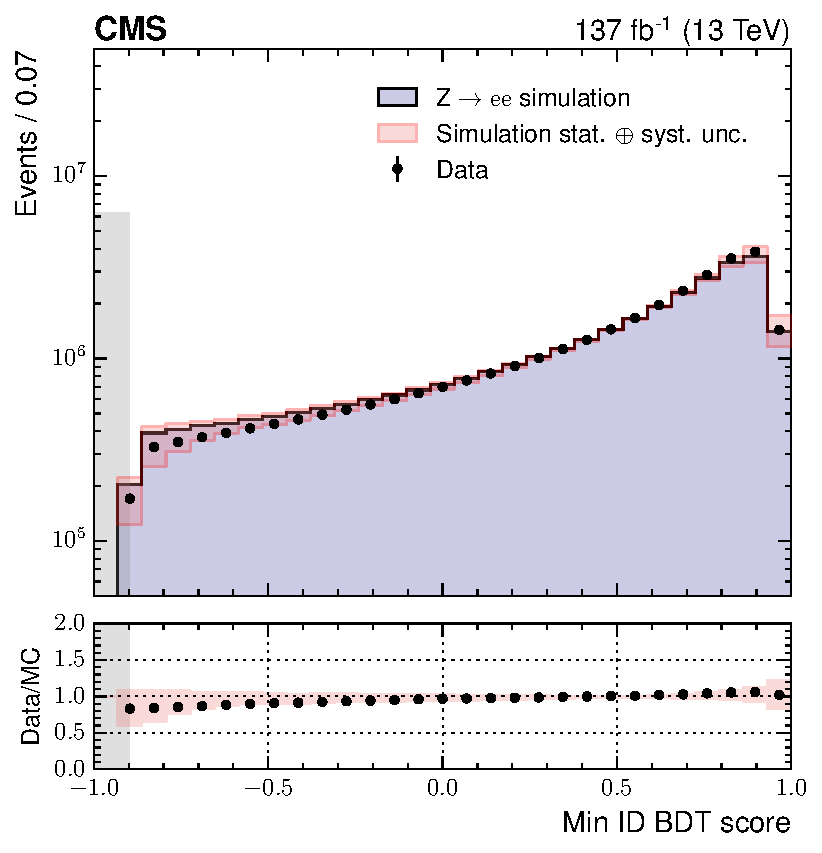
\includegraphics[width=.49\textwidth]{Figures/hgg_overview/DYValidation_DiphoBDT_RatioPlot_minIDMVA_logPlot.pdf}
  \caption[Photon ID output score distributions]
  {
    The left plot shows the distribution of the photon-ID BDT score of the lowest scoring photon in diphoton pairs with an invariant mass in the range ${100<\mgg<180}$~GeV. Data events passing pre-selection are shown by the black points. Simulated background events with the corresponding statistical uncertainty are shown by the pink band. The different components of the background and the Higgs boson signal events are also plotted, shown by the red and blue histograms respectively. The right plot shows the same distribution for \Zee events in data and simulation, where the electrons are reconstructed as photons. The total uncertainty in the simulation, calculated as the quadrature sum of the statistical and systematic components, is shown by the pink band. The shaded grey regions demonstrate the minimum threshold applied for photons in this analysis. The full data set collected in the period 2016-2018 and the corresponding simulation is shown.
  }
  \label{fig:photon_id_1}
\end{figure}

\begin{figure}
  \centering
  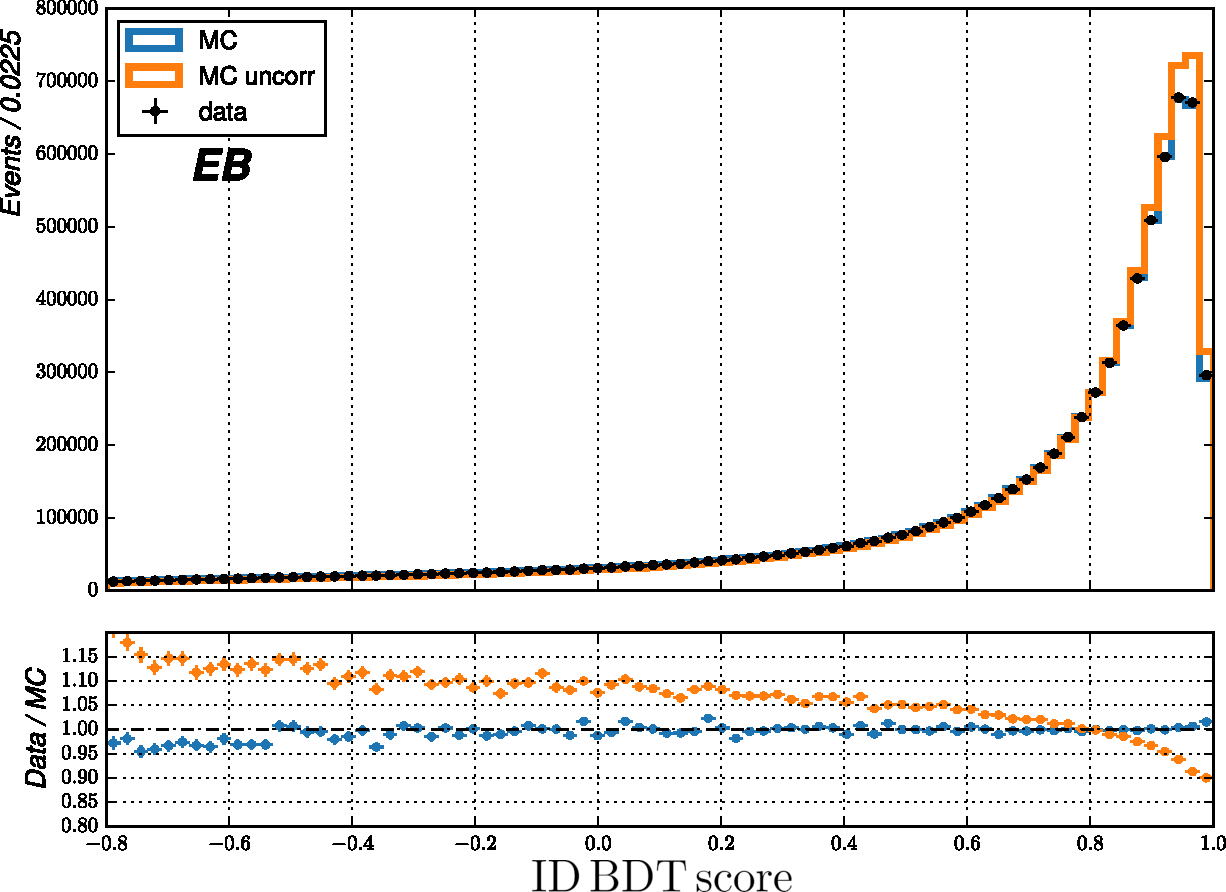
\includegraphics[width=.5\textwidth]{Figures/hgg_overview/dataMC_probePhoIdMVA_0_corr.pdf}
  \caption[Corrections from the chained quantile regression method in the ID BDT output score]
  {
    Photon-ID BDT score distributions for probe electrons in \Zee events, where the probe electrons are reconstructed in the ECAL barrel. The black points correspond to data taken in 2017. The corresponding simulation is shown without corrections in orange, and with the CQR corrections in blue. The bottom panel shows the ratio of data to simulation. The improved agreement from applying the CQR corrections is shown to propagate to the photon-ID BDT output score.
  }
  \label{fig:photon_id_2}
\end{figure}

Each photon in an event is required to have a photon-ID BDT score $>-0.9$. Events which do not satisfy this criteria have already been removed from the plots in Figure~\ref{fig:photon_id_1}, hence why the $\gamma$+jet and jet+jet distributions do not peak at -1. This selection criteria reduces the contribution from the $\gamma$+jet and jet+jet background processes by over 70\%, whilst maintaining at least 99\% of signal events. The cut is purposely chosen to be loose in order to maintain reasonable statistics in the background simulation for training the event categorisation discriminants. Akin to the pre-selection criteria, the efficiency of this requirement is derived in simulation and data using the tag-and-probe method on \Zee events, and the events in simulation are scaled to match the efficiency in data. In addition, the photon-ID BDT score is used in numerous ways in the event categorisation.

\subsection{Vertex selection}\label{sec:vertex_selection}
Equation \ref{eq:mgg} shows that the diphoton mass resolution depends not only on the per-photon-energy resolutions, but also on the determination of the diphoton opening angle, $\theta$. For this, it is necessary to know the precise location of the primary hard-scattering vertex from which the photons originate. If the location is correctly determined within 1~cm of the true vertex position, the diphoton mass resolution is dominated by the photon-energy resolution. For events with additional objects such as charged leptons and jets, it is relatively easy to assign the primary vertex, due to the presence of distinct charged-particle tracks. On the other hand, for \Hgg events with no additional objects (e.g. ggH 0J), it becomes a more difficult problem. In the \Hgg analysis, the diphoton vertex is assigned from a collection of candidate primary vertices using a dedicated BDT, which is trained using ggH \Hgg simulated events and takes as input features related to the tracks recoiling against the diphoton system:

\begin{itemize}
    \item $\sum_i |\vec{p}^{\,i}_T|^2$,
    \item $-\sum_i (\vec{p}^{\,i}_T\cdot \vec{p}_T^{\,\gamma\gamma}/|\vec{p}_T^{\,\gamma\gamma}|)$,
    \item $(|\sum_i \vec{p}^{\,i}_T| - p_T^{\,\gamma\gamma})/(|\sum_i \vec{p}^{\,i}_T| + p_T^{\,\gamma\gamma})$,
    \item the total number of photon conversions in the tracker,
    \item the pull ($|z_{\rm{vtx}}-z_{\rm{e}}|/\sigma_z$) between the longitudinal positions of the reconstructed vertex, $z_{\rm{vtx}}$, and the vertex estimated using tracks from photon conversions, $z_e$, where $\sigma_z$ is the uncertainty in $z_{\rm{e}}$.
\end{itemize}

\noindent
In these observable definitions, the sums run over all PF tracks associated with a given vertex, labelled by the index $i$. The quantity $\vec{p}_T^{\,\gamma\gamma}$ corresponds to the transverse momentum of the diphoton system, measured with respect to the same vertex. The final two BDT input variables in the list are only included for events which contain tracks originating from photon conversions. 

The performance of the vertex assignment BDT is evaluated using \Zmumu events. Here, the vertices are reconstructed after omitting the muon tracks, in order to imitate a diphoton-like system. The vertex is then said to be correctly assigned by the BDT if the location is within 1~cm of the true vertex position. Figure \ref{fig:vertex_selection_0} (left) shows the efficiency of the vertex assignment as a function of the dimuon $p_T$, for both simulation and data, demonstrating an agreement within 2\% across the whole $p_T$ range. Correction factors are applied to simulation to match the fraction of correctly assigned vertices observed in data, keeping the total number of events constant. For inclusive \Hgg events, the efficiency of correctly assigning the diphoton vertex to be within 1~cm of the true vertex is roughly 79\%. This value rises for events with additional objects such as jets and charged leptons.

\begin{figure}
  \centering
  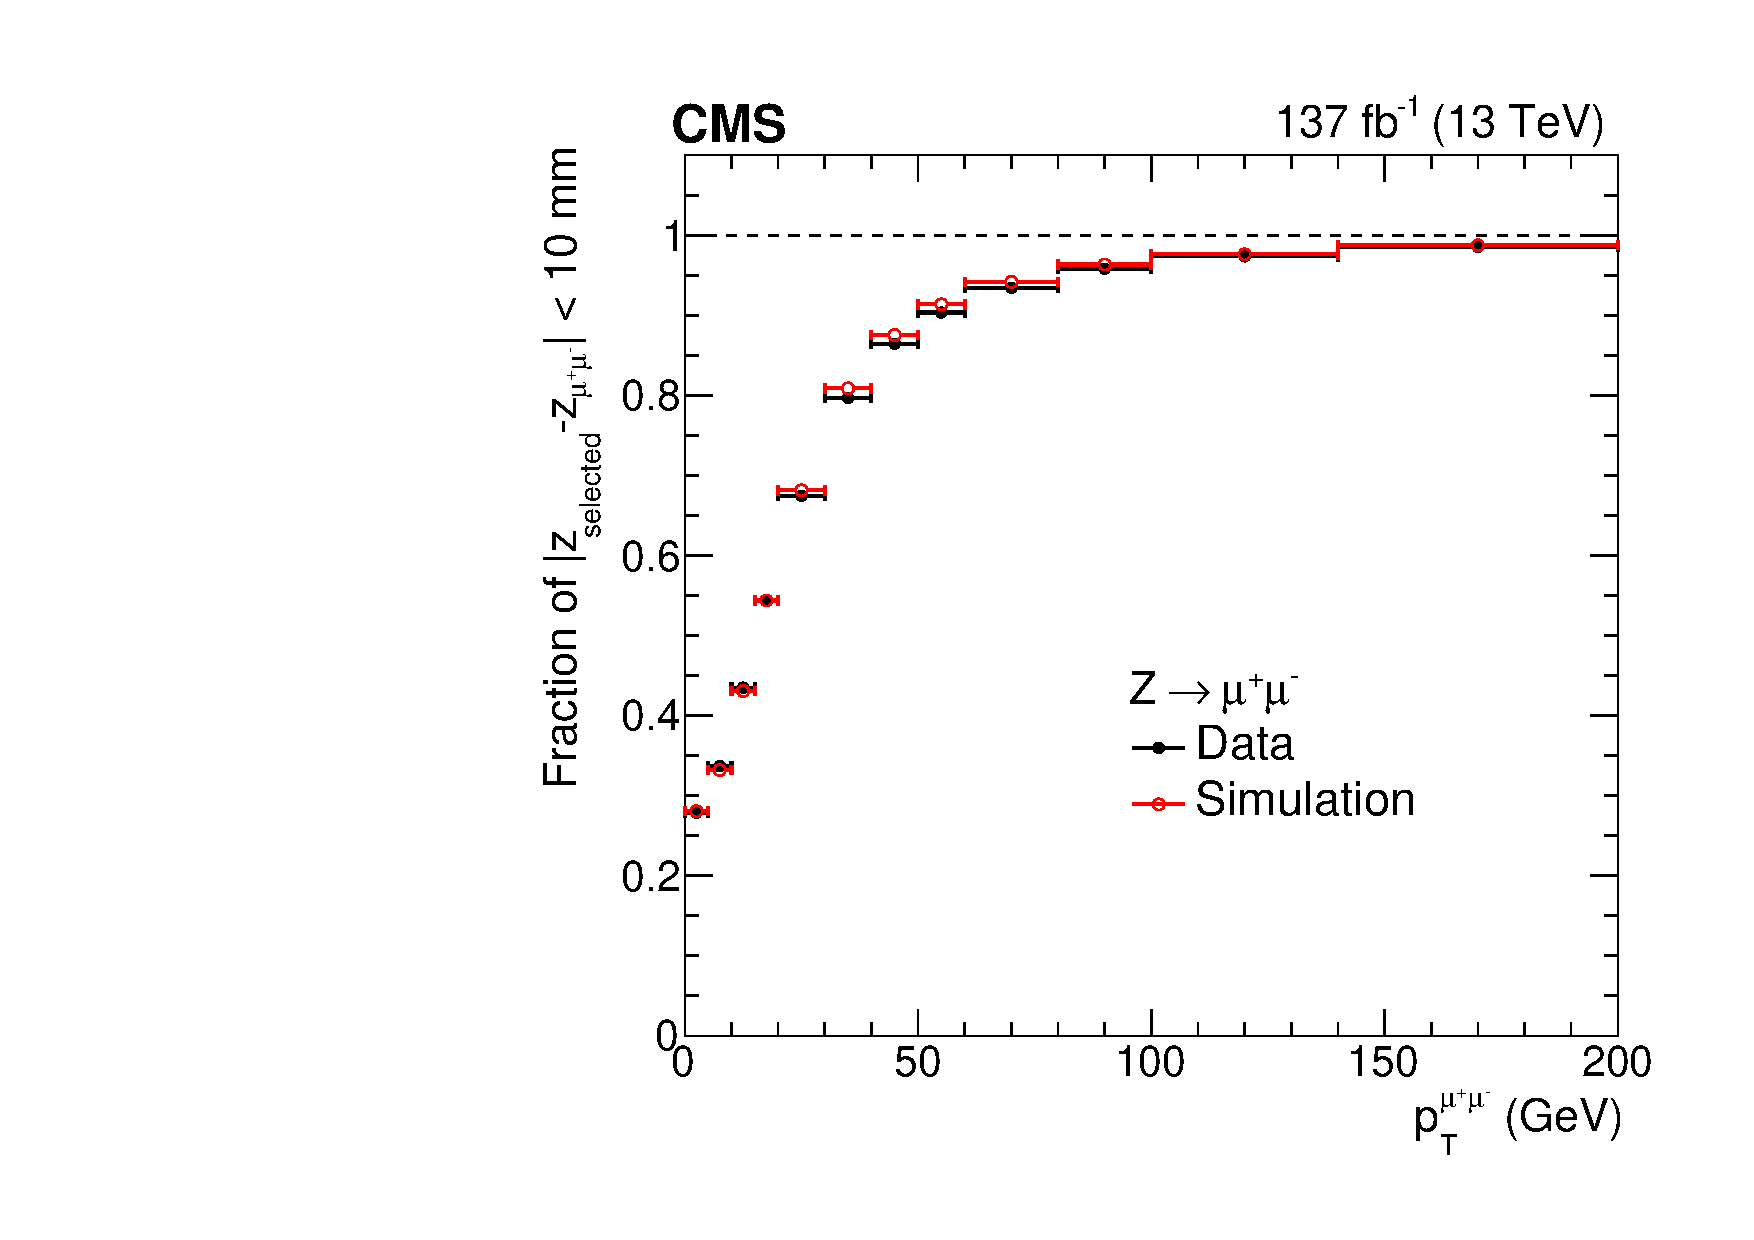
\includegraphics[width=.49\textwidth]{Figures/hgg_overview/Zmumu_eff_vs_pt_All.pdf}
  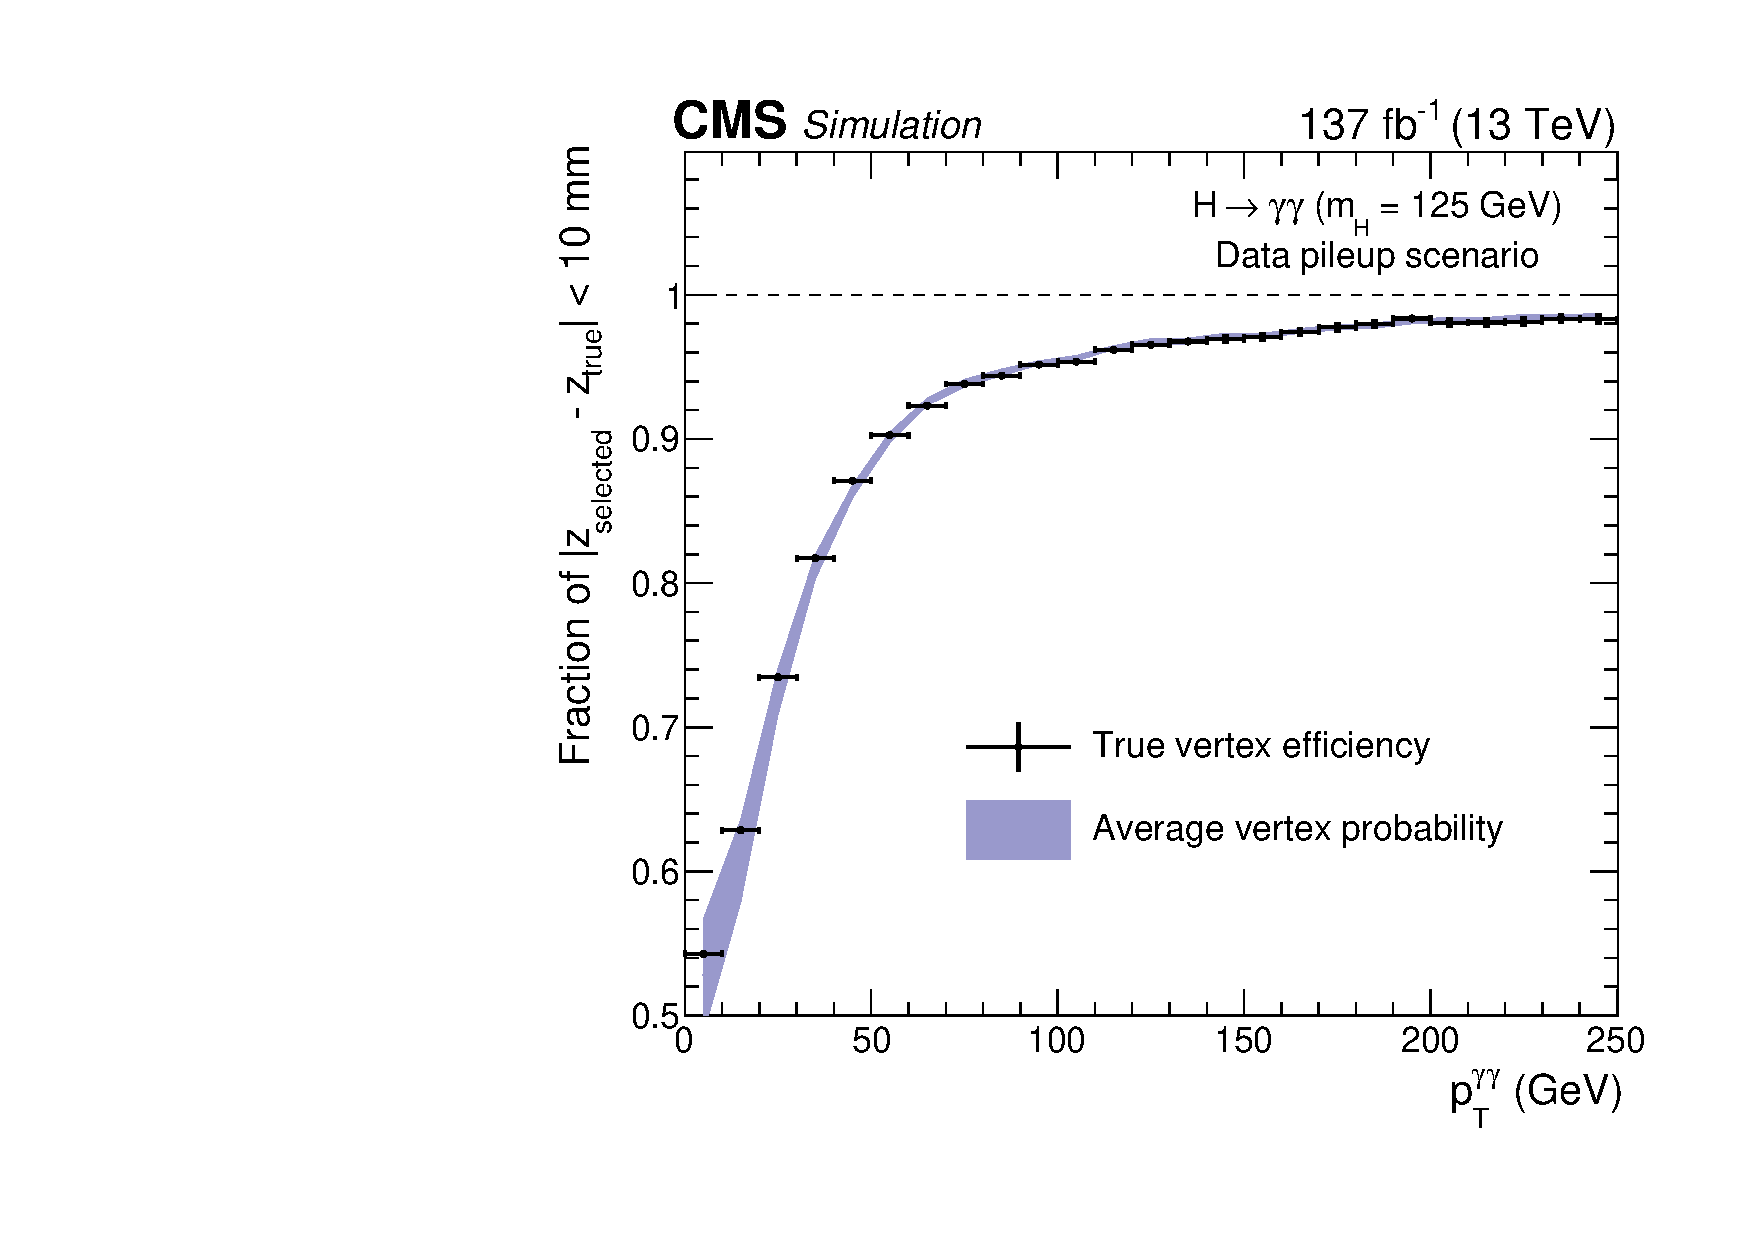
\includegraphics[width=.49\textwidth]{Figures/hgg_overview/AverageProbPlotFullRunIIVersusPt.pdf}
  \caption[Vertex-assignment and vertex-probability BDT]
  {
    The left plot shows the fraction of \Zmumu events where the assigned vertex is within 1~cm of the true vertex position as a function of $p_T^{\mu\mu}$, for simulated events in red and data events in black. Here, the muon tracks are omitted from the event reconstruction to mimic a \Hgg system. Simulated events are weighted to match the pileup and beamspot width distributions observed in data. The right plot demonstrates that the average vertex-probability BDT score agrees with the true vertex-assignment efficiency in simulated events. The full data set collected in the period 2016-2018 and the corresponding simulation are shown in the plots.
  }
  \label{fig:vertex_selection_0}
\end{figure}

An additional vertex-related BDT is trained to estimate the \textit{probability} that the vertex assignment is within 1~cm of the interaction point from which the diphoton originates. The input features are the total number of reconstructed vertices in an event, the relative positions and respective vertex assignment BDT scores for the three highest scoring vertices, $|{p}_T^{\,\gamma\gamma}|$, as well as the number of converted photons in the tracker. Akin to the vertex-assignment BDT, this vertex-probability BDT is trained using ggH, \Hgg events. The right-hand plot of Figure \ref{fig:vertex_selection_0} demonstrates the agreement between the output probability and the true vertex assignment efficiency in simulated events.

Finally, the width of the $z$ distribution of reconstructed vertices, known as the beamspot width, is measured to be between 3.4--3.6~cm in data. A year-dependent correction is applied to simulated events to ensure the beamspot width matches that observed in data.

\subsection{Reconstruction of other objects}\label{sec:hgg_otherobjects}
The analysis categories are defined to target events from different STXS bins. In order to define such categories it is necessary to place requirements on additional, reconstructed objects in the event, such as two forward-jets in VBF production or two-same flavour, oppositely-charged leptons in Z($\ell\ell$)H production. The following section briefly describes the reconstruction of these additional objects from the PF collections, described in Section~\ref{sec:particle_flow}.

\subsubsection{Jets}
The precise reconstruction of jets is particularly important in this analysis, not only for differentiating between different Higgs boson production modes, but also for splitting events according to the jet-related STXS boundaries: the number of jets, $m_{jj}$ and $p_T^{Hjj}$. On average, a jet carries 65\% of its total energy in charged hadrons, 25\% in photons, and the final 10\% in neutral hadrons. By providing separate collections of such final-state particles with independent measurements of their energies, the PF algorithm offers unprecedented performance in terms of the jet reconstruction at CMS. 

Jets are built by clustering the reconstructed PF candidates using the infrared and collinear-safe anti-$k_T$ algorithm~\cite{Cacciari:2008gp,Cacciari:2011ma}, with a distance parameter of 0.4. A Charged-Hadron Subtraction (CHS) technique is applied to remove charged hadrons that are associated with vertices other than the primary vertex (as chosen by the vertex-assignment BDT) from the clustering procedure. This helps to mitigate the contribution to the jet momentum from pileup. The algorithm operates by defining a distance measure between PF candidates that depends on their $p_T$ and angular parameters (see equation~\ref{eq:antikt_distance}), and iteratively clusters the four-momentum vectors with the shortest distance measure. Once the shortest distance measure is between the cluster and the LHC beam, the procedure terminates and the clustered objects are defined as a jet. This is repeated until all PF candidates have been clustered. The jet momentum is then calculated as the vectorial sum of all the PF candidate momenta in the jet. From simulation, this is found to be, on average, within 5 to 10\% of the truth-level jet momentum over the whole $p_T$ spectrum and detector acceptance.

After building the jets, a set of corrections are applied to correct the jet-energy scale and resolution in both data and simulation~\cite{Khachatryan:2016kdb}. Firstly, an offset correction is applied to account for any remaining contributions from pileup. This depends on the event energy-density, $\rho$, and the jet $p_T^j$, $\eta^j$ and angular spread, $\Delta R_j$. Following this, corrections are derived from simulation to (on average) match the reconstruction-level jet energy to the truth-level jet energy. These are calculated in bins of $p_T^j$ and $\eta^j$ to account for variations in the response across the detector. Any residual discrepancies in the jet-energy scale between data and simulation are rectified using in situ measurements of the momentum balance in dijet, $\gamma$+jet, Z+jet, and multijet events. The jet energy resolution after the corrections is typically 15--20\% at 30~GeV, 10\% at 100~GeV, and 5\% at 1~TeV, for jets in the central region of the detector~\cite{Khachatryan:2016kdb}.

Finally, a pileup-identification BDT is trained to reduce the number of pileup-induced jets entering the analysis~\cite{Sirunyan:2020foa}. Such jets typically contain PF candidates from multiple pileup collisions, and therefore tend to be more broad and diffuse than jets originating from the hard process. In addition, they usually contain tracks which are not associated with the primary vertex. To make use of these observations, the input features to the BDT are variables related to the jet shape, and additional track variables related to the interaction vertex. A $p_T$ and $\eta$-dependent threshold is then placed on the output score of this BDT to reject pileup jets. On top of this, to be considered in the event selection, jets are required to have $p_T^j>25$~GeV, fall within $|\eta^j|<4.7$, and have an angular separation with respect to both photons, $\Delta R_{j,\gamma}>0.4$.

\subsubsection{b tagging}
Jets originating from b quarks typically contain tracks associated with secondary vertices, which are displaced from the hard-scatter primary vertex by a few~mm to 1~cm. This is a result of the non-negligible lifetime of B hadrons (1.5~ps), which traverse a measurable distance in the detector before decaying. The identification of such jets (b tagging) is crucial for isolating ttH and tH production events, since the top quarks almost always decay to b quarks. A deep neural network (DNN, see Refs.~\cite{hastie01statisticallearning,10.5555/3086952,bishop:2006:PRML}) algorithm has been trained~\cite{Sirunyan:2017ezt}, which takes secondary vertices and PF candidates as input features, and outputs a probability that a given jet has originated from the decay of a B hadron. The per-jet output probabilities are used in the event categorisation, both for the pre-selection of ttH and tH events, and as input features to numerous ML classification algorithms.

\subsubsection{Charged leptons}
Tagging on additional charged leptons is crucial for isolating VH and top-associated Higgs boson production events, where at least one vector boson decays leptonically: $W\rightarrow\ell\nu$ and $Z\rightarrow\ell\ell$. Electrons and muons are taken from the PF electron and muon collections respectively, and additional isolation and identification requirements are placed on both~\cite{Khachatryan:2015hwa,Sirunyan:2018fpa}. To be considered in the event categorisation, electrons are required to have $p_T^e>10$~GeV and be within $|\eta^e|<2.4$, excluding the barrel-endcap transition region, whilst muons must have $p_T^\mu>5$~GeV and fall within $|\eta^\mu|<2.4$.

\subsubsection{Missing transverse momentum}
The missing transverse momentum vector, \metv, is calculated as the negative vector \pt sum of all PF candidates in an event, and its magnitude is denoted as \met~\cite{Sirunyan:2019kia}. The reconstruction of \metv accounts for the energy scale corrections applied to the reconstructed jets in the event. This is a useful quantity for selecting signal processes with additional neutrinos, such as WH (ZH) production where the vector boson decays into a neutrino and a lepton (two neutrinos).

%%%%%%%%%%%%%%%%%%%%%%%%%%%%%%%%%%%%%%%%%%%%%%%%%%%%%%%%%%%%%%%%%%%%%%%%%%%%%%%%%%%%%%%%%%%%%%%%%
\newpage
\section{Event categorisation}\label{sec:event_categorisation}

\subsection{Overview}
After the event reconstruction, a total of 80 event categories are constructed in which the \mgg spectrum is fitted simultaneously to measure Higgs boson production cross sections and couplings. Each category imposes a set of selection criteria related to the features of both the reconstructed diphoton system and the additional objects in the event. The criteria of a given category are defined to maximise the sensitivity to events from a particular STXS region\footnote{This can be a single bin or group of bins if the statistics are insufficient.}.

Before applying the dedicated per-category selection criteria, all events are required to have at least two pre-selected photon candidates, satisfying $p_T^{\gamma 1}>m_{\gamma\gamma}/3$ and ${p_T^{\gamma 2}>m_{\gamma\gamma}/4}$, with a diphoton invariant mass in the range $100<m_{\gamma\gamma}<180$~GeV. By scaling the transverse momentum by $m_{\gamma\gamma}$ in the selection criteria, distortions at the lower end of the mass spectrum are prevented. Furthermore, both photons are required to be in the geometrical acceptance of the ECAL: $|\eta|<2.5$, excluding the transition region $1.44<|\eta|<1.57$ between the barrel and endcaps. We then construct the analysis categories by following the procedure described below.

\begin{enumerate}
    \item \textit{Global categories} are defined to be enriched with events originating from the different Higgs boson production modes. Dedicated selection cuts are defined based on the different event topologies. For example, VBF-like events are isolated by requiring a pair of jets (dijet) with an invariant mass, $m_{jj}>350$~GeV. To further boost the ratio of signal-to-background events, ML classification algorithms are trained to isolate the targeted signal process from both SM background processes and the other Higgs boson production modes. At least one of these so-called \textit{background-rejection discriminants} are used in each global category. In this analysis, global categories are defined to target the tHq, ttH, VH, VBF and ggH production modes, in a variety of final states.
    
    \item The next step is to divide the per-production-mode global categories into \textit{analysis regions} to differentiate between the different kinematic regions (bins) of the STXS framework. For ggH production, excluding the kinematic region with high dijet mass (\mjj~$>350$~GeV), the division is performed using a dedicated ML classifier with output classes corresponding to the ggH STXS bins. For the other production modes, the global categories are split according to the reconstructed equivalents of the truth-level variables defining the STXS boundaries e.g. $p_T^{\gamma\gamma}$ for $p_T^H$. These divisions are performed as long as there exists some statistical sensitivity to the split STXS bins. 
    %If not, then the targeted group of STXS bins are merged together in the final cross section measurements (see section \ref{sec:results_STXS}). 
    
    \item An analysis region can be further sub-divided according to the signal-to-background purity. This is performed by placing boundaries on the relevant background-rejection discriminant(s). The position of these boundaries is optimised independently in each region to maximise the sensitivity to the targeted STXS bin (or bins). The usual metric for this optimisation is the approximate median significance (AMS),
    \begin{equation}
        \rm{AMS} = \sqrt{2\Big((S_{68}+B_{68})\ln(1+S_{68}/B_{68})-S_{68}\Big)},
    \end{equation}
    \noindent
    where $S_{68}$ is the number of signal events from the targeted STXS bin (or bins) and $B_{68}$ the number of background events, both calculated within a $\pm1\sigma_{\rm{eff}}$ window of $m_{\rm{H}}$. Here, $\sigma_{\rm{eff}}$ is defined as the shortest interval containing 68\% of the total number of targeted signal events. The background estimate, $B_{68}$, is determined by fitting an exponential function to background events, either directly to data sidebands or to the MC simulated background events. In the limit of small $S_{68}/B_{68}$, the AMS reduces to the familiar $S_{68}/\sqrt{S_{68}+B_{68}}$ formula.
    
    The final \textit{analysis categories} designed to target the \textit{truth-level} STXS bins are referred to as ``tags", which are defined in decreasing order of the expected signal-to-background ratio. For example, the tag with the highest $S_{68}/B_{68}$, targeting the ggH 0J low \ptH STXS bin, is denoted as ``0J low \ptgg Tag0". The total number of tags is realised by a stopping criterion, where the expected AMS gain by introducing an additional boundary is below a threshold e.g. 5\% improvement.
\end{enumerate}

The data and simulation from all three years are merged together in each category. This provides larger statistics for the training of the numerous multivariate discriminants, and the subsequent optimisation of the selection criteria. In addition, the larger yields allow to better constrain the shape parameters of the per-category background models (see Section \ref{sec:bkg_modeling}). The potential gain in splitting each category by year, and thus exploiting the year-dependent mass-resolution information in the final fit, was found to be negligible. 

It is possible for any given event to pass the selection criteria for multiple analysis categories. A priority sequence is defined to ensure the analysis categories are truly orthogonal: each event is assigned to at most one category, choosing the category with the highest priority. The sequence is defined to prioritise rarer Higgs boson production modes, by ordering according to the expected number of signal events. In other words, global categories targeting a Higgs boson production mode with a lower expected signal-yield (rarer process) are given a higher priority.

A summary of all analysis categories is provided in Table \ref{tab:categorisation_overview}, ordered according to decreasing priority in the category sequence. Example Feynman diagrams are shown for the targeted Higgs boson production modes. The background-rejection discriminants are listed, as well as the methods for splitting the global categories to target the kinematic regions of the STXS framework. Finally, the number of tags for each targeted STXS bin (or bins) are shown, defined by placing boundaries on the respective background-rejection discriminants. A graphical schema of the analysis event categorisation procedure is provided in Appendix~\ref{app:event_categorisation}.

The remainder of this chapter provides additional detail concerning the construction, optimisation, and validation of the event categorisation workflow, and shows the performance in terms of the purity of the final analysis categories. For reference, Table \ref{tab:categorisation_discriminants} provides a summary of all the ML classifiers used in the categorisation. The classifiers mainly use the BDT algorithm, barring the DNN which is trained to discriminate ttH production from tHq production. In the table, the training samples, training software, and final outputs are listed. The full set of input features for each classifier are listed in Appendix~\ref{app:event_categorisation}. When training the various classifiers, the samples are first weighted according to their respective SM cross sections, and are subject to the initial selection cuts of the relevant global category. Often, the weights of each output class (e.g. signal and background) are then equalised in the training to improve the classifier performance.

\begin{table}
    \caption[Categorisation overview]{A summary of the analysis event categorisation, ordered according to decreasing priority in the category sequence. For each global category, an example Feynman diagram of the targeted process is shown. In addition, the background-rejection discriminants and the methods used to split the global category to target different kinematic regions of the STXS framework are listed. The final column shows the number of tags defined to target each bin or group of bins.}
    \label{tab:categorisation_overview}
    % \vspace{.5cm}
    \centering
    \tiny
    \renewcommand{\arraystretch}{1.3}
    \setlength{\tabcolsep}{2pt}
    \hspace*{-3cm}
        \begin{tabular}{p{1.8cm}<{\centering}|m{3cm}<{\centering}|c|p{2.3cm}<{\centering}|c|c}
    Global category & Example diagram & Bkg rej. discriminant & Splitting method to target STXS bins & Targeted STXS bin(s) & \# of tags \\ \hline
    tHq leptonic & \vspace{.1cm}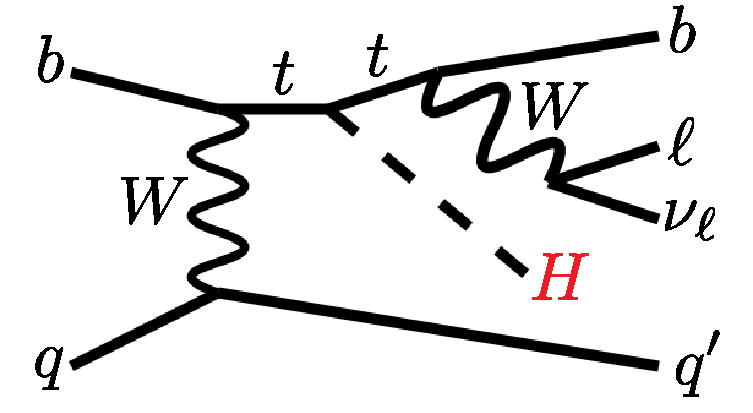
\includegraphics[width=3cm]{Figures/hgg_overview/categorisation_feynman/thq_lep.pdf} & \begin{tabular}{c}{tHq leptonic BDT-bkg\\top DNN (tH-vs-ttH)}\end{tabular} & None & tHq & 1 \\ \hline
    
    ttH leptonic & \vspace{.1cm}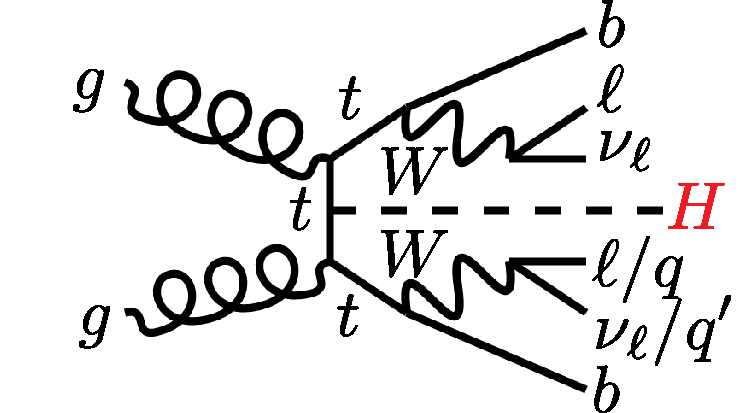
\includegraphics[width=3cm]{Figures/hgg_overview/categorisation_feynman/tth_lep.pdf} & \begin{tabular}{c}{ttH leptonic BDT-bkg\\top DNN (tH-vs-ttH)}\end{tabular} & Reco $p_T^{\gamma\gamma}$ & \begin{tabular}{c}{ttH~\ptH~$<$~60 \\ ttH~120~$<$~\ptH~$<$~120 \\ ttH~120~$<$~\ptH~$<$~200 \\ ttH~200~$<$~\ptH~$>$~300 \\ ttH~\ptH~$>$~300}\end{tabular} & \begin{tabular}{c}{2 \\ 2 \\ 2 \\ 1 \\ 1}\end{tabular} \\ \hline
    
    ZH leptonic & \vspace{.1cm}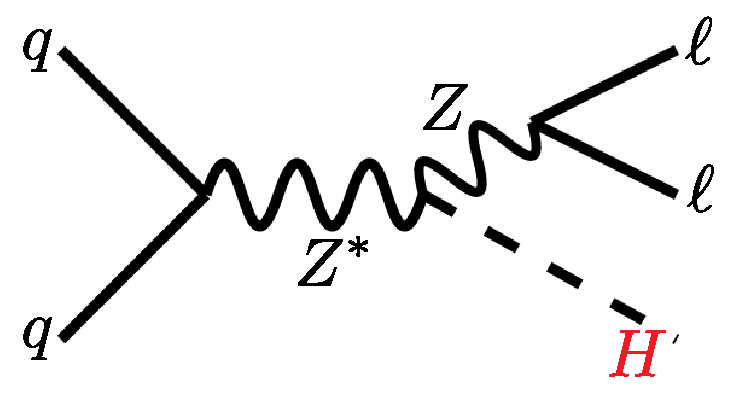
\includegraphics[width=3cm]{Figures/hgg_overview/categorisation_feynman/zh_lep.pdf} & ZH leptonic BDT & None & All ZH lep and ggZH lep bins (10) & 2 \\ \hline
    
    WH leptonic & \vspace{.1cm}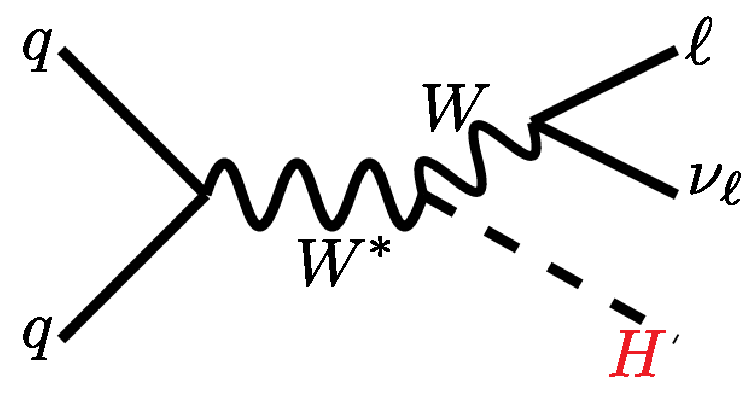
\includegraphics[width=3cm]{Figures/hgg_overview/categorisation_feynman/wh_lep.pdf} & WH leptonic BDT & Reco $p_T^{\gamma\gamma}$ & \begin{tabular}{c}{WH lep~$p_T^V<75$ \\ WH lep~$75<p_T^V<150$ \\ WH lep~$p_T^V>150$ (3)}\end{tabular} & \begin{tabular}{c}{2 \\ 2 \\ 1}\end{tabular} \\ \hline
    
    VH MET & \vspace{.1cm}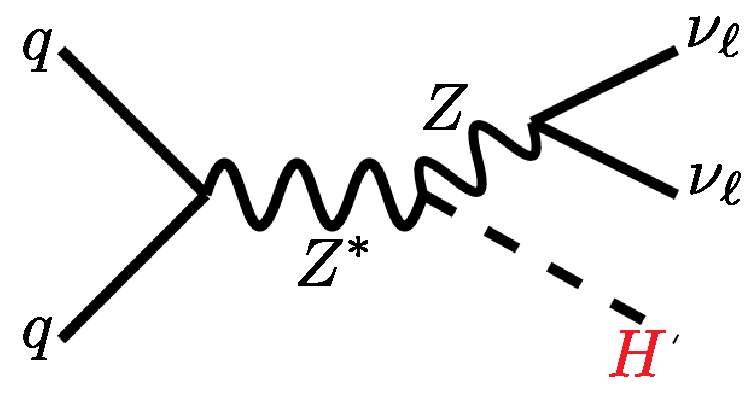
\includegraphics[width=3cm]{Figures/hgg_overview/categorisation_feynman/vh_met.pdf} & VH MET BDT & None & All VH lep bins (15) & 3 \\ \hline
    
    ttH hadronic & \vspace{.1cm}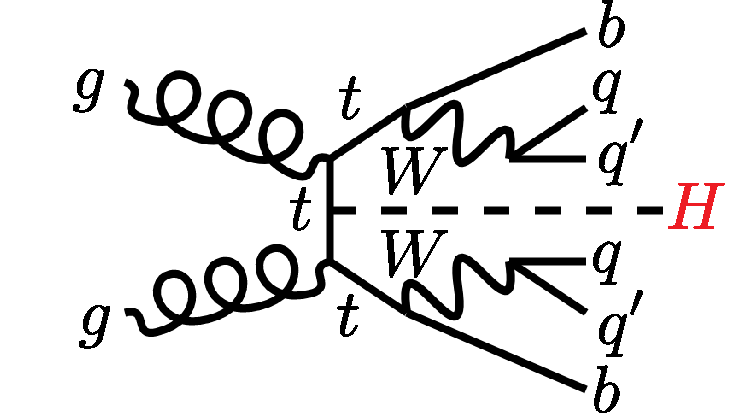
\includegraphics[width=3cm]{Figures/hgg_overview/categorisation_feynman/tth_had.pdf} & ttH hadronic BDT-bkg & Reco $p_T^{\gamma\gamma}$ & \begin{tabular}{c}{ttH~\ptH~$<$~60 \\ ttH~120~$<$~\ptH~$<$~120 \\ ttH~120~$<$~\ptH~$<$~200 \\ ttH~200~$<$~\ptH~$>$~300 \\ ttH~\ptH~$>$~300}\end{tabular} & \begin{tabular}{c}{2 \\ 2 \\ 2 \\ 2 \\ 2}\end{tabular} \\ \hline
    
    \multirow{2}{*}{VBF-like} & \vspace{.1cm}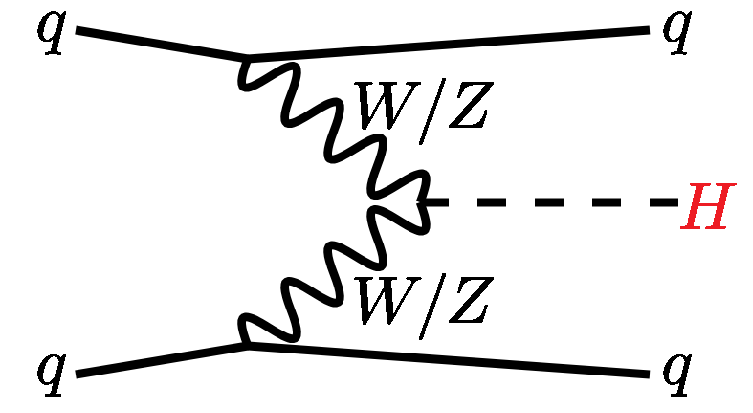
\includegraphics[width=3cm]{Figures/hgg_overview/categorisation_feynman/vbf.pdf} & \multirow{2}{*}{\begin{tabular}{c}{Dijet BDT\\Diphoton BDT}\end{tabular}} & Reco $p_T^{\gamma\gamma}$, $p_T^{\gamma\gamma jj}$, $m_{jj}$ & \begin{tabular}{c}{qqH BSM \\ qqH VBF-like low $m_{jj}$ low $p_T^{Hjj}$ \\ qqH VBF-like low $m_{jj}$ high $p_T^{Hjj}$ \\ qqH VBF-like high $m_{jj}$ low $p_T^{Hjj}$ \\ qqH VBF-like high $m_{jj}$ high $p_T^{Hjj}$ }\end{tabular} & \begin{tabular}{c}{2 \\ 2 \\ 2 \\ 2 \\ 2}\end{tabular} \\ \cline{2-2} \cline{4-6}
    & \vspace{.1cm}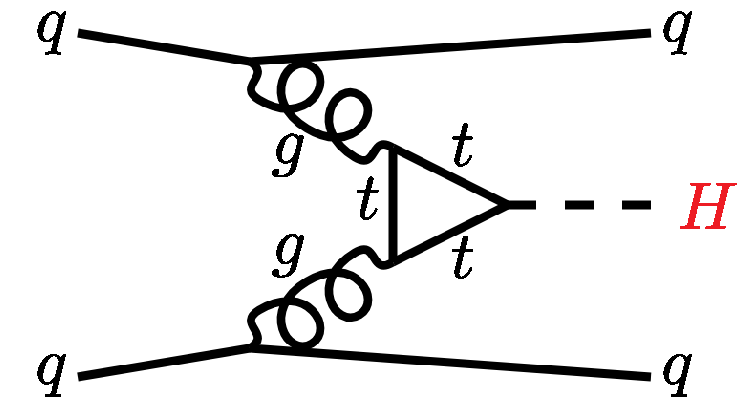
\includegraphics[width=3cm]{Figures/hgg_overview/categorisation_feynman/ggh_vbflike.pdf} & & None & All ggH VBF-like bins (4) & 2 \\ \hline
    
    VH hadronic & \vspace{.1cm}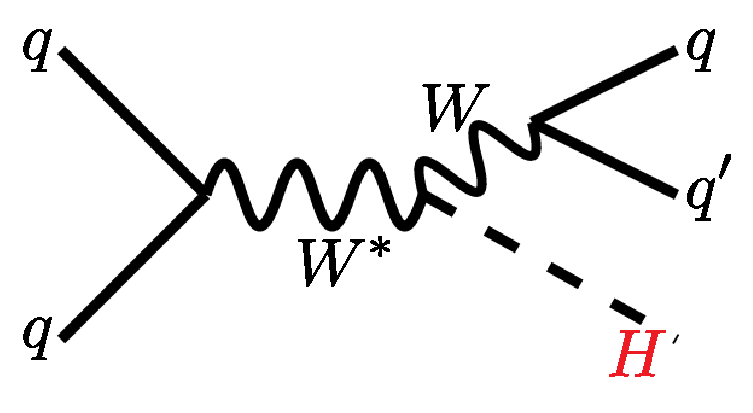
\includegraphics[width=3cm]{Figures/hgg_overview/categorisation_feynman/vh_had.pdf} & \begin{tabular}{c}{VH hadronic BDT\\Diphoton BDT}\end{tabular} & None & qqH VH-like & 2 \\ \hline
    
    ggH & \vspace{.1cm}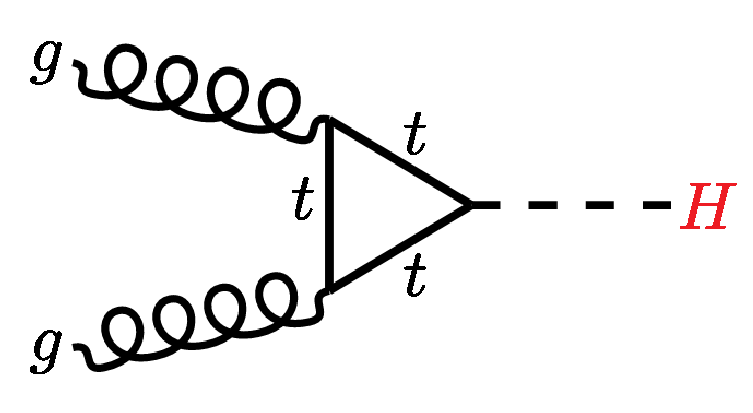
\includegraphics[width=3cm]{Figures/hgg_overview/categorisation_feynman/ggh.pdf} & Diphoton BDT & ggH BDT + Reco $p_T^{\gamma\gamma}$ for high \ptH region & \begin{tabular}{c}{ggH 0J low \ptH \\ ggH 0J high \ptH \\ ggH 1J low \ptH \\ ggH 1J med \ptH \\ ggH 1J high \ptH \\ ggH $\geq$2J low \ptH \\ ggH $\geq$2J med \ptH \\ ggH $\geq$2J high \ptH \\ ggH $200<p_T^H<300$ \\ ggH $300<p_T^H<450$ \\ ggH $450<p_T^H<650$ \\ ggH $p_T^H>650$}\end{tabular} & \begin{tabular}{c}{3 \\ 3 \\ 3 \\ 3 \\ 3 \\ 3 \\ 3 \\ 3 \\ 2 \\ 2 \\ 1 \\ 1}\end{tabular} \\ \hline
    
    No dedicated category & - & - & - & \begin{tabular}{c}{qqH 0J, 1J, $\geq$2J $m_{jj}<60$ \\ qqH $\geq$2J $120<m_{jj}<350$ \\ bbH, tHW}\end{tabular} & 0 \\ \hline
    
    \multicolumn{5}{r|}{Total$\quad$} & 73 \\
    \end{tabular}
    \hspace*{-3cm}
\end{table}

% \newgeometry{left=0.7in,right=0.5in,top=45mm,bottom=35mm}
% \begin{landscape}
% \thispagestyle{empty}
% % \hspace*{-5cm}
% \begin{table}
%     \caption[Categorisation multivariate classifiers]{A summary of the multivariate classifiers used in this analysis. Each classifier is trained using the listed samples after applying the initial selection criteria of the relevant global category. In the list of samples, top-associated backgrounds correspond to events containing at least one top quark and at least two reconstructed photons, such as tt+$\gamma\gamma$ or tt+$\gamma$+jet where the jet is misidentified as a photon.  The training software, input features, and the output of the various classifiers are listed. Usually, the weights of each output class are equalised in training to improve the performance of the classifiers. For the input features, photons, jets, b-tagged jets and leptons are labelled as $\gamma$, $j$, $bj$, and $\ell$, respectively, and the numbers represent the $p_T$-ordered list of the respective objects e.g. $\gamma 1$ corresponds to the leading photon. In the final two discriminants, $\rm{fwd}$ corresponds to the jet with the highest $|\eta|$. Definitions of the less obvious input features are provided in Appendix~\ref{app:event_categorisation}.}
%     \label{tab:categorisation_discriminants}
%     % \vspace{.5cm}
%     \centering
%     \tiny
%     \renewcommand{\arraystretch}{2.5}
%     \setlength{\tabcolsep}{3pt}
%     \hspace*{-2.5cm}
%     \begin{tabular}{l|c|m{6cm}<{\centering}|m{12cm}<{\centering}|m{4.5cm}<{\centering}}
    Discriminant/Classifier & Software & Training samples (simulation unless stated) & Input features, $\vec{x}$ & Output \\ \hline
    ggH BDT & \textsc{XGBoost} & ggH & $p_T^{\gamma 1/\gamma 2}/m_{\gamma\gamma}$, $\eta^{\gamma 1/\gamma 2}$, $\cos{\Delta\phi_{\gamma\gamma}}$, $\gamma 1/\gamma 2$ ID BDT scores, $\sigma_{RV}$, $\sigma_{WV}$, vertex probability BDT score, $p_T^{\gamma\gamma}$, $N_{\rm{jets}}$, $m_{jj}$, $\eta^{j1/j2/j3}$, $j1/j2/j3$ pile-up identification BDT scores, $\Delta\phi_{\gamma\gamma,j1/j2/j3}$, $\Delta\eta_{\gamma\gamma,j1/j2/j3}$ & 9 ggH STXS class probabilities: {\tiny 0J~low~\ptH, 0J~high~\ptH, 1J~low~\ptH, 1J~med~\ptH, 1J~high~\ptH, $\geq$2J~low~\ptH, $\geq$2J~med~\ptH, $\geq$2J~high~\ptH, $p_T^H>200$} \\ \hline
    
    Diphoton BDT & \textsc{XGBoost} & \makecell*{S: all Higgs boson events \\ B: SM $\gamma\gamma$} & $p_T^{\gamma 1/\gamma 2}/m_{\gamma\gamma}$, $\eta^{\gamma 1/\gamma 2}$, $\cos{\Delta\phi_{\gamma\gamma}}$, $\gamma 1/\gamma 2$ ID BDT scores, $\sigma_{RV}$, $\sigma_{WV}$, vertex probability BDT score & S-vs-B score \\ \hline
    
    Dijet BDT & \textsc{XGBoost} & VBF, ggH, SM $\gamma\gamma$ + data-driven estimate for $\gamma$+jet \& jet+jet & $p_T^{\gamma 1/\gamma 2}/m_{\gamma\gamma}$, $p_T^{\gamma\gamma}/m_{\gamma\gamma}$, $\cos{\Delta\phi_{\gamma\gamma}}$, $p_T^{j1/j2}$, $m_{jj}$, $\Delta\phi_{\gamma\gamma,jj}$, min($\Delta R_{\gamma,j}$), $C_{\gamma\gamma}$, $|\Delta\eta_{jj}|$, $\Delta\phi_{jj}$ & \makecell{3 output class probabilities: \\ {\tiny VBF, ggH, bkg}} \\ \hline
    
    VH hadronic BDT & \textsc{XGBoost} & \makecell*[{{m{6cm}}}]{\centering S: VH hadronic \\ B: ggH, SM $\gamma\gamma$ + data-driven estimate for $\gamma$+jet \& jet+jet} & $p_T^{\gamma 1/\gamma 2}/m_{\gamma\gamma}$, $p_T^{j1/j2}$, $\eta^{j1/j2}$, $m_{jj}$, $|\Delta\eta_{jj}|$, $\cos{\theta^*}$ & S-vs-B score \\ \hline    
    
    VH MET BDT & \textsc{TMVA} & \makecell*[{{m{6cm}}}]{\centering S: VH 0-leptons \\ B: other H prod modes, SM $\gamma\gamma$, Drell-Yan, diboson, top quark prod. + data-driven estimate for $\gamma$+jet} & $p_T^{\gamma 1/\gamma 2}/m_{\gamma\gamma}$, $\eta^{\gamma 1/\gamma 2}$, $\cos{\Delta\phi_{\gamma\gamma}}$, max/min $\gamma$ ID BDT scores, \met, $H_T$, $N_{\rm{jets}}$, $p_T^{j1}$, max jet b-tag score (deepCSV), $\Delta\phi_{\gamma\gamma,\met}$, min($\Delta\phi_{\met,j})$, $(p_T^{\gamma\gamma}-\met)/p_T^{\gamma\gamma}$ & S-vs-B score \\ \hline
    
    WH leptonic BDT &  \textsc{TMVA} & \makecell*[{{m{6cm}}}]{\centering S: VH 1-lepton \\ B: other H prod modes, SM $\gamma\gamma$, $\gamma$+jet, Drell-Yan, diboson, top-associated bkgs} & $p_T^{\gamma 1/\gamma 2}/m_{\gamma\gamma}$, $\eta^{\gamma 1/\gamma 2}$, $\cos{\Delta\phi_{\gamma\gamma}}$, max/min $\gamma$ ID BDT scores, $\gamma 1/\gamma 2$ pixel seed veto, $p_T^\ell$, $\eta^\ell$, $\Delta R_{\gamma 1/\gamma 2,\ell}$, $\Delta\theta_{\gamma\gamma,\ell}$, \met, $m_T$, $N_{\rm{jets}}$, $p_T^{j1}$, $j1/j2$ b-tag score (deepCSV) & S-vs-B score \\ \hline
    
    ZH leptonic BDT &  \textsc{TMVA} & \makecell*[{{m{6cm}}}]{\centering S: VH $\geq$2-leptons \\ B: other H prod modes, SM $\gamma\gamma$, $\gamma$+jet, Drell-Yan, diboson, top-associated bkgs} & $p_T^{\gamma 1/\gamma 2}/m_{\gamma\gamma}$, $\eta^{\gamma 1/\gamma 2}$, $\cos{\Delta\phi_{\gamma\gamma}}$, max/min $\gamma$ ID BDT scores, $\gamma 1/\gamma 2$ pixel seed veto, $p_T^{\ell 1/\ell 2}$, $\eta^{\ell 1/\ell 2}$, $\Delta R_{\gamma 1/\gamma 2,\ell 1/\ell 2}$, $\Delta\theta_{\gamma\gamma,\ell\ell}$, $m_{\ell\ell}$, $N_{\rm{jets}}$, $p_T^{j1}$, $j1$ b-tag score (deepCSV) & S-vs-B score \\ \hline

    ttH hadronic BDT-bkg &  \textsc{XGBoost} & \makecell*[{{m{6cm}}}]{\centering S: ttH 0-leptons, $\geq$3-jets ($\geq$1 b-tagged) \\ B: other H prod modes, SM $\gamma\gamma$, Drell-Yan, V+$\gamma$, diboson, top-associated bkgs + data-driven estimate for $\gamma$+jet \& jet+jet} & $p_T^{\gamma 1/\gamma 2}/m_{\gamma\gamma}$, $\eta^{\gamma 1/\gamma 2}$, max/min $\gamma$ ID BDT scores, $\gamma 1/\gamma 2$ pixel seed veto, $p_T^{\gamma\gamma}/{m_{\gamma\gamma}}$, $Y_{\gamma\gamma}$, $|\cos{\Delta\phi_{\gamma\gamma}}|$, $\Delta R_{\gamma\gamma}$, $\cos{\theta_H}$, $p_T^{j1/j2/j3/j4}$, $\eta^{j1/j2/j3/j4}$, $j1/j2/j3/j4$ b-tag score (DeepJet), max/min b-tag score, $N_{\rm{jets}}$, $H_T$, \met, DNN scores: ttH vs tt$\gamma\gamma$ (had) and ttH vs $\gamma\gamma$+jets (had), Top tagger BDT score & S-vs-B score \\ \hline
    
    ttH leptonic BDT-bkg &  \textsc{XGBoost} & \makecell*[{{m{6cm}}}]{\centering S: ttH $\geq$0-leptons, $\geq$1-jet \\ B: other H prod modes, SM $\gamma\gamma$, $\gamma$+jet, Drell-Yan, V+$\gamma$, diboson, top-associated bkgs} & $p_T^{\gamma 1/\gamma 2}/m_{\gamma\gamma}$, $\eta^{\gamma 1/\gamma 2}$, max/min $\gamma$ ID BDT scores, $\gamma 1/\gamma 2$ pixel seed veto, $p_T^{\gamma\gamma}/{m_{\gamma\gamma}}$, $Y_{\gamma\gamma}$, $|\cos{\Delta\phi_{\gamma\gamma}}|$, $\Delta R_{\gamma\gamma}$, $\cos{\theta_H}$, $p_T^{j1/j2/j3}$, $\eta^{j1/j2/j3}$, $j1/j2/j3$ b-tag score (DeepJet), max/min b-tag score, $N_{\rm{jets}}$, $H_T$, \met, $p_T^\ell$, $\eta^\ell$, $N_{\rm{leptons}}$ (tight ID), DNN scores: ttH vs tt$\gamma\gamma$ (lep) & S-vs-B score \\ \hline
    
    tHq leptonic BDT-bkg &  \textsc{TMVA} & \makecell*[{{m{6cm}}}]{\centering S: tHq leptonic \\ B: SM $\gamma\gamma$, $\gamma$+jet, top-associated bkgs} & $p_T^{\gamma 1/\gamma 2}/m_{\gamma\gamma}$, $\eta^{\gamma 1/\gamma 2}$, max/min $\gamma$ ID BDT scores, $\gamma 1/\gamma 2$ pixel seed veto, $N_{\rm{jets}}$, $N_{\rm{bjets}}$, $N_{\rm{jets}}$ with $|\eta|<1$, $p_T^{j1/j2/j3}$, $\eta^{j1/j2/j3}$, $p_T^{bj1/bj2/bj3}$, $\eta^{bj1/bj2/bj3}$, $p_T^{\rm{fwd}}$, $\eta^{\rm{fwd}}$, $\Delta\phi_{\gamma 1/\gamma 2,j1}$, $\Delta\phi_{\gamma 1/\gamma 2,\ell}$, $\Delta\phi_{\gamma 1/\gamma 2,bj1}$, $\Delta\phi_{\gamma 1/\gamma 2,{\rm{fwd}}}$, $p_T^\ell$, $\eta^\ell$ & S-vs-B score \\ \hline
    
    top DNN &  \makecell{\textsc{Keras}~+\\\textsc{TensorFlow}} & tHq and ttH & $p_T^{\gamma 1/\gamma 2}/m_{\gamma\gamma}$, $\eta^{\gamma 1/\gamma 2}$, max/min $\gamma$ ID BDT scores, $\gamma 1/\gamma 2$ pixel seed veto, $p_T^{\gamma\gamma}/{m_{\gamma\gamma}}$, $Y_{\gamma\gamma}$, $|\cos{\Delta\phi_{\gamma\gamma}}|$, $\Delta R_{\gamma\gamma}$, $\cos{\theta_H}$, $p_T^{j1/j2/j3}$, $\eta^{j1/j2/j3}$, $j1/j2/j3$ b-tag score (DeepJet), max/min b-tag score, $N_{\rm{jets}}$, $H_T$, \met, $p_T^\ell$, $\eta^\ell$, $N_{\rm{leptons}}$ (tight ID), $p_T^{\rm{fwd}}$, $\eta^{\rm{fwd}}$, $\ell 1/\ell 2$ charge & tHq-vs-ttH score \\
\end{tabular}
%     \hspace*{-2.5cm}
% \end{table}
% \end{landscape}
% \restoregeometry

% \hspace*{-5cm}
\begin{table}
    \caption[Categorisation ML classifiers]{A summary of the ML classifiers used in this analysis. Each classifier is trained using the listed samples after applying the initial selection criteria of the relevant global category. In the list of samples, top-associated backgrounds correspond to events containing at least one top quark and at least two reconstructed photons, such as tt+$\gamma\gamma$ or tt+$\gamma$+jet where the jet is misidentified as a photon.  The software used to train the classifiers, and their respective outputs are also listed. Usually, the weights of each output class are equalised in training to improve the performance of the classifiers. The full set of input features for each classifier are provided in Appendix~\ref{app:event_categorisation}.}
    \label{tab:categorisation_discriminants}
    % \vspace{.5cm}
    \centering
    \scriptsize
    \renewcommand{\arraystretch}{3.5}
    \setlength{\tabcolsep}{3pt}
    \hspace*{-0.5cm}
    \begin{tabular}{l|c|m{6cm}<{\centering}|m{4.5cm}<{\centering}}
    \hline
    Discriminant/Classifier & Software & Training samples (simulation unless stated) & Output \\ \hline
    ggH BDT & \textsc{XGBoost} & ggH & 9 ggH STXS class probabilities: 0J~low~\ptH, 0J~high~\ptH, 1J~low~\ptH, 1J~med~\ptH, 1J~high~\ptH, $\geq$2J~low~\ptH, $\geq$2J~med~\ptH, $\geq$2J~high~\ptH, $p_T^H>200$ \\ \hline
    
    Diphoton BDT & \textsc{XGBoost} & \makecell*{S: all Higgs boson events \\ B: SM $\gamma\gamma$} & S-vs-B score \\ \hline
    
    Dijet BDT & \textsc{XGBoost} & VBF, ggH, SM $\gamma\gamma$ + data-driven estimate for $\gamma$+jet \& jet+jet & \makecell{3 output class probabilities: \\ {\tiny VBF, ggH, bkg}} \\ \hline
    
    VH hadronic BDT & \textsc{XGBoost} & \makecell*[{{m{6cm}}}]{\centering S: VH hadronic \\ B: ggH, SM $\gamma\gamma$ + data-driven estimate for $\gamma$+jet \& jet+jet} & S-vs-B score \\ \hline    
    
    VH MET BDT & \textsc{TMVA} & \makecell*[{{m{6cm}}}]{\centering S: VH 0-leptons \\ B: other H prod modes, SM $\gamma\gamma$, Drell-Yan, diboson, top quark prod. + data-driven estimate for $\gamma$+jet} & S-vs-B score \\ \hline
    
    WH leptonic BDT &  \textsc{TMVA} & \makecell*[{{m{6cm}}}]{\centering S: VH 1-lepton \\ B: other H prod modes, SM $\gamma\gamma$, $\gamma$+jet, Drell-Yan, diboson, top-associated bkgs} & S-vs-B score \\ \hline
    
    ZH leptonic BDT &  \textsc{TMVA} & \makecell*[{{m{6cm}}}]{\centering S: VH $\geq$2-leptons \\ B: other H prod modes, SM $\gamma\gamma$, $\gamma$+jet, Drell-Yan, diboson, top-associated bkgs} & S-vs-B score \\ \hline

    ttH hadronic BDT &  \textsc{XGBoost} & \makecell*[{{m{6cm}}}]{\centering S: ttH 0-leptons, $\geq$3-jets ($\geq$1 b-tagged) \\ B: other H prod modes, SM $\gamma\gamma$, Drell-Yan, V+$\gamma$, diboson, top-associated bkgs + data-driven estimate for $\gamma$+jet \& jet+jet} & S-vs-B score \\ \hline
    
    ttH leptonic BDT &  \textsc{XGBoost} & \makecell*[{{m{6cm}}}]{\centering S: ttH $\geq$0-leptons, $\geq$1-jet \\ B: other H prod modes, SM $\gamma\gamma$, $\gamma$+jet, Drell-Yan, V+$\gamma$, diboson, top-associated bkgs} & S-vs-B score \\ \hline
    
    tHq leptonic BDT &  \textsc{TMVA} & \makecell*[{{m{6cm}}}]{\centering S: tHq leptonic \\ B: SM $\gamma\gamma$, $\gamma$+jet, top-associated bkgs} & S-vs-B score \\ \hline
    
    Top DNN &  \makecell{\textsc{Keras}~+\\\textsc{TensorFlow}} & tHq and ttH & tHq-vs-ttH score \\
    \hline
\end{tabular}
    \hspace*{-0.5cm}
\end{table}

% \FloatBarrier
\newpage
\subsection{ggH categorisation}\label{sec:ggh_categorisation}

\begin{figure}
  \centering
  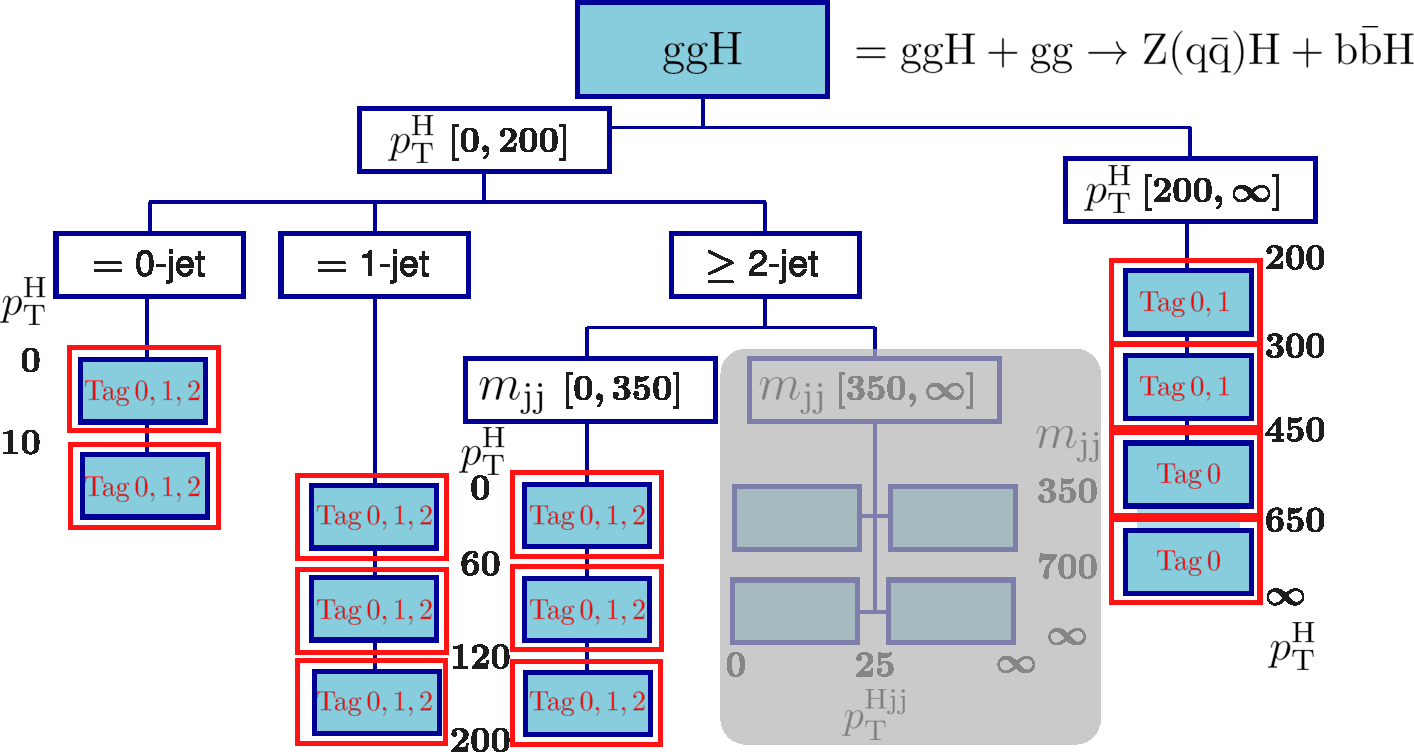
\includegraphics[width=.8\textwidth]{Figures/hgg_overview/categorisation_schematics/ggHSchematic.pdf}
  \caption[ggH categorisation schematic]
  {
    A schematic of the ggH categorisation scheme. The analysis categories, defined by the red boxes, surround their targeted STXS bin. The number of tags for each analysis region are highlighted in the plot. A shaded-grey region is shown for the STXS bins with a dijet invariant mass, $m_{jj}>350$~GeV, as they are not targeted in the ggH categorisation scheme.
  }
  \label{fig:ggH_categorisation_schematic}
\end{figure}

The final global category in the sequence targets the ggH production mode and considers all events that pass the photon pre-selection but are not selected by higher-priority categories. Firstly, the ggH BDT is used to predict the most probable ggH STXS region from which the event originates. The BDT outputs nine class-probabilities corresponding to the region with $p_T^H>200$~GeV and the two 0-jet, three 1-jet and three $\geq$2-jet STXS bins with $p_T^H<200$~GeV and $m_{jj}<350$~GeV. To minimise the dependence on the modelling of events with high $p_T^H$, the BDT is not trained to distinguish between the four bins with $p_T^H>200$~GeV; instead events in this class are further split into the final STXS bins using the reconstructed \ptgg. Events with a reconstructed dijet invariant mass $m_{jj}>350$~GeV are not assigned by the ggH BDT and are instead classified using the dijet BDT, as described in Section \ref{sec:qqH_categorisation}.

The nine ggH classes are uniquely defined by the Higgs boson transverse-momentum and the number of jets. It was found that the ggH BDT outperforms the assignment from using the reconstructed \ptgg and number of jets alone. This improvement arises as the BDT can exploit the correlations between the photon and jet kinematic properties, and thus use the well-measured photon quantities to infer information related to the less well-measured jets. As a result, the correct assignment of the per-event number of jets increases from 77\% to 82\%; the improvement is negligible for the \ptgg assignment since this is already a well-measured quantity with little migration across the \ptH boundaries. Propagating this to the final results leads to an improvement in the measured cross sections, particularly for the 0J and 1J bins ($\sim 10\%$ reduction in the uncertainty), and reduces the correlations between measured quantities.

The nine output class-probabilities are calculated for each event, and the event is subsequently assigned to the STXS region with the highest probability. The final 12 analysis regions (9 output ggH BDT classes, where the $p_T^H>200$~GeV class is further split using boundaries in the reconstructed \ptgg at 300, 450 and 650~GeV) are then divided into the final tags using the diphoton BDT. This BDT is trained to discriminate all Higgs boson signal from all other modes of SM diphoton production, meaning the output score, as shown in Figure \ref{fig:diphoton_score}, can be used to reduce the background contamination in each of the analysis regions. The boundaries on the diphoton BDT output are optimised independently in each region to maximise the expected AMS. Three tags are defined for each of the eight STXS bins with $p_T^H<200$~GeV, two for the two bins with ${200<p_T^H<450}$~GeV, and one for the two bins with $p_T^H>450$~GeV. The final set of analysis categories, with their respective targeted STXS bins, are shown by the red boxes in Figure~\ref{fig:ggH_categorisation_schematic}. Events that fail the lowest diphoton BDT output threshold in the respective region are discarded from the analysis. 

Clearly, the agreement between data and the background simulation is reasonably poor in certain bins of the diphoton BDT output distribution. This mis-modelling is likely to be improved in the future when samples generated at a higher order in perturbation theory are used for estimating the $\gamma$+jet and jet+jet contributions to the background. Nevertheless, the poor agreement does not manifest as a systematic uncertainty in the analysis, as the background model is estimated directly from data. Instead, it leads only to a sub-optimal performance of the diphoton BDT. This is a common trait for all ML classifiers used in the event categorisation, and is highlighted again when discussing the validation of the event categorisation in Section~\ref{sec:cat_validation}.

Table \ref{tab:ggH_category_yields} presents the expected signal and background yields in each of the ggH analysis categories. The signal yields are broken down into the fractional contribution from the target STXS bin, as well as the fractional contributions from the different Higgs boson production modes.

\begin{table}
    \caption[Expected yields for the ggH production mode categories]{The expected number of events for $m_{\rm{H}}=125$~GeV in the analysis categories targeting the ggH production mode, shown for an integrated luminosity of 137~\fbinv. The fraction of the total number of events arising from each production mode in each analysis category is provided, as is the fraction of events originating from the targeted STXS bin (or bins). Here, ggH includes contributions from the sub-dominant ggZ(q$\bar{\rm{q}}$)H production mode, qqH includes both VBF and V(q$\bar{\rm{q}}$)H production, and ``Top" represents both ttH and tH production together. The $\sigma_{\rm{eff}}$, defined as the smallest interval containing 68.3\% of the $m_{\gamma\gamma}$ distribution provides an indication of the mass resolution in each category. Also provided are the estimated number of background events-per-GeV in the signal peak region, the quantity $F_{68}=S_{68}/(S_{68}+B_{68})$, where $S_{68}$ and $B_{68}$ are the expected number of signal and background events in a $\pm1\sigma_{\rm{eff}}$ window centred on $m_{\rm{H}}$, respectively, and the approximate significance, $Z_{68}=S_{68}/\sqrt{S_{68}+B_{68}}$. The final column shows the significance for the targeted STXS bin (or bins) only, $Z^{\rm{target}}_{68}$,  where other Higgs boson signal events are considered as background.}
    \label{tab:ggH_category_yields}
    % \vspace{.5cm}
    \centering
    \scriptsize
    \renewcommand{\arraystretch}{1.3}
    \setlength{\tabcolsep}{3pt}
    \hspace*{-5cm}
    \begin{tabular}{l|ccccccccc}
    \multirow{3}{*}{Analysis categories} & \multicolumn{8}{c}{SM 125 GeV Higgs boson expected signal} & \multirow{3}{*}{S/S+B} \\ 
     & \multirow{2}{*}{\begin{tabular}[c]{@{}c@{}}Total\\Yield\end{tabular}} & \multirow{2}{*}{\begin{tabular}[c]{@{}c@{}}Target\\Fraction\end{tabular}} & \multicolumn{5}{c}{Production Mode Fractions} & \multirow{2}{*}{\begin{tabular}[c]{@{}c@{}}$\sigma_{\rm{eff}}$\\(GeV)\end{tabular}} & \\ 
     & & & ggH & bbH & qqH & VH lep & Top & & \\ \hline 
     0J low $\ptgg$ Tag0 & 294.2 & 86.5\% & 98.6\% & 1.1\% & 0.3\% & - & - & 1.93 & 0.06 \\ 
     0J low $\ptgg$ Tag1 & 340.0 & 89.6\% & 98.9\% & 1.0\% & 0.1\% & - & - & 2.29 & 0.03 \\ 
     0J low $\ptgg$ Tag2 & 292.7 & 89.7\% & 98.9\% & 1.0\% & 0.1\% & - & - & 2.51 & 0.01 \\ 
     [\cmsTabSkip]
     0J high $\ptgg$ Tag0 & 892.5 & 83.0\% & 97.0\% & 1.3\% & 1.6\% & - & - & 1.82 & 0.07 \\ 
     0J high $\ptgg$ Tag1 & 1156.7 & 79.8\% & 96.8\% & 1.4\% & 1.8\% & 0.1\% & - & 2.38 & 0.03 \\ 
     0J high $\ptgg$ Tag2 & 743.7 & 80.1\% & 96.9\% & 1.4\% & 1.6\% & 0.1\% & - & 2.62 & 0.01 \\ 
     [\cmsTabSkip]
     1J low $\ptgg$ Tag0 & 192.0 & 66.2\% & 89.9\% & 0.9\% & 8.7\% & 0.6\% & - & 1.62 & 0.09 \\ 
     1J low $\ptgg$ Tag1 & 283.5 & 66.3\% & 89.7\% & 0.8\% & 8.9\% & 0.6\% & - & 1.96 & 0.05 \\ 
     1J low $\ptgg$ Tag2 & 240.8 & 65.9\% & 89.8\% & 0.8\% & 8.8\% & 0.7\% & - & 2.35 & 0.02 \\ 
     [\cmsTabSkip]
     1J med $\ptgg$ Tag0 & 74.4 & 65.9\% & 81.5\% & 0.3\% & 17.6\% & 0.6\% & - & 1.62 & 0.18 \\ 
     1J med $\ptgg$ Tag1 & 215.1 & 68.8\% & 85.1\% & 0.5\% & 13.4\% & 1.0\% & - & 1.82 & 0.10 \\ 
     1J med $\ptgg$ Tag2 & 373.3 & 67.9\% & 85.0\% & 0.5\% & 13.4\% & 1.2\% & - & 2.04 & 0.05 \\ 
     [\cmsTabSkip]
     1J high $\ptgg$ Tag0 & 18.2 & 61.2\% & 77.6\% & 0.1\% & 22.2\% & 0.1\% & - & 1.46 & 0.35 \\ 
     1J high $\ptgg$ Tag1 & 60.4 & 63.2\% & 77.6\% & 0.1\% & 22.1\% & 0.1\% & - & 1.78 & 0.16 \\ 
     1J high $\ptgg$ Tag2 & 66.3 & 63.2\% & 78.1\% & 0.1\% & 21.2\% & 0.6\% & - & 2.02 & 0.06 \\ 
     [\cmsTabSkip]
     $\geq$2J low $\ptgg$ Tag0 & 18.4 & 53.1\% & 77.5\% & 0.6\% & 18.9\% & 0.8\% & 2.2\% & 1.47 & 0.06 \\ 
     $\geq$2J low $\ptgg$ Tag1 & 67.1 & 53.2\% & 76.3\% & 0.7\% & 19.6\% & 0.7\% & 2.7\% & 1.91 & 0.03 \\ 
     $\geq$2J low $\ptgg$ Tag2 & 39.0 & 49.0\% & 72.2\% & 0.6\% & 21.3\% & 0.8\% & 5.0\% & 2.31 & 0.01 \\ 
     [\cmsTabSkip]
     $\geq$2J med $\ptgg$ Tag0 & 25.4 & 63.5\% & 81.0\% & 0.1\% & 17.4\% & 0.1\% & 1.4\% & 1.49 & 0.16 \\ 
     $\geq$2J med $\ptgg$ Tag1 & 76.3 & 60.9\% & 79.3\% & 0.1\% & 18.5\% & 0.2\% & 1.9\% & 1.78 & 0.07 \\ 
     $\geq$2J med $\ptgg$ Tag2 & 122.3 & 59.5\% & 77.9\% & 0.1\% & 18.8\% & 0.5\% & 2.7\% & 2.09 & 0.03 \\ 
     [\cmsTabSkip]
     $\geq$2J high $\ptgg$ Tag0 & 37.6 & 67.3\% & 79.8\% & - & 18.5\% & 0.2\% & 1.6\% & 1.58 & 0.20 \\ 
     $\geq$2J high $\ptgg$ Tag1 & 25.9 & 67.0\% & 78.3\% & - & 19.6\% & 0.3\% & 1.8\% & 1.76 & 0.12 \\ 
     $\geq$2J high $\ptgg$ Tag2 & 70.1 & 61.3\% & 76.0\% & - & 20.6\% & 0.7\% & 2.8\% & 1.93 & 0.05 \\ 
     [\cmsTabSkip]
     BSM low $\ptgg$ Tag0 & 30.2 & 77.3\% & 79.1\% & - & 19.4\% & - & 1.5\% & 1.48 & 0.36 \\ 
     BSM low $\ptgg$ Tag1 & 36.5 & 72.6\% & 76.1\% & - & 21.2\% & - & 2.7\% & 1.89 & 0.11 \\ 
     [\cmsTabSkip]
     BSM med-low $\ptgg$ Tag0 & 14.8 & 77.3\% & 78.8\% & - & 18.9\% & 0.3\% & 2.0\% & 1.44 & 0.38 \\ 
     BSM med-low $\ptgg$ Tag1 & 4.5 & 66.7\% & 69.2\% & - & 22.5\% & 1.2\% & 7.1\% & 1.58 & 0.08 \\ 
     [\cmsTabSkip]
     BSM med-high $\ptgg$ & 3.0 & 58.3\% & 62.0\% & - & 31.4\% & 1.1\% & 5.6\% & 1.41 & 0.24 \\ 
     [\cmsTabSkip]
     BSM high $\ptgg$ & 0.8 & 73.0\% & 73.3\% & - & 21.2\% & 1.7\% & 3.7\% & 1.22 & 0.37 \\ 
     [\cmsTabSkip]
\end{tabular}

    \hspace*{-5cm}
\end{table}

\begin{figure}
  \centering
  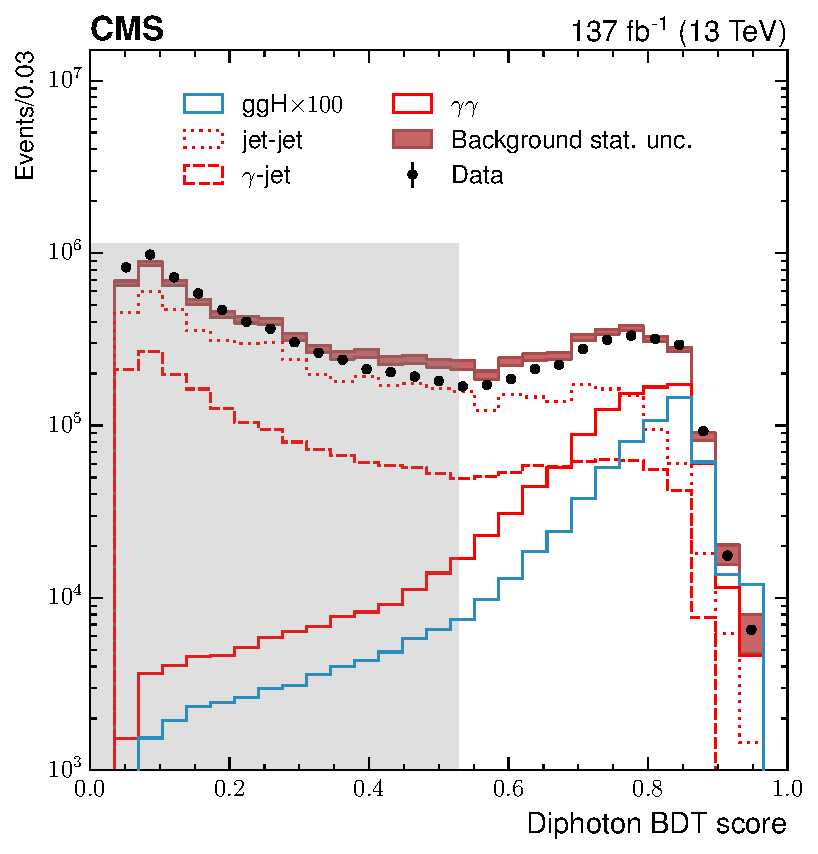
\includegraphics[width=.5\textwidth]{Figures/hgg_overview/DiphoBDT_dipho_mva_logPlot_noStack.pdf}
  \caption[Diphoton BDT output score]
  {
    The diphoton BDT score distribution for all events passing pre-selection and satisfying $100<m_{\gamma\gamma}<180$~GeV. Events from simulation and data are shown by the red band and the black points respectively. Histograms are shown for the different contributions of the simulated background in red. The blue histogram corresponds to simulated Higgs boson signal events, produced via ggH, multiplied by a factor of 100 to ease the comparison with the background distributions. The shaded grey region represents scores below the lowest diphoton BDT threshold used to define the final analysis tags. The full data set collected in the period 2016-2018 and the corresponding simulation is shown.
  }
  \label{fig:diphoton_score}
\end{figure}

\subsection{EW qqH categorisation}\label{sec:qqH_categorisation}
\begin{figure}
  \centering
  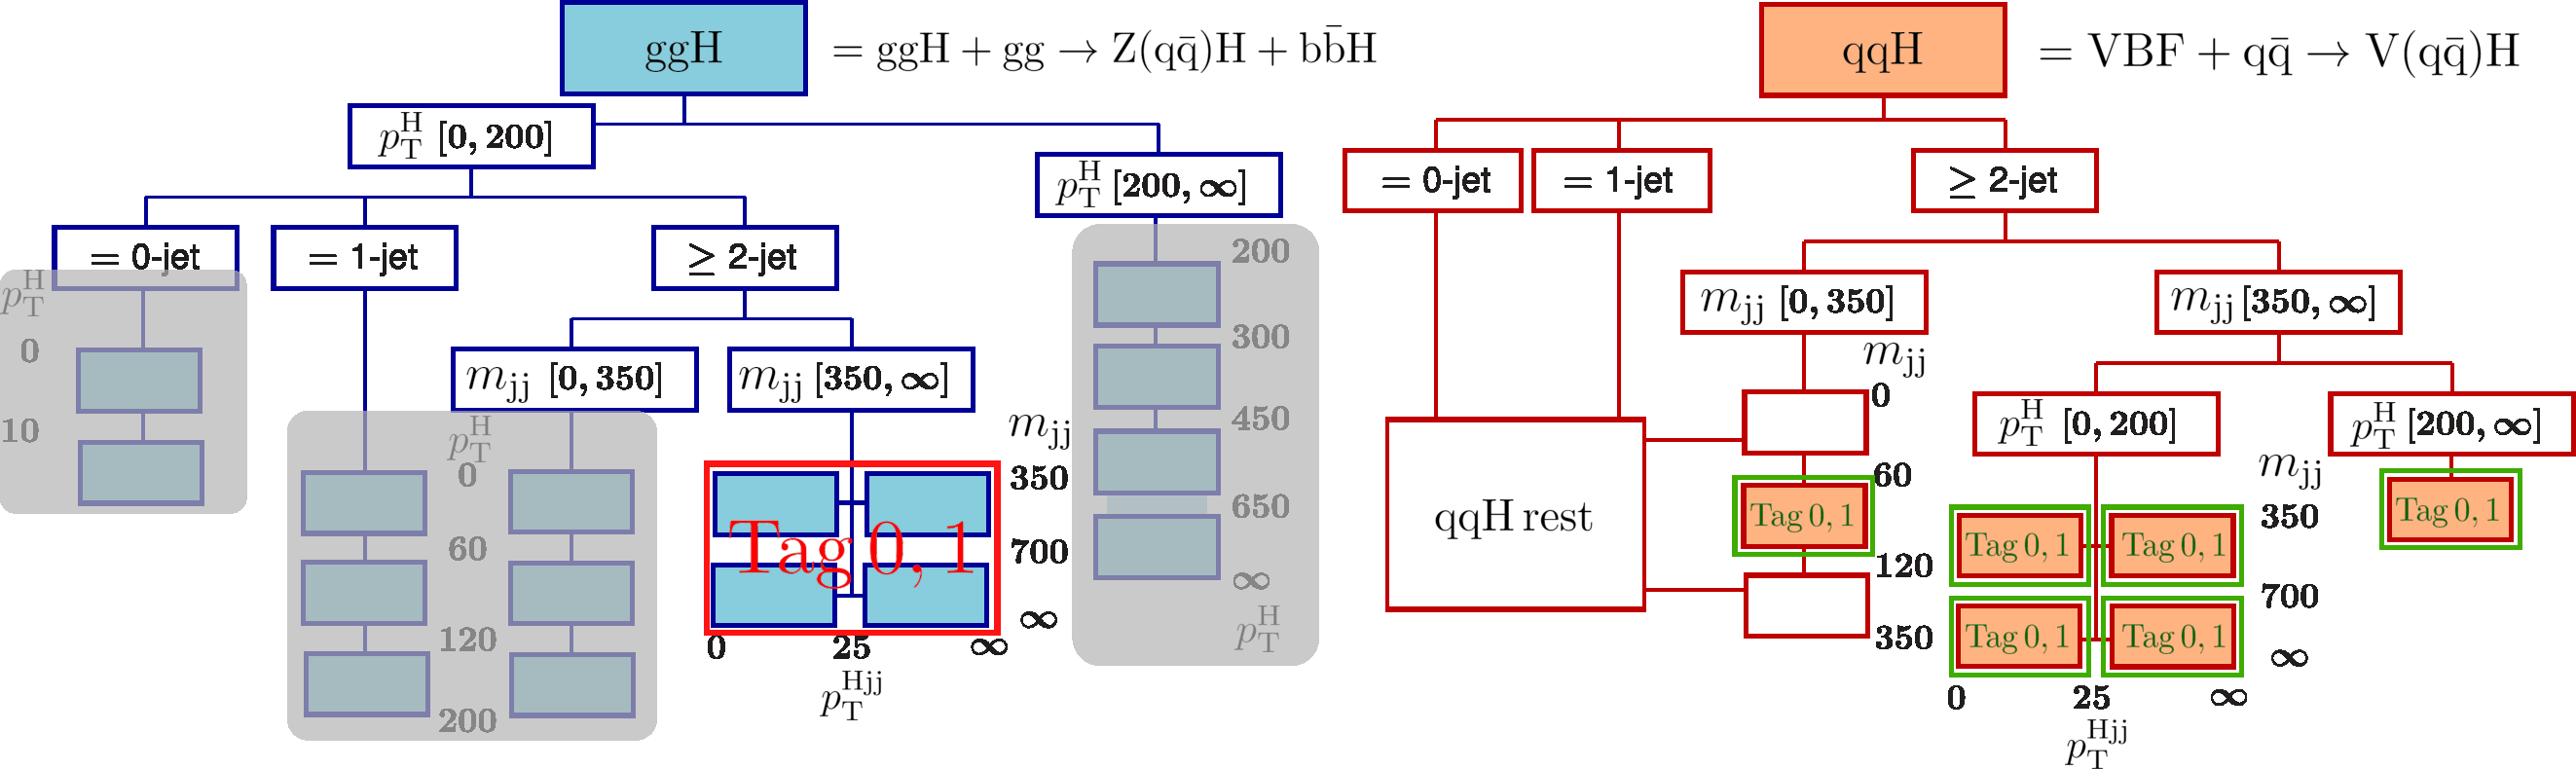
\includegraphics[width=1\textwidth]{Figures/hgg_overview/categorisation_schematics/qqHCategorisation.pdf}
  \caption[qqH and ggH VBF-like categorisation schematic]
  {
    A schematic of the qqH and ggH VBF-like categorisation scheme. The analysis categories, defined by the red and green boxes, surround their targeted STXS bin (or bins). The number of tags for each analysis region are highlighted in the plot. The shaded-grey regions indicate the ggH STXS bins which are targeted in the ggH categorisation scheme.
  }
  \label{fig:qqH_categorisation_schematic}
\end{figure}

As described in Section \ref{sec:theory_stxs}, the definition of qqH production in the STXS framework includes both the $t$ and $u$-channel contributions (VBF production), and the $s$-channel contribution (VH production in which the vector boson decays hadronically). Characteristics of the dijet system are used to construct separate orthogonal global categories, effectively distinguishing between the VBF and VH hadronic topologies. Of these two, the global category targeting the VBF-like topology is described first. 

\subsubsection{VBF-like topology}
The VBF-like STXS bins are specified at truth-level as events containing a dijet system, with a dijet invariant mass, $m_{jj}>350$~GeV. At reconstruction-level, the signal region requires events to have at least two jets, with $p_T^{j}>40$~and~$30$~GeV for the highest-$p_T$ (leading) and second highest $p_T$ (sub-leading) jets, respectively, $|\eta^j|<4.7$, and a reconstructed $m_{jj}>350$~GeV. In addition, all jets are required to pass a threshold on the pileup-identification BDT score and photons are required to have a photon-ID BDT score of greater than $-0.2$. Note, the definition of this signal region includes contributions from both the VBF and ggH production modes (shown by the Feynman diagrams in the VBF-like row of Table \ref{tab:categorisation_overview}), where ggH events with a VBF-like topology are defined by a set of STXS bins in the ggH scheme with equivalent boundaries on the truth-level kinematic quantities. Events are subsequently classified as originating from either VBF, ggH, or from other SM backgrounds using the dijet BDT, where the outputs of the BDT are per-event probability estimates for each of the three classes: $p_{\rm{VBF}}$, $p_{\rm{ggH}}$, and $p_{\rm{bkg}}$.

The dijet BDT is trained using simulated VBF, ggH and SM diphoton-production events. Background events in which at least one of the photons originates from a misreconstructed jet are poorly modelled in simulation. This is a result of the difficult-to-model quark/gluon-fragmentation processes, in addition to the fact that very few events pass the VBF-like signal region selection criteria defined above. To improve the prediction of this background contribution when training the dijet BDT, simulated events are replaced with data from a dedicated control region, defined to be enriched with $\gamma$+jet and jet+jet events. The procedure is as follows:

\begin{itemize}
    \item Events are split into the signal and control regions. In the control region, at least one of the photons is required to have a photon-ID BDT score less than $-0.5$. This defines two contributions in the control region: fake-prompt (FP) where one of the reconstructed photons has a score less than $-0.5$ and the other greater than $-0.2$, and fake-fake (FF) where both the photons have a score less than $-0.5$. The events in the signal region are defined by requiring both photons to have photon-ID BDT scores greater than $-0.2$. Since the photon-ID BDT score is used to define the control region, it is not included as an input feature to the dijet BDT.
    
    \item The number of events differs in the control region and signal region. Moreover, events in the two regions can have different kinematic properties. To correct this, a fake-factor is derived in bins of reconstructed photon $p_T^\gamma$ and $\eta^\gamma$ using simulated events, as the ratio of the expected number of events in the signal region, $N^{\rm{SR}}(p_T^\gamma,\eta^\gamma)$, to the expected number of events in the control region, $N^{\rm{CR}}(p_T^\gamma,\eta^\gamma)$:
    \begin{equation}
        p_{\rm{fake}}(p_T^\gamma,\eta^\gamma) = \Big(\frac{N^{\rm{SR}}(p_T^\gamma,\eta^\gamma)}{N^{\rm{CR}}(p_T^\gamma,\eta^\gamma)}\Big)_{\rm{MC}}.
    \end{equation}
    
    \item As the SM diphoton contribution to the background is predicted directly from simulation, it is necessary to remove this contribution from the control regions to avoid double-counting. Again using simulation, the fraction of background events in the control region which originate from a fake photon ($\gamma$+jet and jet+jet) is calculated in bins of $p_T^{\gamma}$ and $\eta^\gamma$ as,
    \begin{equation}
        p_{\rm{QCD}}(p_T^\gamma,\eta^\gamma) = \Big(\frac{N_{\gamma j}^{\rm{CR}}(p_T^\gamma,\eta^\gamma)+N_{jj}^{\rm{CR}}(p_T^\gamma,\eta^\gamma)}{N_{\gamma\gamma}^{\rm{CR}}(p_T^\gamma,\eta^\gamma)+N_{\gamma j}^{\rm{CR}}(p_T^\gamma,\eta^\gamma)+N_{jj}^{\rm{CR}}(p_T^\gamma,\eta^\gamma)}\Big)_{\rm{MC}}.
    \end{equation}    
    
    \item The total transfer factor, evaluated for each photon with photon-ID BDT score less than $-0.5$, is defined as,
    \begin{equation}
        f(p_T^\gamma,\eta^\gamma) = p_{\rm{fake}} \times p_{\rm{QCD}}.
    \end{equation}
    These transfer factors are applied as weights to the data events in the control region to estimate the contribution in the signal region, according to the illustration in Figure \ref{fig:dijetbdt_transferfunctions}. The negative sign for events in the FF region originates by considering the contribution which enters the FP region from the FF region when applying the transfer factors. It is this sample of reweighted data events from the control region which is used to train the dijet BDT.
\end{itemize}

The data-driven approach is validated by comparing the dijet-BDT input-feature distributions from the background prediction (simulated diphoton component plus the data-driven $\gamma$+jet and jet+jet components) to data from sidebands in the diphoton-mass distribution. This sideband data is subject to the usual VBF-like signal region selection, except the diphoton mass is required to be outside of the range $115<m_{\gamma\gamma}<135$~GeV. Figure \ref{fig:dijetbdt_validation} demonstrates good agreement in the $m_{jj}$ and $\Delta\phi_{jj,\gamma\gamma}$ distributions with the data-driven background estimate (middle panel). In addition, the figure highlights the increase in the training statistics with respect to using simulated events only (bottom panel), thus leading to an improved performance of the classifier. 

\begin{figure}
  \centering
  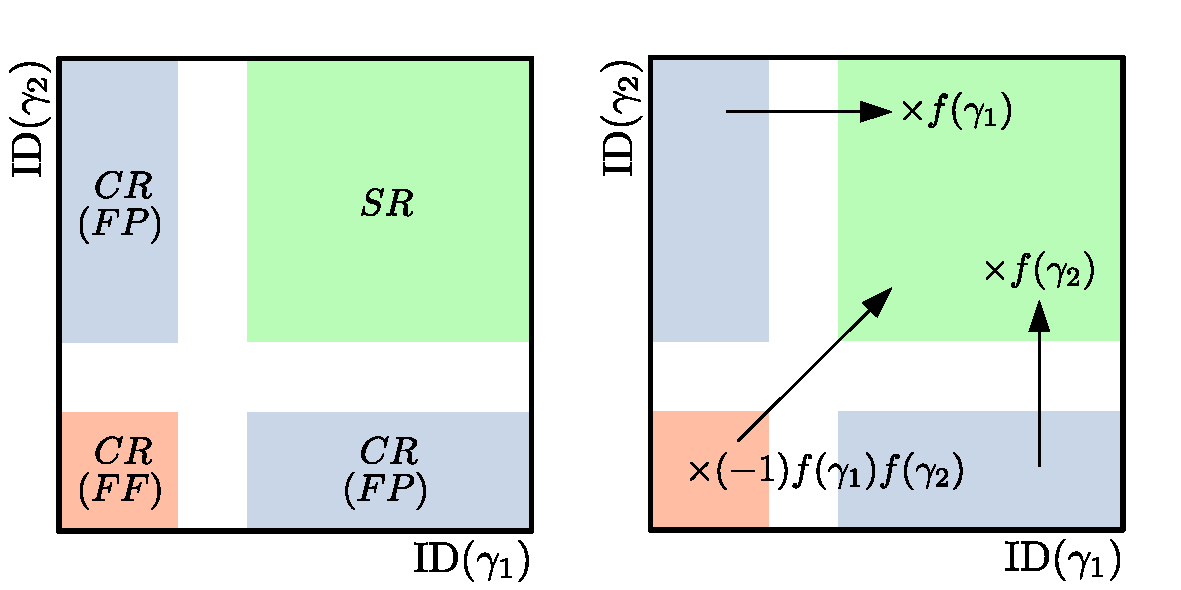
\includegraphics[width=.8\textwidth]{Figures/hgg_overview/dijetbdt_illustration.pdf}
  \caption[Illustration of the data-driven background estimate method for the dijet BDT]
  {
    A schematic showing the application of transfer factors to estimate the fake component of the background in the signal region (SR) directly from data events in dedicated control regions (CR).
  }
  \label{fig:dijetbdt_transferfunctions}
\end{figure}

\begin{figure}
  \centering
  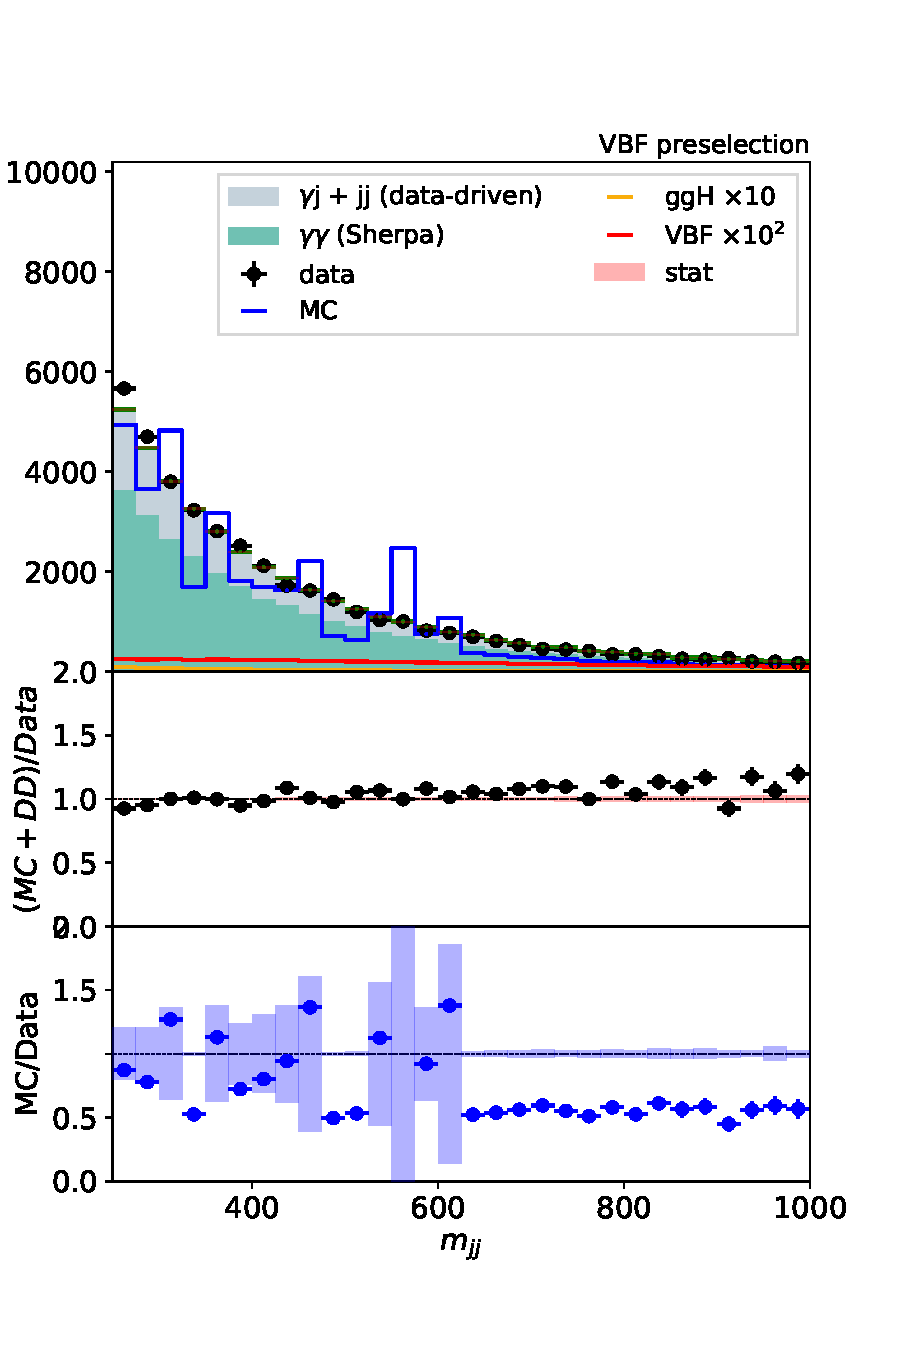
\includegraphics[width=.375\textwidth]{Figures/hgg_overview/DijetBDT_input_Mjj.pdf}
%   \hfill
  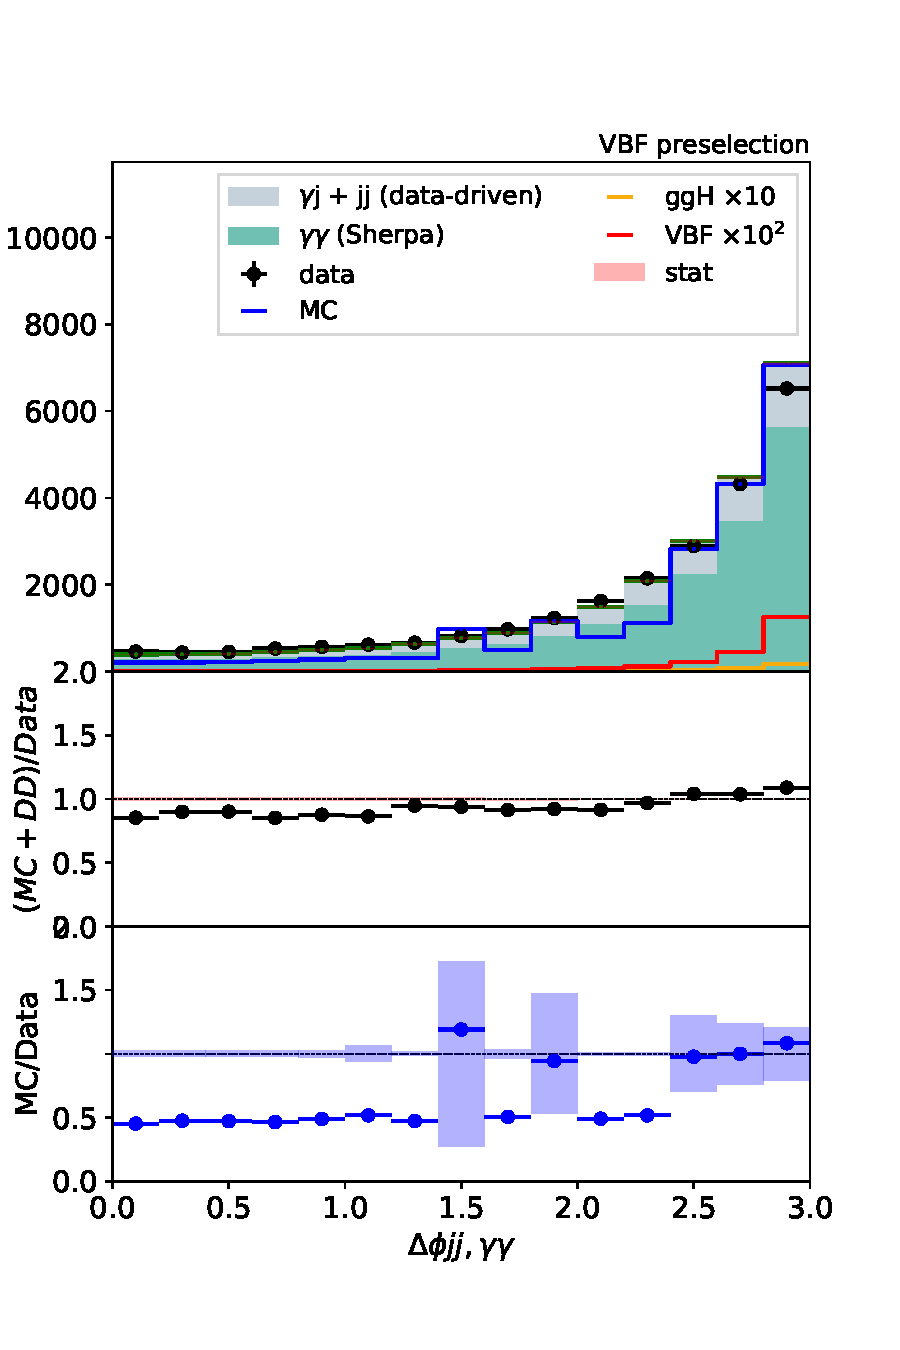
\includegraphics[width=.375\textwidth]{Figures/hgg_overview/DijetBDT_input_dPhi.pdf}
  \vspace{-.5cm}
  \caption[Dijet BDT input features using the data-driven background estimate]
  {
    Input features to the dijet BDT: \mjj and $\Delta\phi_{jj,\gamma\gamma}$. The data events shown by the black points were collected in the 2018 period. The simulated $\gamma\gamma$ background estimate and the data-driven $\gamma$+jet and jet+jet background estimates are shown by the filled green and blue histograms, respectively. In addition, the simulated $\gamma$+jet and jet+jet background estimate is shown by the blue line. The bottom panel shows the ratio of the purely simulated background estimate to data, where the agreement clearly suffers from a lack of MC statistics in the $\gamma$+jet and jet+jet component of the background. The middle panel shows the ratio including the data-driven estimate of the background, where the agreement is much improved.
  }
  \label{fig:dijetbdt_validation}
\end{figure}


Figure \ref{fig:dijetbdt_outputs} shows the two independent output probabilities of the dijet BDT: the VBF probability, $p_{\rm{VBF}}$ (left), and the ggH probability, $p_{\rm{ggH}}$ (right). The background probability is simply realised according to the equation: $p_{\rm{bkg}}=1-p_{\rm{VBF}}-p_{\rm{ggH}}$. 

\begin{figure}
  \centering
  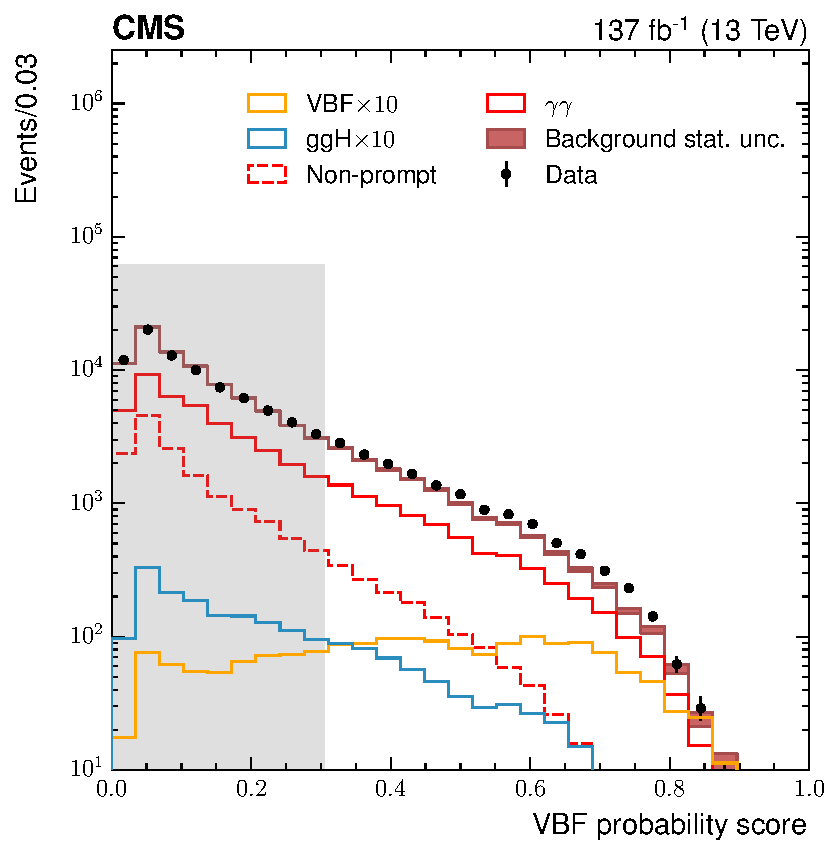
\includegraphics[width=.4\textwidth]{Figures/hgg_overview/DijetBDT_DD_vbfMvaResult_prob_VBF_logPlot.pdf}
  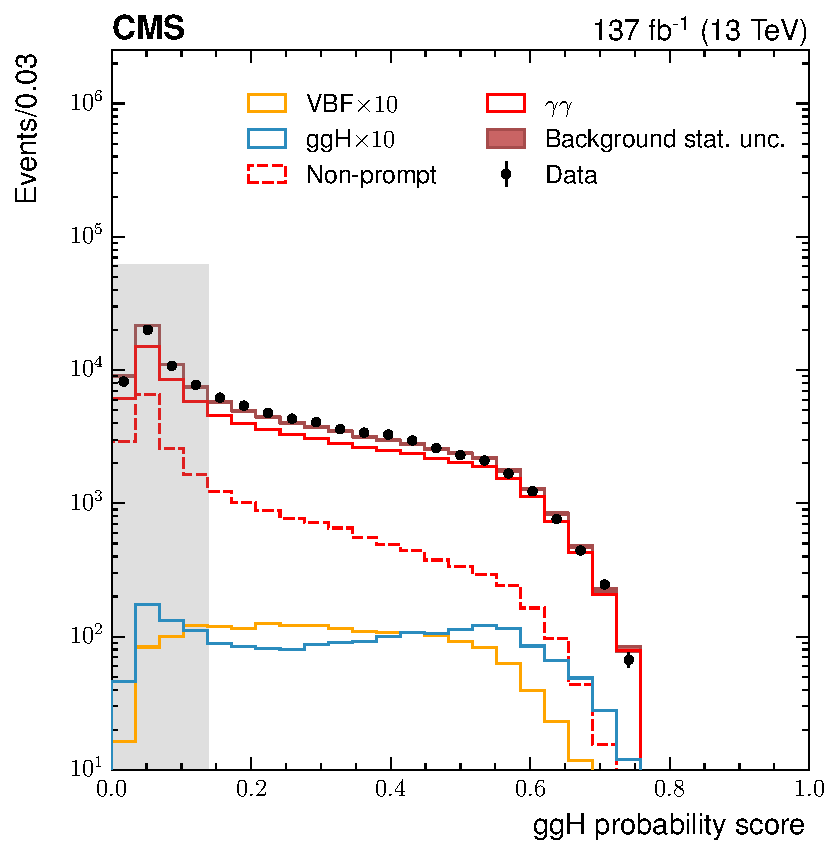
\includegraphics[width=.4\textwidth]{Figures/hgg_overview/DijetBDT_ggHprob.pdf}
  \caption[Dijet BDT output probabilities: $p_{\rm{VBF}}$ and $p_{\rm{ggH}}$]
  {
    The dijet BDT output probabilities, $p_{\rm{VBF}}$ (left) and $p_{\rm{ggH}}$ (right), for events with an invariant mass in the range $100<\mgg<180$~GeV, passing the VBF-like signal region selection. Data events are shown by the black points, and the corresponding background simulation with statistical uncertainty is shown by the red band. The components of the background are plotted in separate histograms in red. In addition the orange and blue histograms show the simulated VBF and ggH signal events, respectively. The shaded grey regions contain $p_{\rm{VBF}}$ values below the lowest threshold used to define the VBF production tags, and $p_{\rm{ggH}}$ values below the lowest threshold used to define the ggH VBF-like tags. The full data set collected in the period 2016-2018 and the corresponding simulation is shown.
  }
  \label{fig:dijetbdt_outputs}
\end{figure}

The VBF-like global category is split to target different kinematic bins of the STXS framework. For the qqH STXS bins, events are assigned to one of five regions using the reconstructed equivalents of the truth-level variables. Firstly, the qqH BSM STXS bin ($p_T^H>200$~GeV) is targeted by requiring the reconstructed $p_T^{\gamma\gamma}>200$~GeV. The four remaining VBF-like bins are targeted according to a boundary in the reconstructed $m_{jj}$ at 700~GeV, and a boundary in the transverse momentum of the dijet-plus-diphoton system, $p_T^{\gamma\gamma jj}$, at 25~GeV. In each region, two tags are constructed by placing optimised boundaries on the dijet-BDT output probabilities. This optimisation considers VBF production as signal and groups ggH production with other background events. In this manner, a lower bound is placed on $p_{\rm{VBF}}$, and an upper bound is placed on $p_{\rm{ggH}}$. On top of this, the optimisation procedure includes a threshold on the diphoton BDT score to further reduce the number of background events.

Events failing the above criteria are then considered for an additional two tags, designed to be enriched in events from the four ggH VBF-like bins. This optimisation considers ggH as signal, and VBF as background. This amounts to placing a lower bound on $p_{\rm{ggH}}$ and an upper bound on $p_{\rm{VBF}}$, in addition to a lower threshold on the diphoton BDT score. Events with $p_T^{\gamma\gamma}>200$~GeV that have failed the qqH BSM selection criteria are not considered in the ggH VBF-like tags as they are specifically targeted further down the priority sequence by the ggH BSM analysis categories.

\subsubsection{VH hadronic topology}
VH hadronic events enrich a single STXS bin (qqH VH-like) in the EW qqH scheme. This is defined at truth-level with the requirement, $60<m_{jj}<120$~GeV, to be consistent with a dijet system originating from the decay of a vector boson. To target this bin, an orthogonal signal region is defined with a different selection on the reconstructed dijet-system: events are required to have two jets within $|\eta^j|<2.4$ and with $p_T^j>30$~GeV, satisfying the same pileup-identification BDT and photon-ID BDT score requirements as the VBF-topology signal region, with a reconstructed $m_{jj}$ between 60 and 120~GeV. 

\begin{figure}
  \centering
  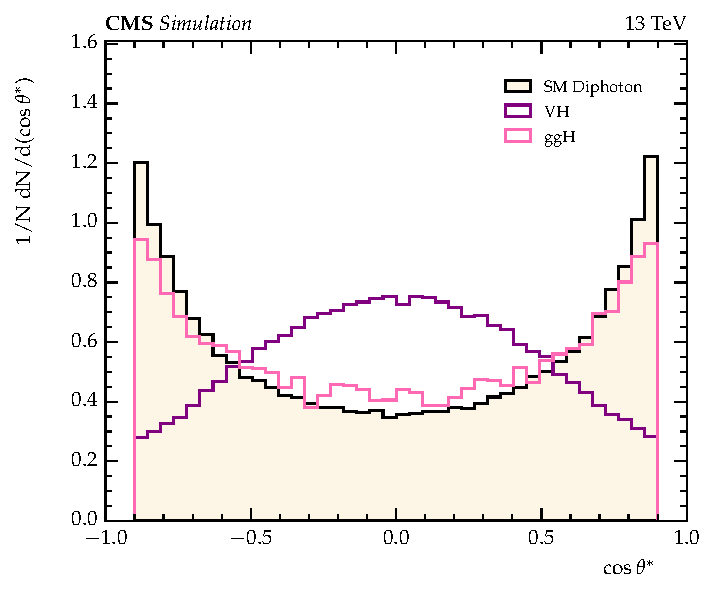
\includegraphics[width=.49\textwidth]{Figures/hgg_overview/cosThetaStar.pdf}
  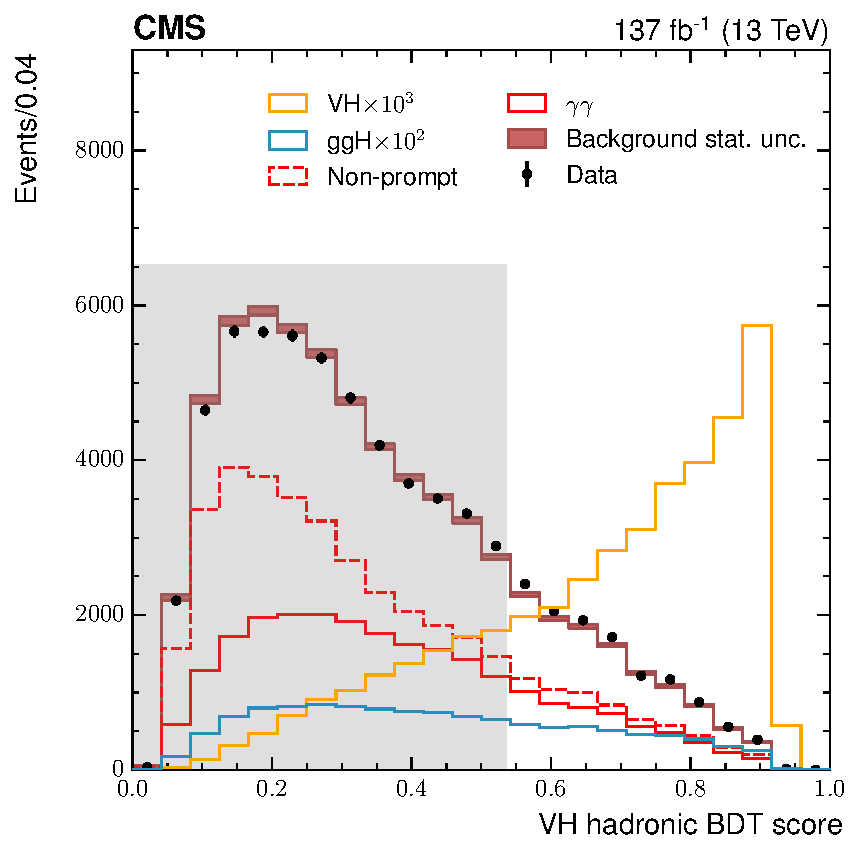
\includegraphics[width=.49\textwidth]{Figures/hgg_overview/VHhadBDT_DD_VH_had_mvascore_no_stack.pdf}
  \caption[VH hadronic BDT output score]
  {
    Distribution of the $\cos{\theta^*}$ variable for simulated VH, ggH, and SM-diphoton production events (left). The output score for the VH hadronic BDT (right), for events with an invariant mass in the range $100<\mgg<180$~GeV, passing the VH-like signal region selection. Data events are shown by the black points, and the corresponding background simulation with statistical uncertainty is shown by the red band. The components of the background are plotted in separate histograms in red. In addition the orange and blue histograms show the simulated VH and ggH signal events, respectively. The shaded grey region illustrates the lowest threshold used to define the VH hadronic analysis categories, The full data set collected in the period 2016-2018 and the corresponding simulation is shown.
  }
  \label{fig:categorisation_vhhad}
\end{figure}

The VH hadronic BDT is then trained to isolate VH signal events, and subsequently reduce the contribution from ggH and other background processes in the signal region. One of the key input features which helps identify dijets consistent with a vector boson decay is the $\cos{\theta^*}$ variable, where $\theta^*$ is the angle that the diphoton system makes in the diphoton-dijet centre-of-mass frame, with respect to the direction of motion of the diphoton-dijet system in the lab frame. The distribution of this variable is reasonably uniform for VH events, while it is strongly peaked at $\pm$1 for background and ggH events, as shown in Figure~\ref{fig:categorisation_vhhad}~(left). To train the BDT, the VH, ggH, and SM diphoton samples are taken from simulation, whereas the background with jets faking photons is again derived from a data control region, in an analogous manner to that used for the dijet BDT. The output score for the VH hadronic BDT is shown in Figure~\ref{fig:categorisation_vhhad}~(right). Two analysis tags are defined by placing optimised boundaries on both the VH hadronic BDT and diphoton BDT output scores. 

% \begin{figure}
%   \centering
%   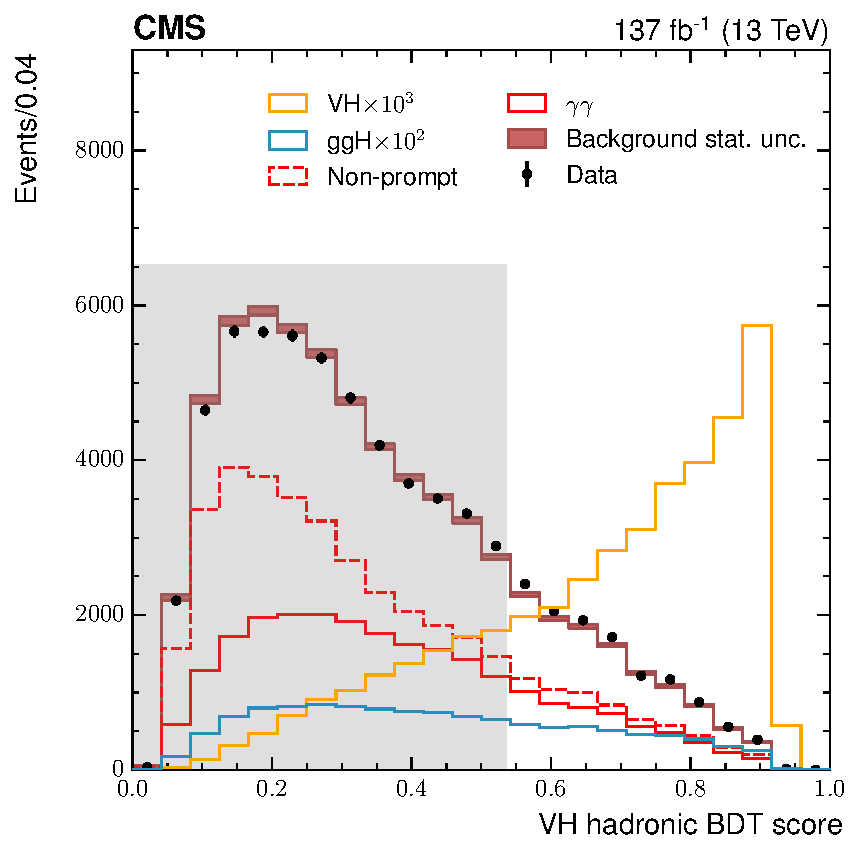
\includegraphics[width=.5\textwidth]{Figures/hgg_overview/VHhadBDT_DD_VH_had_mvascore_no_stack.pdf}
%   \caption[VH hadronic BDT output score]
%   {
%     The output score for the VH hadronic BDT, for events with an invariant mass in the range $100<\mgg<180$~GeV, passing the VH-like signal region selection. Data events are shown by the black points, and the corresponding background simulation with statistical uncertainty is shown by the red band. The components of the background are plotted in separate histograms in red. In addition the orange and blue histograms show the simulated VH and ggH signal events, respectively. The shaded grey region illustrates the lowest threshold used to define the VH hadronic analysis categories, The full data set collected in the period 2016-2018 and the corresponding simulation is shown.
%   }
%   \label{fig:categorisation_vhhad}
% \end{figure}

Table \ref{tab:qqH_category_yields} provides a summary of the expected signal and background yields in each of the analysis categories described in this section: those targeting the VBF-topology from both the ggH and qqH production modes, and the VH hadronic topology. The final set of analysis categories described in this section, along with their targeted STXS bin (or bins), are shown in Figure~\ref{fig:qqH_categorisation_schematic}.

\begin{table}
    \caption[Expected yields for the qqH production mode categories]{The expected number of events for $m_{\rm{H}}=125$~GeV in the analysis categories targeting the EW qqH STXS regions, in addition to the two tags targeting ggH production with a VBF-like topology, shown for an integrated luminosity of 137~\fbinv. The fraction of the total number of events arising from each production mode in each analysis category is provided, as is the fraction of events originating from the targeted STXS bin (or bins). Here, ggH includes contributions from the sub-dominant ggZ(q$\bar{\rm{q}}$)H and bbH production modes, and ``Top" represents both ttH and tH production together. The $\sigma_{\rm{eff}}$, defined as the smallest interval containing 68.3\% of the $m_{\gamma\gamma}$ distribution provides an indication of the mass resolution in each category. Also provided are the estimated number of background events-per-GeV in the signal peak region, the quantity $F_{68}=S_{68}/(S_{68}+B_{68})$, where $S_{68}$ and $B_{68}$ are the expected number of signal and background events in a $\pm1\sigma_{\rm{eff}}$ window centred on $m_{\rm{H}}$, respectively, and the approximate significance, $Z_{68}=S_{68}/\sqrt{S_{68}+B_{68}}$. The final column shows the significance for the targeted STXS bin (or bins) only, $Z^{\rm{target}}_{68}$,  where other Higgs boson signal events are considered as background.}
    \label{tab:qqH_category_yields}
    % \vspace{.5cm}
    \centering
    \scriptsize
    \renewcommand{\arraystretch}{1.1}
    \setlength{\tabcolsep}{3pt}
    \hspace*{-5cm}
    \begin{tabular}{l|cccccccc|c|ccc}
    \multirow{3}{*}{Analysis categories} & \multicolumn{8}{c|}{SM 125 GeV Higgs boson expected signal} & \multirow{3}{*}{\begin{tabular}[c]{@{}c@{}}Bkg\\(GeV$^{\rm{-1}}$)\end{tabular}} & \multirow{3}{*}{$F_{68}$} & \multirow{3}{*}{$Z_{68}$} & \multirow{3}{*}{$Z^{\rm{target}}_{68}$} \\
     & \multirow{2}{*}{Total} & \multirow{2}{*}{\begin{tabular}[c]{@{}c@{}}Target\\STXS bin(s)\end{tabular}} & \multicolumn{5}{c}{Fraction of total events} & \multirow{2}{*}{\begin{tabular}[c]{@{}c@{}}$\sigma_{\rm{eff}}$\\(GeV)\end{tabular}} & & & & \\
     & & & ggH & VBF & VH had & VH lep & Top & & & & & \\ \hline
     ggH VBF-like Tag0 & 14.1 & 37.7\% & 65.9\% & 27.3\% & 3.8\% & 0.8\% & 2.3\% & 1.85 & 35 & 0.13 & 1.09 & 0.41 \\
     ggH VBF-like Tag1 & 32.5 & 30.2\% & 61.3\% & 29.8\% & 4.1\% & 1.1\% & 3.7\% & 1.83 & 117 & 0.09 & 1.39 & 0.42 \\
     [\cmsTabSkip]
     qqH low $\mjj$ low $\ptHjj$ Tag0 & 17.2 & 48.2\% & 36.6\% & 62.6\% & 0.4\% & 0.1\% & 0.3\% & 1.89 & 26 & 0.19 & 1.48 & 0.71 \\
     qqH low $\mjj$ low $\ptHjj$ Tag1 & 13.5 & 48.5\% & 35.5\% & 63.4\% & 0.6\% & 0.1\% & 0.3\% & 1.74 & 24 & 0.18 & 1.27 & 0.62 \\
     [\cmsTabSkip]
     qqH high $\mjj$ low $\ptHjj$ Tag0 & 27.0 & 70.4\% & 17.1\% & 82.7\% & 0.2\% & - & 0.1\% & 1.78 & 11 & 0.48 & 2.94 & 2.07 \\
     qqH high $\mjj$ low $\ptHjj$ Tag1 & 12.9 & 58.2\% & 20.8\% & 78.7\% & 0.3\% & 0.1\% & 0.2\% & 1.99 & 13 & 0.25 & 1.48 & 0.86 \\
     [\cmsTabSkip]
     qqH low $\mjj$ high $\ptHjj$ Tag0 & 10.4 & 15.0\% & 56.0\% & 41.3\% & 1.3\% & 0.4\% & 1.0\% & 1.92 & 27 & 0.12 & 0.90 & 0.14 \\
     qqH low $\mjj$ high $\ptHjj$ Tag1 & 20.2 & 17.0\% & 57.9\% & 36.9\% & 2.4\% & 0.7\% & 2.1\% & 1.74 & 94 & 0.08 & 1.01 & 0.17 \\
     [\cmsTabSkip]
     qqH high $\mjj$ high $\ptHjj$ Tag0 & 18.1 & 25.6\% & 28.1\% & 70.8\% & 0.4\% & 0.1\% & 0.5\% & 1.88 & 17 & 0.27 & 1.82 & 0.47 \\
     qqH high $\mjj$ high $\ptHjj$ Tag1 & 17.5 & 23.8\% & 39.5\% & 57.8\% & 0.9\% & 0.3\% & 1.5\% & 1.98 & 42 & 0.12 & 1.20 & 0.29 \\
     [\cmsTabSkip]
     qqH BSM Tag0 & 11.2 & 71.2\% & 24.4\% & 74.8\% & 0.1\% & 0.1\% & 0.6\% & 1.62 & 3.9 & 0.54 & 2.02 & 1.44 \\
     qqH BSM Tag1 & 6.8 & 56.4\% & 36.9\% & 59.9\% & 1.1\% & 0.4\% & 1.7\% & 1.67 & 4.6 & 0.37 & 1.31 & 0.74 \\
     [\cmsTabSkip]
     qqH VH-like Tag0 & 16.3 & 55.8\% & 36.5\% & 2.8\% & 55.0\% & 1.4\% & 4.2\% & 1.72 & 20 & 0.24 & 1.64 & 0.91 \\
     qqH VH-like Tag1 & 47.1 & 26.8\% & 64.9\% & 4.7\% & 26.4\% & 1.2\% & 2.9\% & 1.66 & 135 & 0.12 & 1.97 & 0.53 \\
     [\cmsTabSkip]
\end{tabular}

    \hspace*{-5cm}
\end{table}

\subsection{VH leptonic categorisation}
\begin{figure}
  \centering
  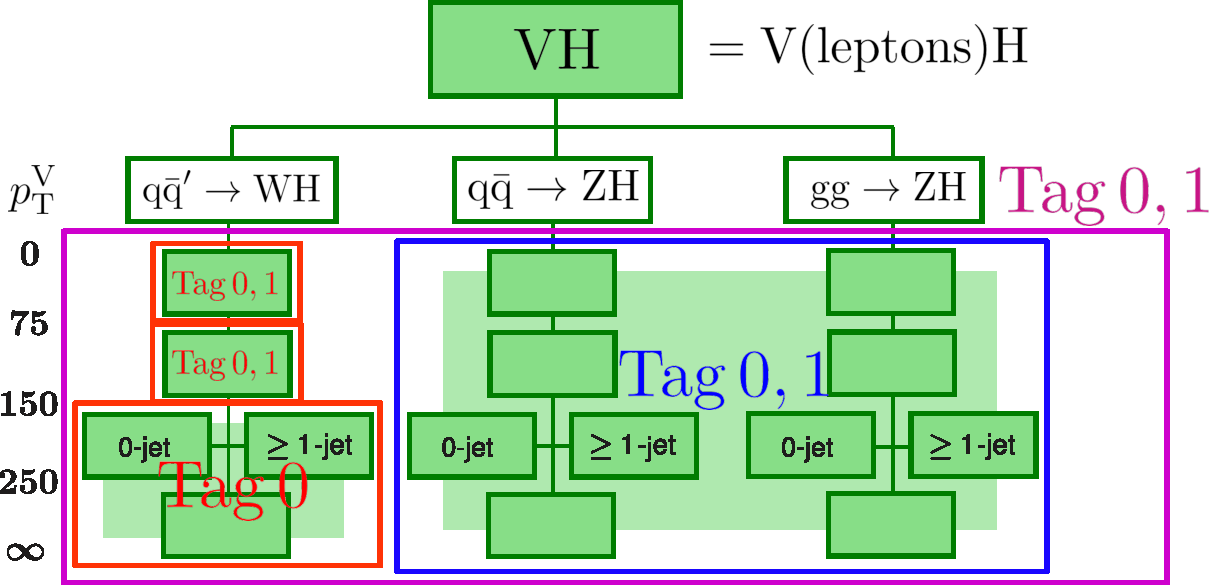
\includegraphics[width=.8\textwidth]{Figures/hgg_overview/categorisation_schematics/VHlepCategorisation.pdf}
  \caption[VH leptonic categorisation schematic]
  {
    A schematic of the VH leptonic categorisation scheme. The WH leptonic, ZH leptonic and VH MET analysis categories are defined by the red, blue, and purple boxes, respectively. The analysis categories surround the targeted STXS bin (or bins). The number of tags for each analysis region are highlighted in the plot.
  }
  \label{fig:VHlep_categorisation_schematic}
\end{figure}

Three global categories are constructed to target Higgs boson production in association with a leptonically-decaying vector boson. These categories are orthogonal to each other by construction due to requiring a different number of isolated charged leptons in the event: two for ZH leptonic, one for WH leptonic and zero for the VH MET category. The ZH leptonic category imposes a requirement on the dilepton invariant mass, $m_{ll}$, to be between 60 and 120~GeV. This ensures the two leptons are consistent with originating from the decay of a Z boson: Z($\rightarrow\ell\ell$)H. The WH leptonic category, which targets W($\rightarrow\ell\nu$)H production, places additional requirements on the photon-ID BDT score to further reject backgrounds from jets faking photons, and on the invariant mass of the reconstructed lepton with each photon to reduce the contribution from the Drell-Yan background in which an electron has been misidentified as a photon. The VH MET category is constructed to target events from Z($\rightarrow\nu\nu$)H production, and W($\rightarrow\ell\nu)$H production where the charged lepton is not reconstructed in the detector. Here, events are required to have $\met>50$~GeV and the azimuthal angle between \metv and the diphoton system must be greater than two radians. The categories targeting VH leptonic production are placed between the ttH leptonic and ttH hadronic global categories in the priority sequence.

To further distinguish between VH leptonic signal and background events, a BDT is trained in each global category; the details of which are provided in Table \ref{tab:categorisation_discriminants}. The simulated background processes include SM diphoton production, $\gamma$+jets, Drell-Yan, diboson production, and tt production. In addition, the Higgs boson production modes other than VH are treated as backgrounds. Due to the large contamination of the $\gamma$+jet events in the VH MET category, a data-driven approach is used to estimate this component of the background. The precise details of this approach are described in more detail in the context of the dijet BDT in the previous section. Figure \ref{fig:categorisation_vhlep} shows the output scores of the VH leptonic BDTs.

The WH leptonic category is sensitive to three kinematic regions in the STXS framework. Boundaries are placed on the reconstructed \ptgg at 75 and 150~GeV, to target the equivalent truth-level splittings in the $p_T^V$ variable. Note, the reconstructed \ptgg provides the best handle on the truth-level $p_T^V$, since the presence of a neutrino in the final-state means that the vector boson cannot be fully reconstructed. No splitting of the ZH leptonic or the VH MET categories is performed. The final analysis categories are constructed by placing optimised boundaries on the respective BDT output scores. In total, two tags are defined for ZH leptonic, five for WH leptonic (two for both the $\ptgg<75$~GeV and $75<\ptgg<150$~GeV regions, and one for the $\ptgg>150$~GeV region), and three for VH MET. This set of analysis categories are shown in the schematic in Figure~\ref{fig:VH_categorisation_schematic}. The expected signal and background yields for the categories targeting VH leptonic production are shown in Table \ref{tab:vhlep_category_yields}.

\begin{figure}
  \centering
  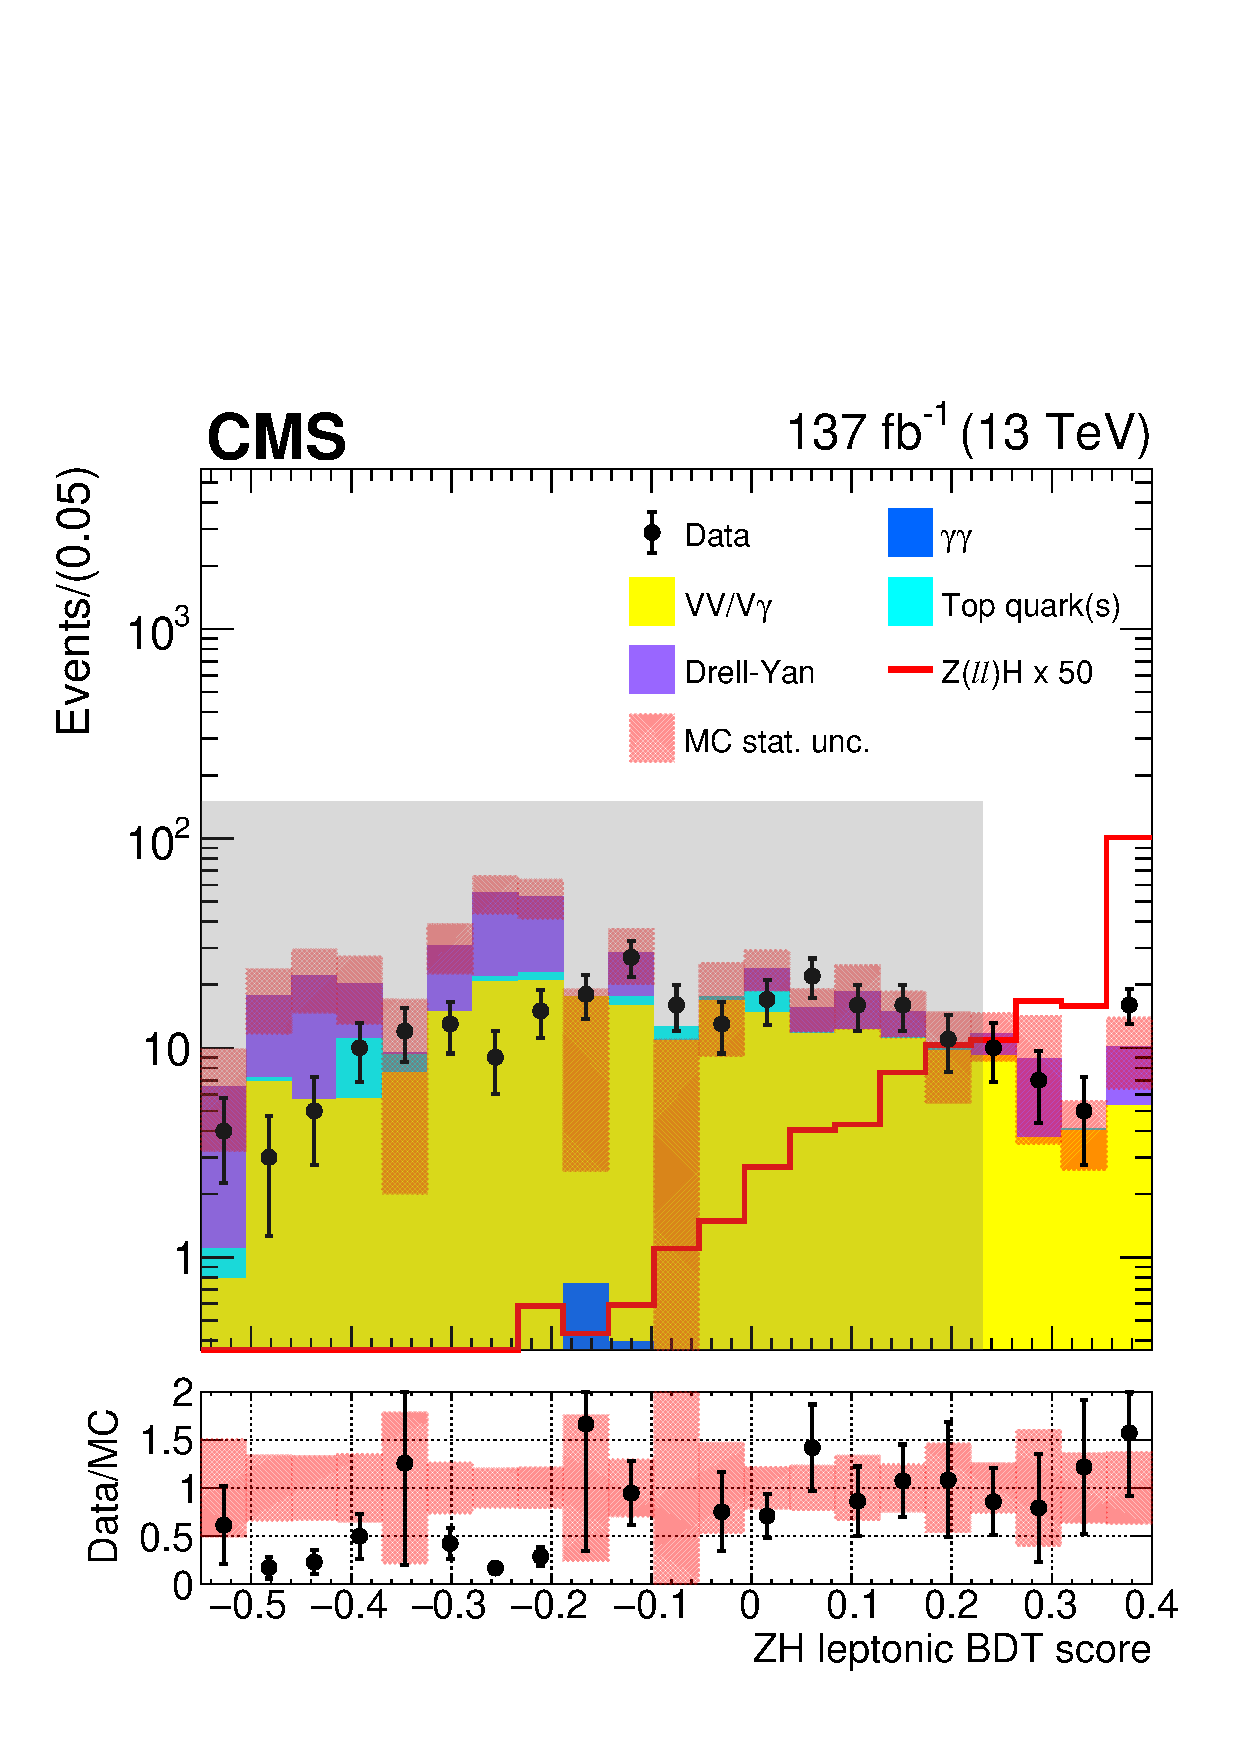
\includegraphics[width=.32\textwidth]{Figures/hgg_overview/ZHMVA.pdf}
  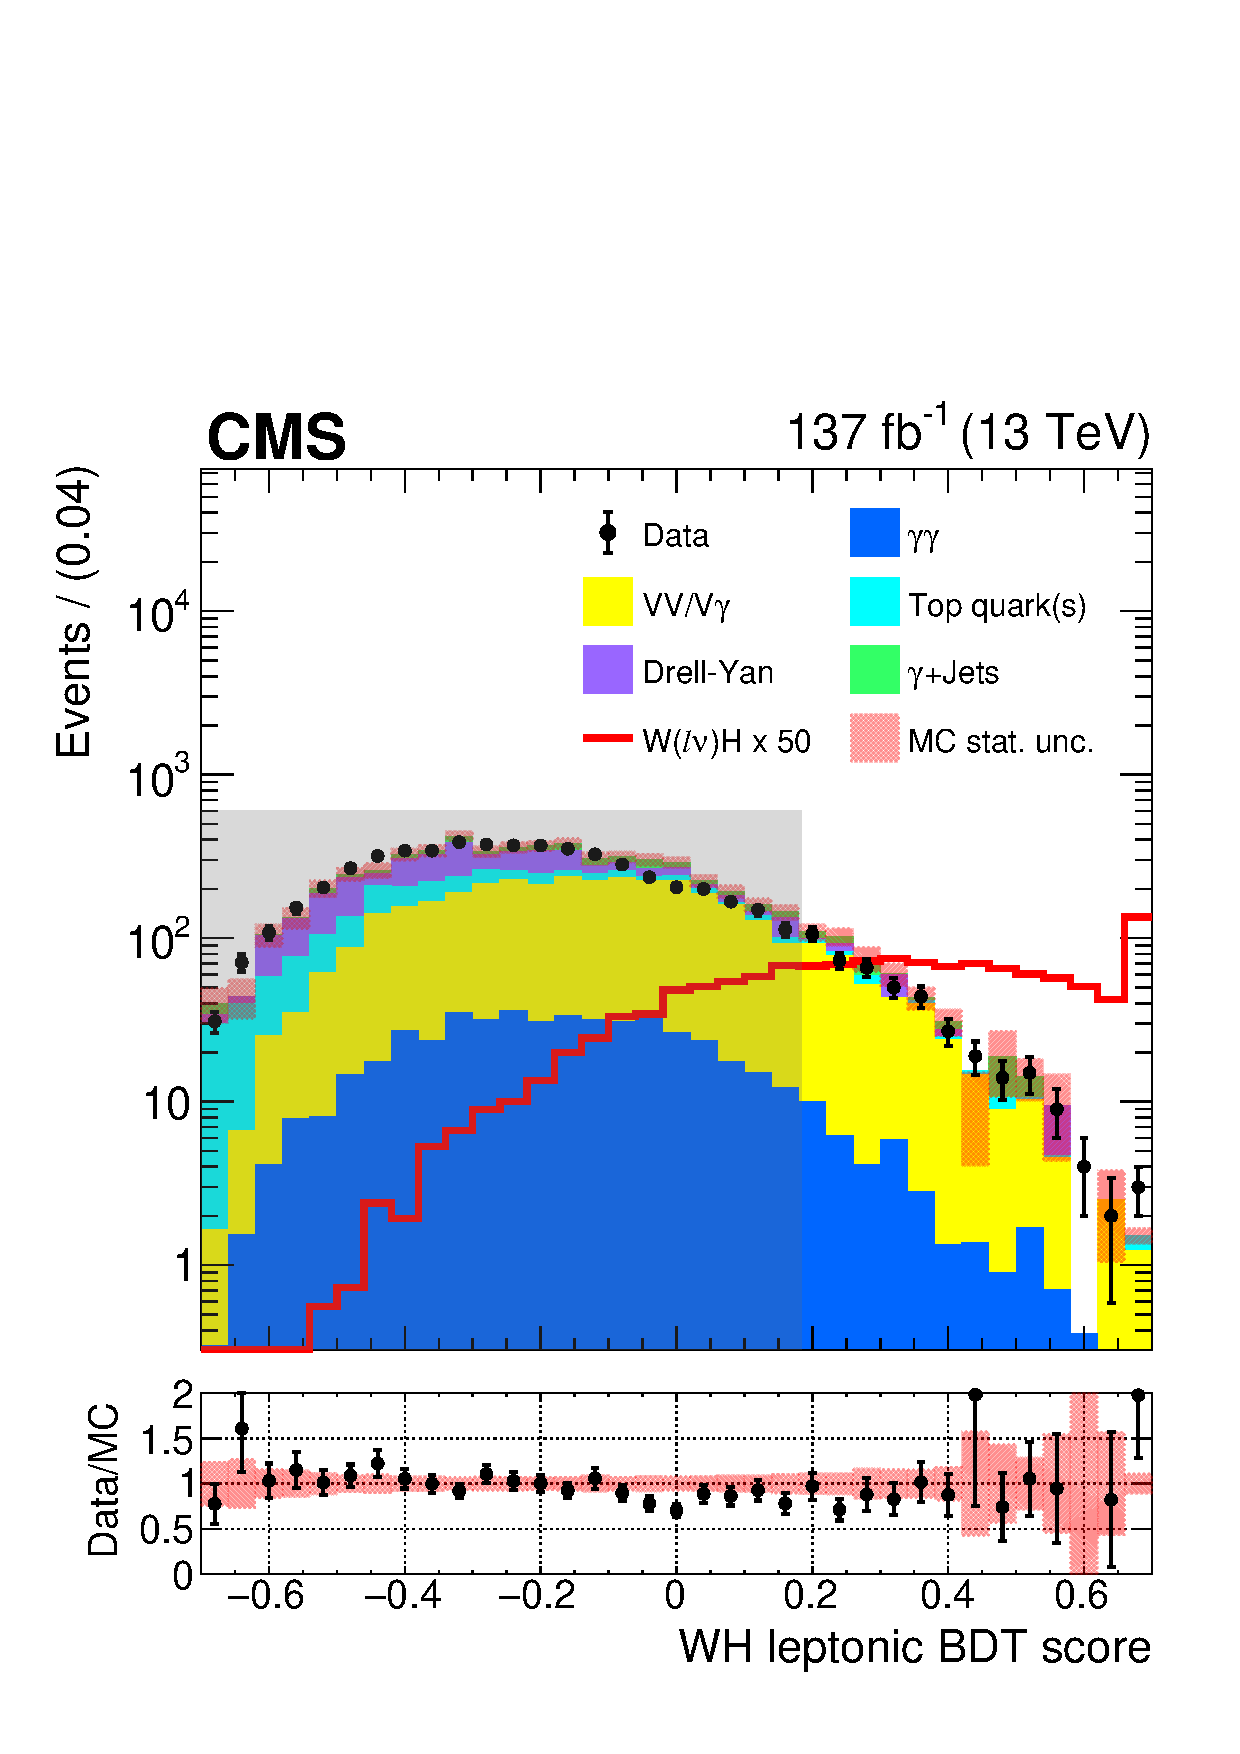
\includegraphics[width=.32\textwidth]{Figures/hgg_overview/WHMVA.pdf}
  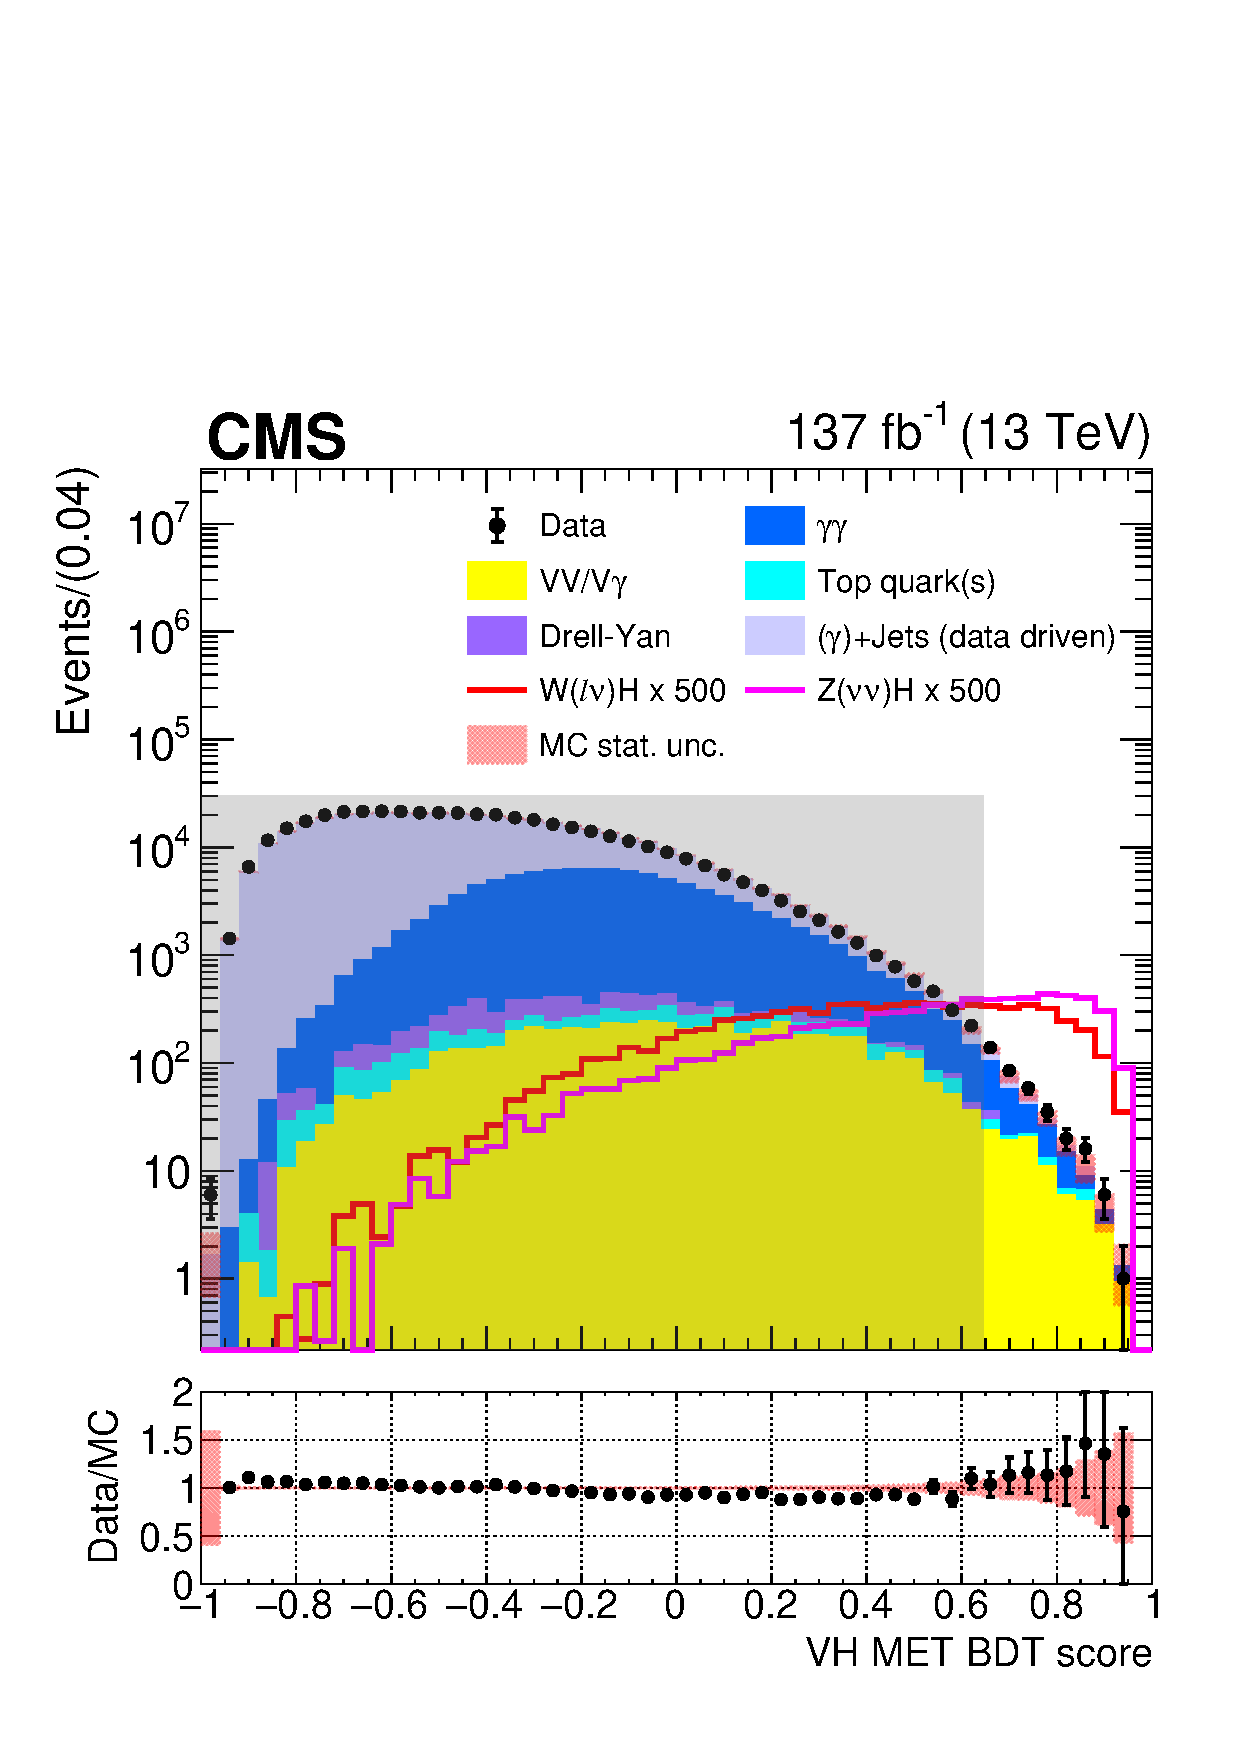
\includegraphics[width=.32\textwidth]{Figures/hgg_overview/VHMETMVA.pdf}
  \caption[Output scores of the discriminants used for the VH leptonic production mode categories]
  {
    Distributions of the ZH leptonic (left), WH leptonic (centre) and VH MET (right) BDT output scores, for both data (black points) and simulated signal and background events (histograms). For the VH MET BDT, the $\gamma$+jet component of the background is derived directly from data. The statistical uncertainty in the data (simulation) is shown by the black error bars (shaded pink band). Events in the regions shaded grey are not considered for the VH leptonic categories. 
    %The signal components have been scaled by 50, 50, and 500 for the ZH leptonic, WH leptonic, and VH MET BDT distributions respectively. 
    The full data set collected in the period 2016-2018 and the corresponding simulation is shown.
  }
  \label{fig:categorisation_vhlep}
\end{figure}

\begin{table}
    \caption[Expected yields for the VH leptonic production mode categories]{The expected number of events for $m_{\rm{H}}=125$~GeV in the analysis categories targeting the VH leptonic production modes, shown for an integrated luminosity of 137~\fbinv. The fraction of the total number of events arising from each production mode in each analysis category is provided, as is the fraction of events originating from the targeted STXS bin (or bins). Here, ggH includes contributions from the sub-dominant ggZ(q$\bar{\rm{q}}$)H and bbH production modes, qqH includes both VBF and V(q$\bar{\rm{q}}$)H production, and ``Top" represents both ttH and tH production together. The $\sigma_{\rm{eff}}$, defined as the smallest interval containing 68.3\% of the $m_{\gamma\gamma}$ distribution provides an indication of the mass resolution in each category. Also provided are the estimated number of background events-per-GeV in the signal peak region, the quantity $F_{68}=S_{68}/(S_{68}+B_{68})$, where $S_{68}$ and $B_{68}$ are the expected number of signal and background events in a $\pm1\sigma_{\rm{eff}}$ window centred on $m_{\rm{H}}$, respectively, and the approximate significance, $Z_{68}=S_{68}/\sqrt{S_{68}+B_{68}}$. The final column shows the significance for the targeted STXS bin (or bins) only, $Z^{\rm{target}}_{68}$,  where other Higgs boson signal events are considered as background.}
    \label{tab:vhlep_category_yields}
    % \vspace{.5cm}
    \centering
    \scriptsize
    \renewcommand{\arraystretch}{1}
    \setlength{\tabcolsep}{3pt}
    \hspace*{-1.5cm}
    \begin{tabular}{l|ccccccccc|c|ccc}
    \multirow{3}{*}{Analysis categories} & \multicolumn{9}{c|}{SM 125 GeV Higgs boson expected signal} & \multirow{3}{*}{\begin{tabular}[c]{@{}c@{}}Bkg\\(GeV$^{\rm{-1}}$)\end{tabular}} & \multirow{3}{*}{$F_{68}$} & \multirow{3}{*}{$Z_{68}$} & \multirow{3}{*}{$Z^{\rm{target}}_{68}$} \\
     & \multirow{2}{*}{Total} & \multirow{2}{*}{\begin{tabular}[c]{@{}c@{}}Target\\STXS bin(s)\end{tabular}} & \multicolumn{6}{c}{Fraction of total events} & \multirow{2}{*}{\begin{tabular}[c]{@{}c@{}}$\sigma_{\rm{eff}}$\\(GeV)\end{tabular}} & & & & \\
     & & & ggH & qqH & WH lep & ZH lep & ggZH lep & Top & & & & & \\ \hline
     ZH lep Tag0 & 2.4 & 99.6\% & - & - & - & 82.0\% & 17.7\% & 0.4\% & 1.67 & 0.74 & 0.57 & 0.97 & 0.97 \\
     ZH lep Tag1 & 0.9 & 97.5\% & 0.1\% & - & 0.2\% & 80.7\% & 16.9\% & 2.2\% & 1.85 & 0.74 & 0.30 & 0.43 & 0.41 \\
     [\cmsTabSkip]
     WH lep $p_{T}^{V}<75$ Tag0 & 2.0 & 81.1\% & - & 0.2\% & 95.0\% & 3.3\% & 0.2\% & 1.3\% & 1.89 & 0.99 & 0.42 & 0.75 & 0.61 \\
     WH lep $p_{T}^{V}<75$ Tag1 & 4.5 & 75.7\% & 2.6\% & 0.5\% & 87.2\% & 7.0\% & 0.3\% & 2.4\% & 1.85 & 7.5 & 0.18 & 0.74 & 0.56 \\
     [\cmsTabSkip]
     WH lep $75<p_{T}^{V}<150$ Tag0 & 3.0 & 77.7\% & 0.7\% & 0.3\% & 93.2\% & 3.4\% & 0.8\% & 1.6\% & 1.94 & 0.89 & 0.54 & 1.04 & 0.81 \\
     WH lep $75<p_{T}^{V}<150$ Tag1 & 3.3 & 60.8\% & 1.7\% & 1.4\% & 83.1\% & 7.7\% & 1.6\% & 4.4\% & 2.02 & 2.4 & 0.31 & 0.83 & 0.51 \\
     [\cmsTabSkip]
     WH lep $p_{T}^{V}>150$ Tag0 & 3.5 & 79.9\% & 0.5\% & 0.4\% & 91.5\% & 3.6\% & 1.1\% & 2.8\% & 1.84 & 0.33 & 0.80 & 1.37 & 1.10 \\
     [\cmsTabSkip]
     VH MET Tag0 & 2.2 & 97.9\% & 0.4\% & 0.9\% & 23.5\% & 56.9\% & 17.6\% & 0.8\% & 2.22 & 0.78 & 0.46 & 0.84 & 0.82 \\
     VH MET Tag1 & 3.6 & 90.5\% & 4.6\% & 3.1\% & 28.8\% & 46.0\% & 15.7\% & 1.9\% & 2.30 & 2.2 & 0.33 & 0.89 & 0.81 \\
     VH MET Tag2 & 6.6 & 72.2\% & 15.5\% & 8.8\% & 27.7\% & 33.5\% & 11.0\% & 3.5\% & 2.15 & 10 & 0.17 & 0.87 & 0.63 \\
     [\cmsTabSkip]
\end{tabular}
    \hspace*{-1.5cm}
\end{table}

\subsection{Top-associated categorisation}\label{sec:top_categorisation}
\begin{figure}
  \centering
  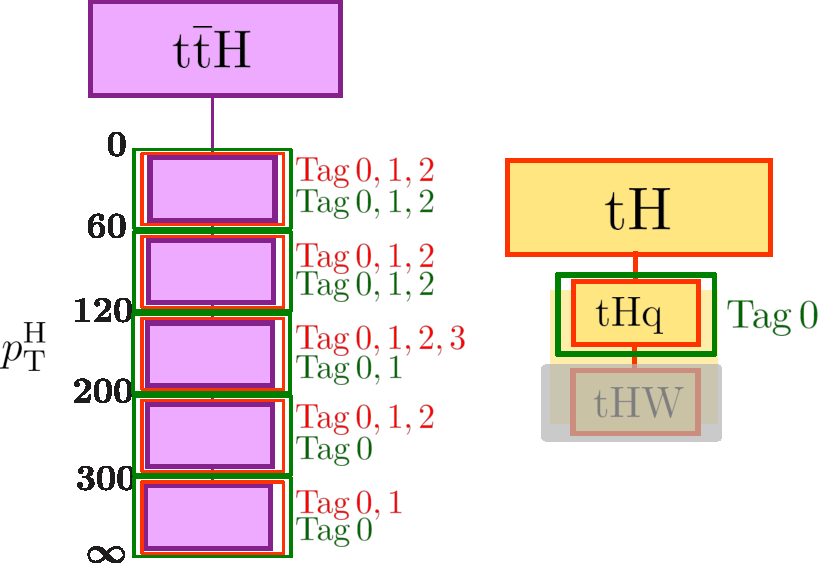
\includegraphics[width=.6\textwidth]{Figures/hgg_overview/categorisation_schematics/TopSchematic.pdf}
  \caption[Top-associated categorisation schematic]
  {
    A schematic of the top-associated categorisation scheme. The hadronic and leptonic analysis categories are defined by the red and green boxes, respectively. The analysis categories surround the targeted STXS bin (or bins). The number of tags for each analysis region are highlighted in the plot. The shaded-grey region indicates there is no analysis category explicitly targeting the tHW production mode.
  }
  \label{fig:top_categorisation_schematic}
\end{figure}
The two global categories with the highest priority in the sequence are constructed to be enriched with events from the tHq and ttH production modes, where at least one top quark in the event decays leptonically. In both, events are required to have at least one isolated charged lepton, as well as one or more jets. Moreover, the tHq leptonic selection requires an additional jet, tagged as originating from the hadronisation of a b quark. 

Due to their similar final-state topology, a dedicated deep neural network, referred to as the Top DNN, is trained to differentiate between the tHq and ttH production modes. Figure \ref{fig:categorisation_top} (top left) shows the output score of the Top DNN for tHq, ttH and the relevant SM background processes. A requirement is placed on this score in both the tHq leptonic and ttH leptonic categories to minimise the contamination from the opposing production mode. An additional discriminant is then trained in each global category using simulated events to reduce the contamination from other non-Higgs boson background processes. The simulated backgrounds include tt+$\gamma\gamma$, tt+$\gamma$+jet, tt+jets, $\gamma$+jets, V+$\gamma$, Drell-Yan, diboson and t+V production. The output scores for the so-called tHq leptonic BDT and ttH leptonic BDT are presented in Figure \ref{fig:categorisation_top} (top right and bottom left, respectively). 

The ttH leptonic global category is split using the reconstructed \ptgg, with boundaries matching the truth-level $p_T^H$ splittings of the ttH STXS bins. Boundaries on the ttH leptonic BDT score are then optimised separately in each region to maximise the expected sensitivity to the STXS bins: three tags are defined for the two bins with $p_T^H<120$~GeV, two tags for the bin with $120<p_T^H<200$~GeV, and one tag for the two bins with $p_T^H>200$~GeV. Due to the low expected tHq signal yield, a single tag is defined for tHq leptonic.

The ttH hadronic global category targets ttH production in which both top quarks decay hadronically; entering the category sequence after those which target VH leptonic production. Initially, events are required to have zero isolated leptons and three or more jets, where at least one of the jets is b tagged. Another discriminant, named the ttH hadronic BDT, is then trained to further suppress the contamination from non-Higgs boson SM backgrounds. The simulated backgrounds are the same as for the ttH leptonic BDT, except a data-driven technique, analogous to that described for the dijet BDT in Section \ref{sec:qqH_categorisation}, is used to achieve a better estimate of the $\gamma$+jet process. This improves both the description of the input features and provides a greater number of events with which to train the discriminant. Since the photon-ID BDT score is an input feature to the ttH hadronic BDT, each event in the data-driven training sample is given a new score value, randomly drawn from the respective distribution of simulated $\gamma$+jet events which pass the full set of selection criteria. The output score for the ttH hadronic BDT is shown in the bottom right of Figure~\ref{fig:categorisation_top}.

Akin to the ttH leptonic categorisation, the ttH hadronic global category is split into five regions according to the reconstructed $p_T^{\gamma\gamma}$, and independently optimised boundaries are placed on the ttH hadronic BDT output score. Here, four tags are defined for the $120<p_T^H<200$~GeV STXS bin, three for the $p_T^H<60$~GeV, $60<p_T^H<120$~GeV and $200<p_T^H<300$~GeV bins, and two for the $p_T^H>300$~GeV bin. 

Table \ref{tab:top_category_yields} presents the expected signal and background yields in each of the analysis categories targeting the top-associated Higgs boson production modes. This set of analysis categories are shown schematically in Figure~\ref{fig:top_categorisation_schematic}.

\begin{figure}
  \centering
  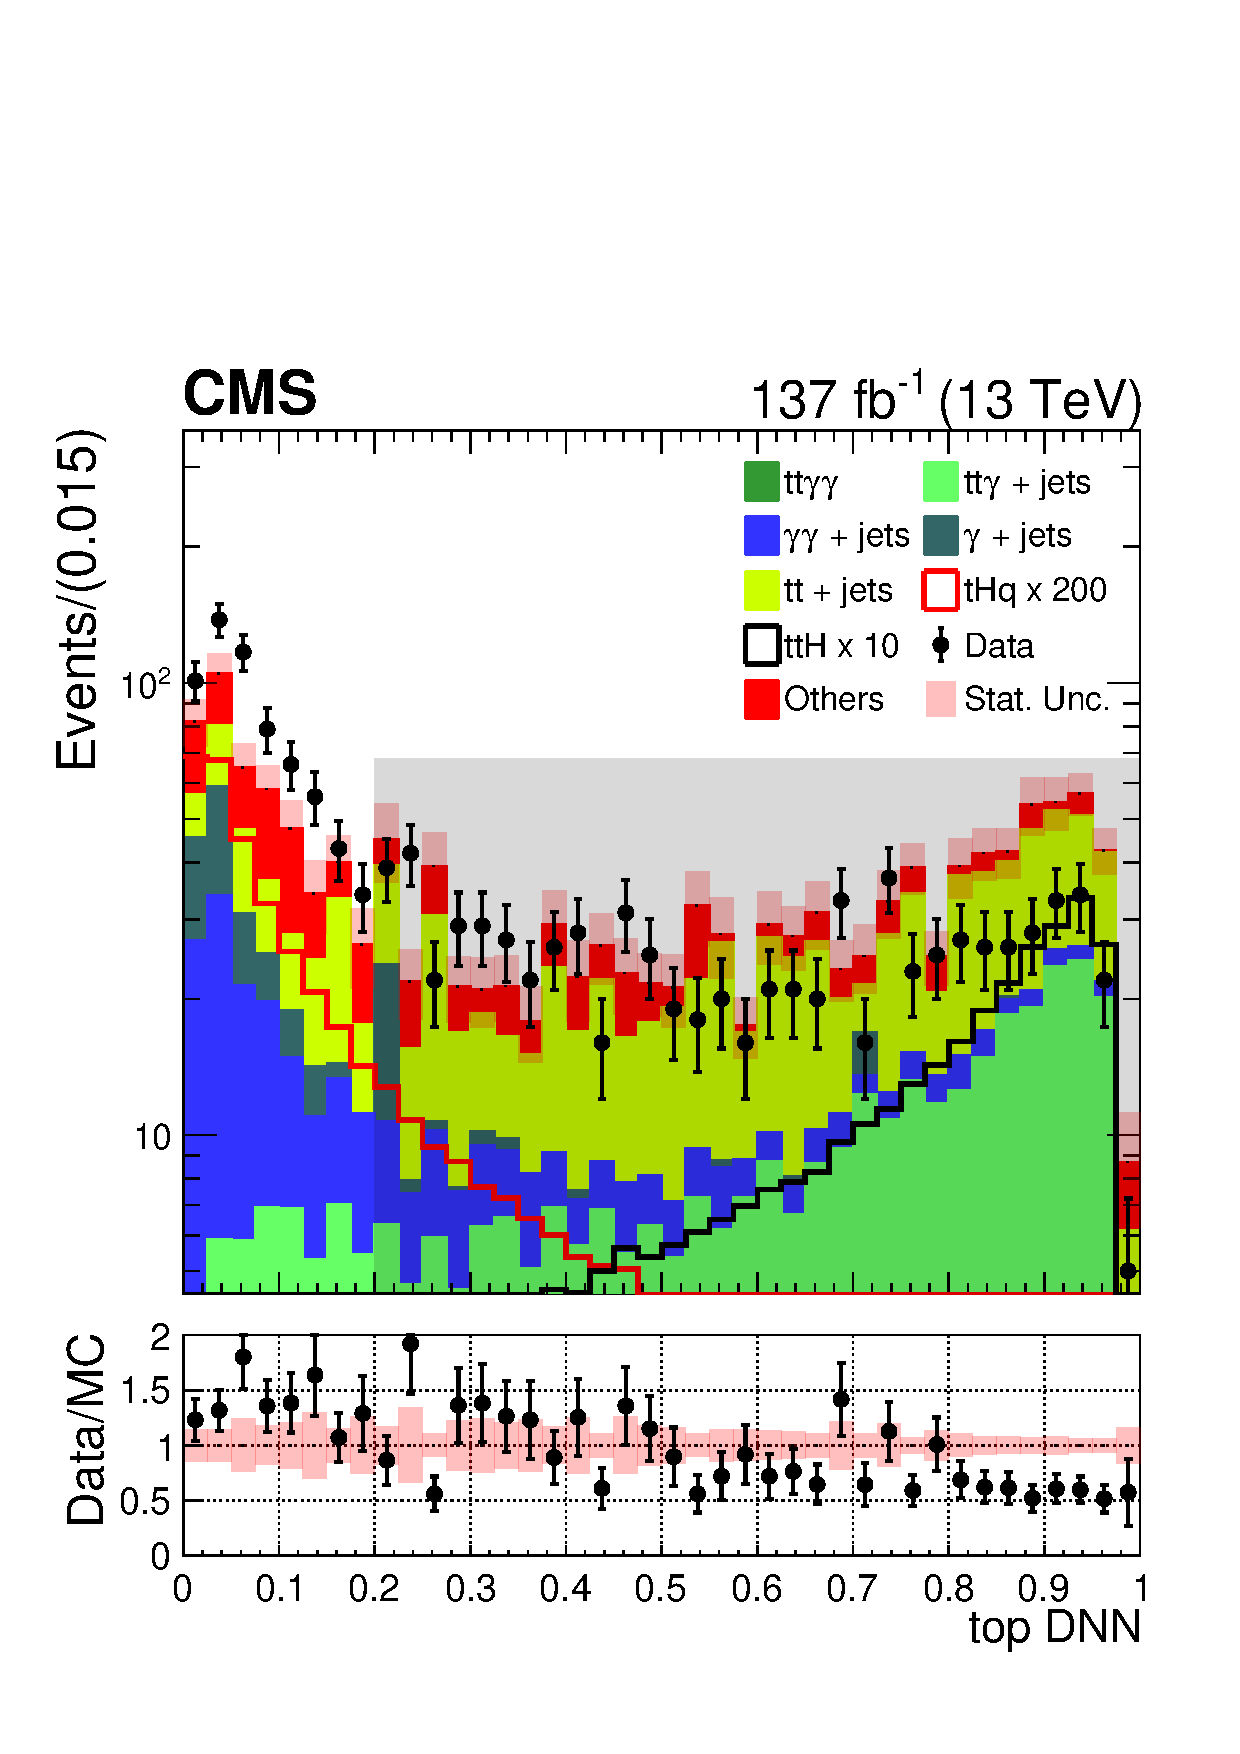
\includegraphics[width=.49\textwidth]{Figures/hgg_overview/tHq_DNN_score.pdf}
  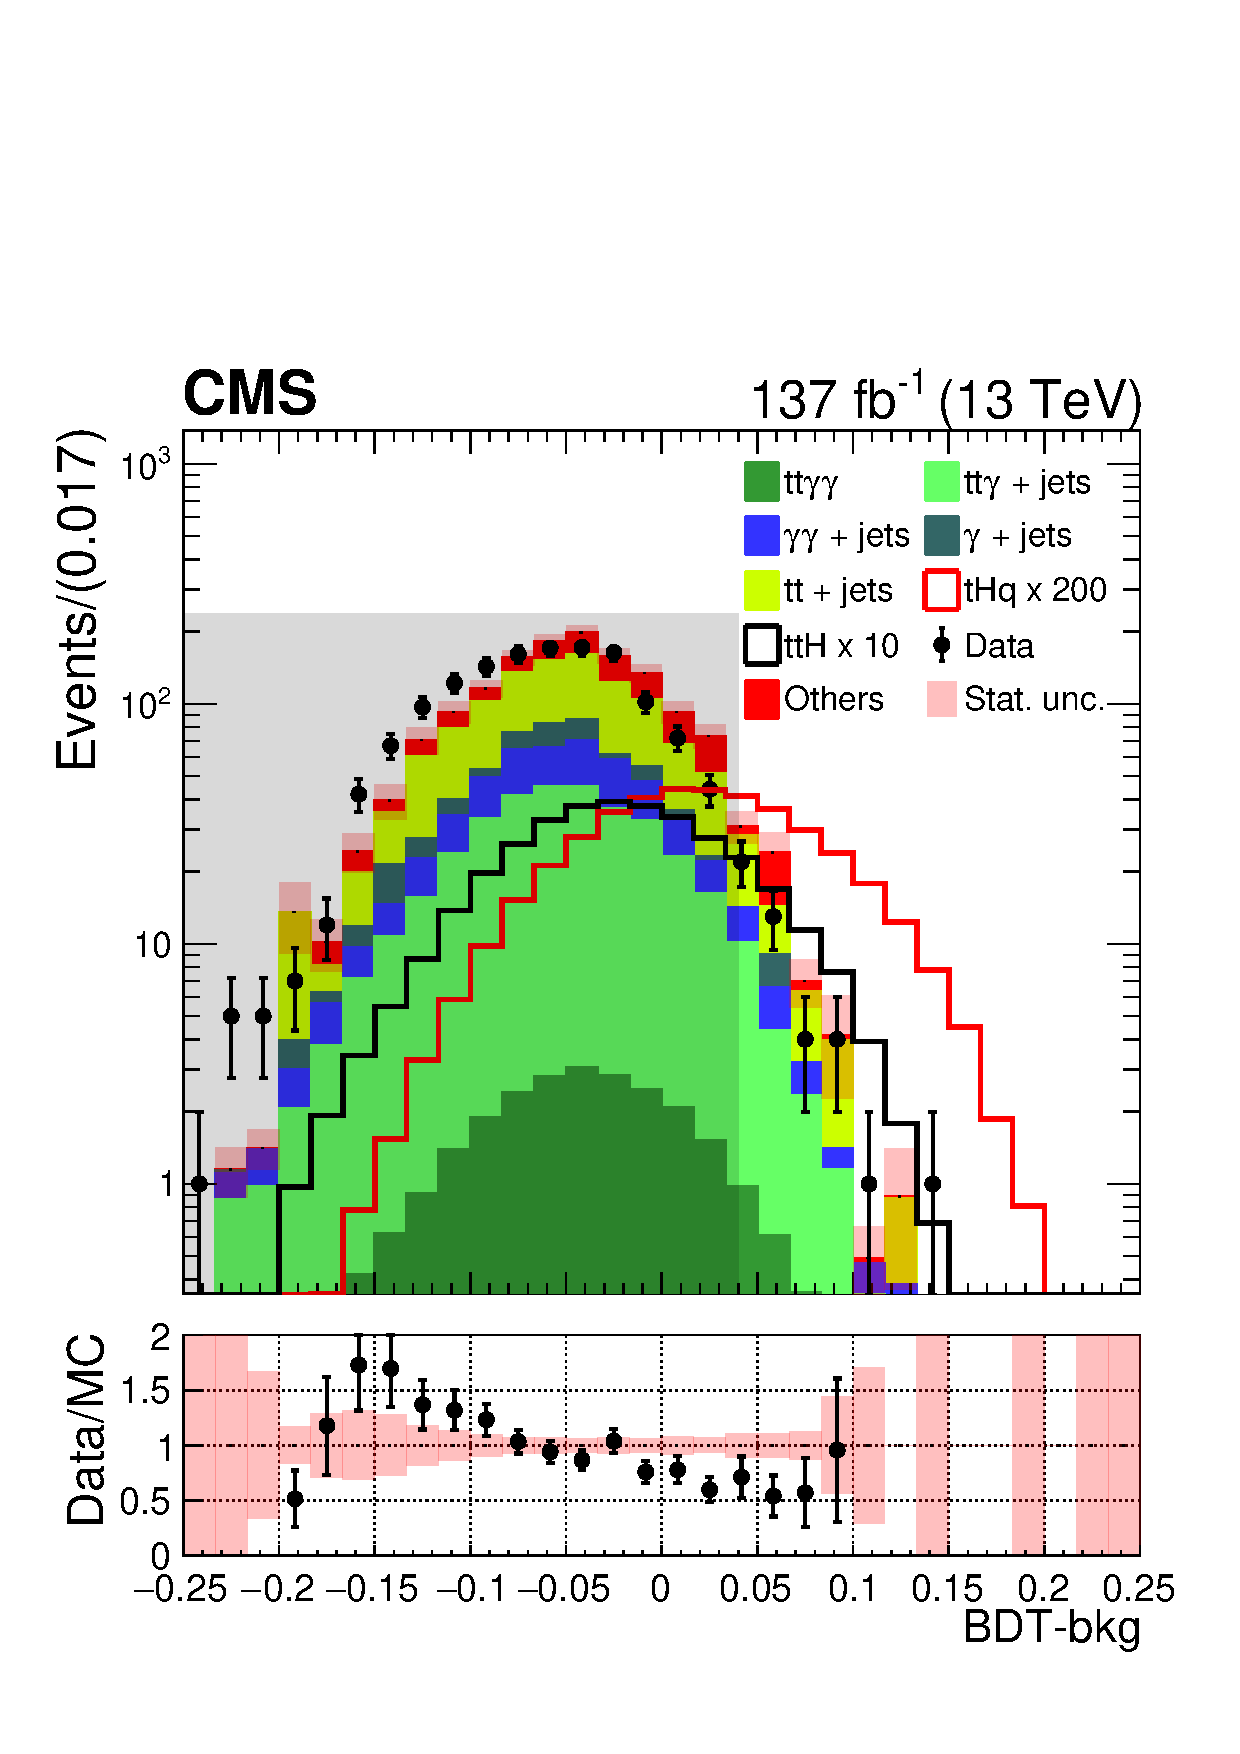
\includegraphics[width=.49\textwidth]{Figures/hgg_overview/tHq_BDT_score.pdf}
  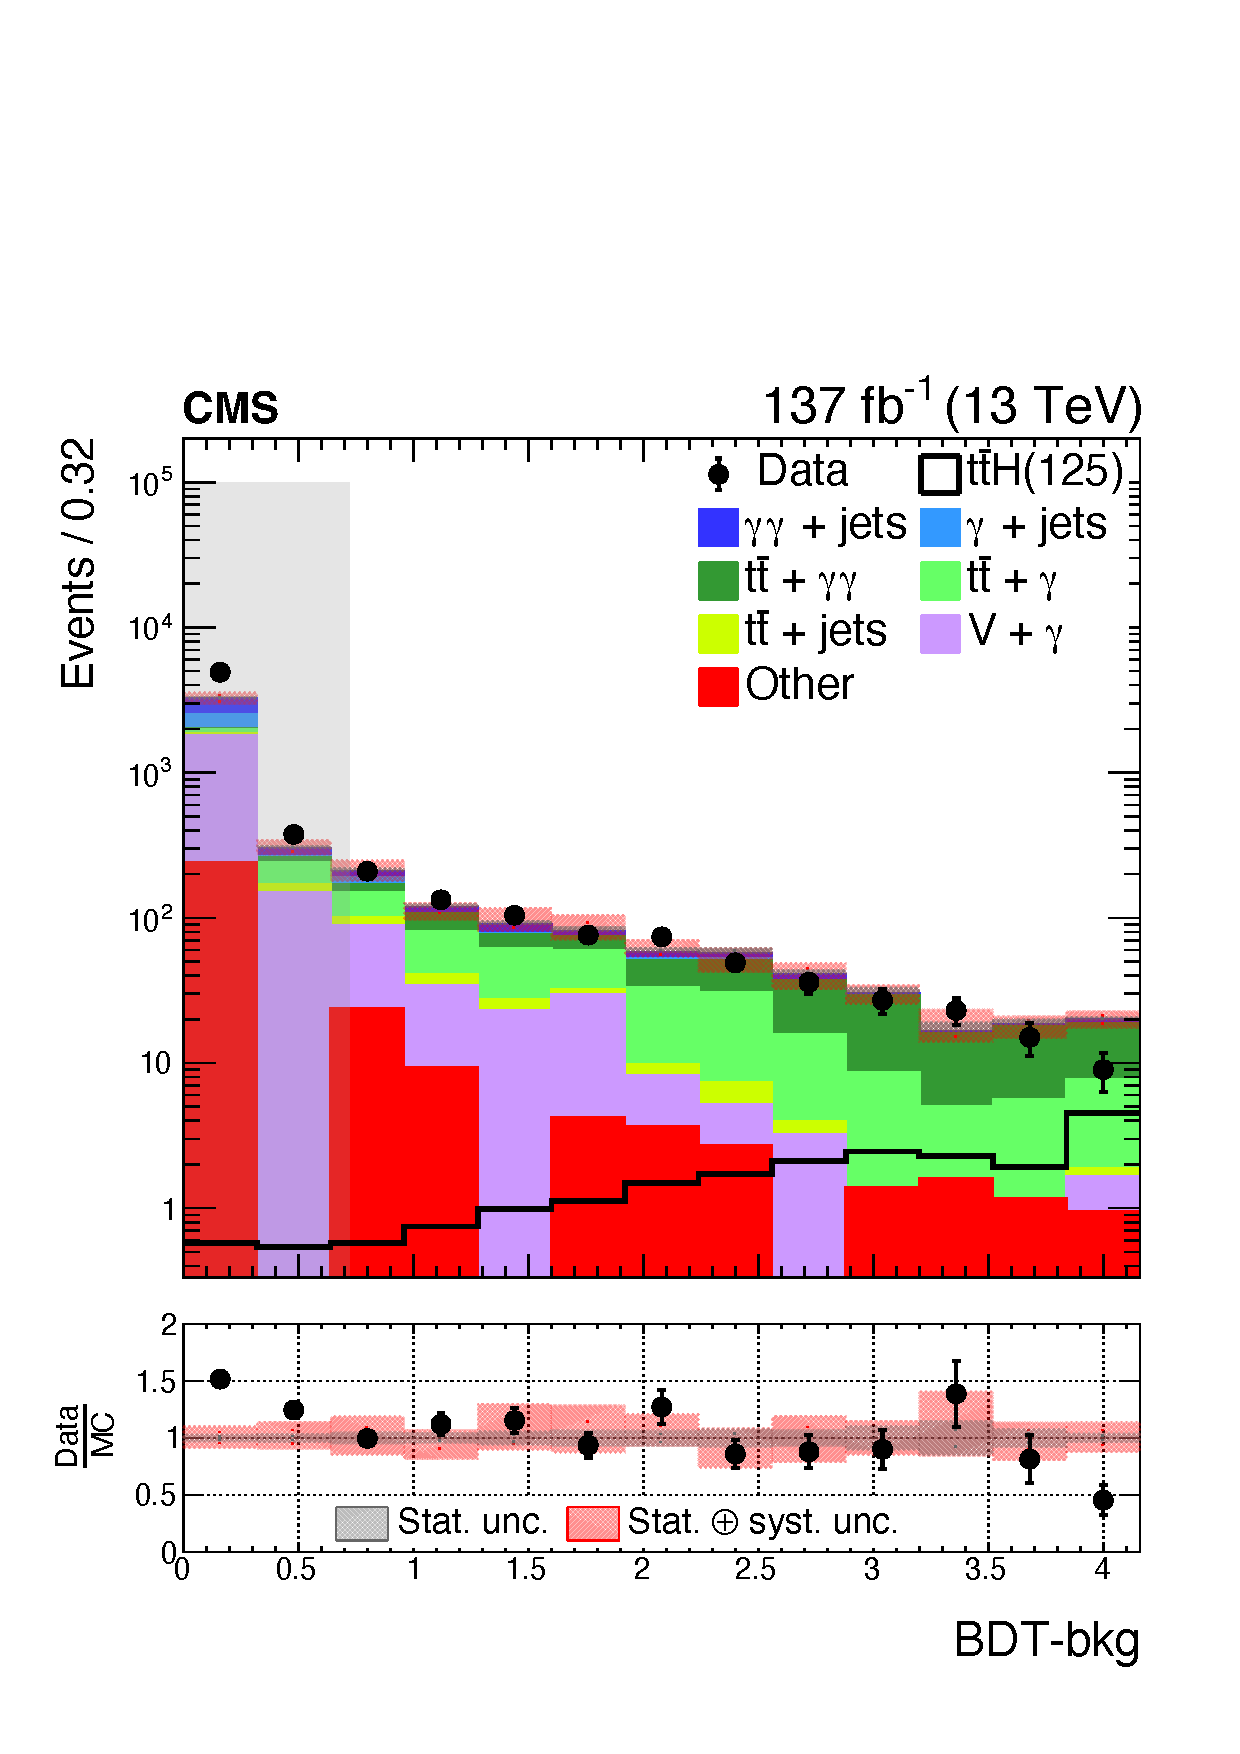
\includegraphics[width=.49\textwidth]{Figures/hgg_overview/ttHLeptonic_MVA.pdf}
  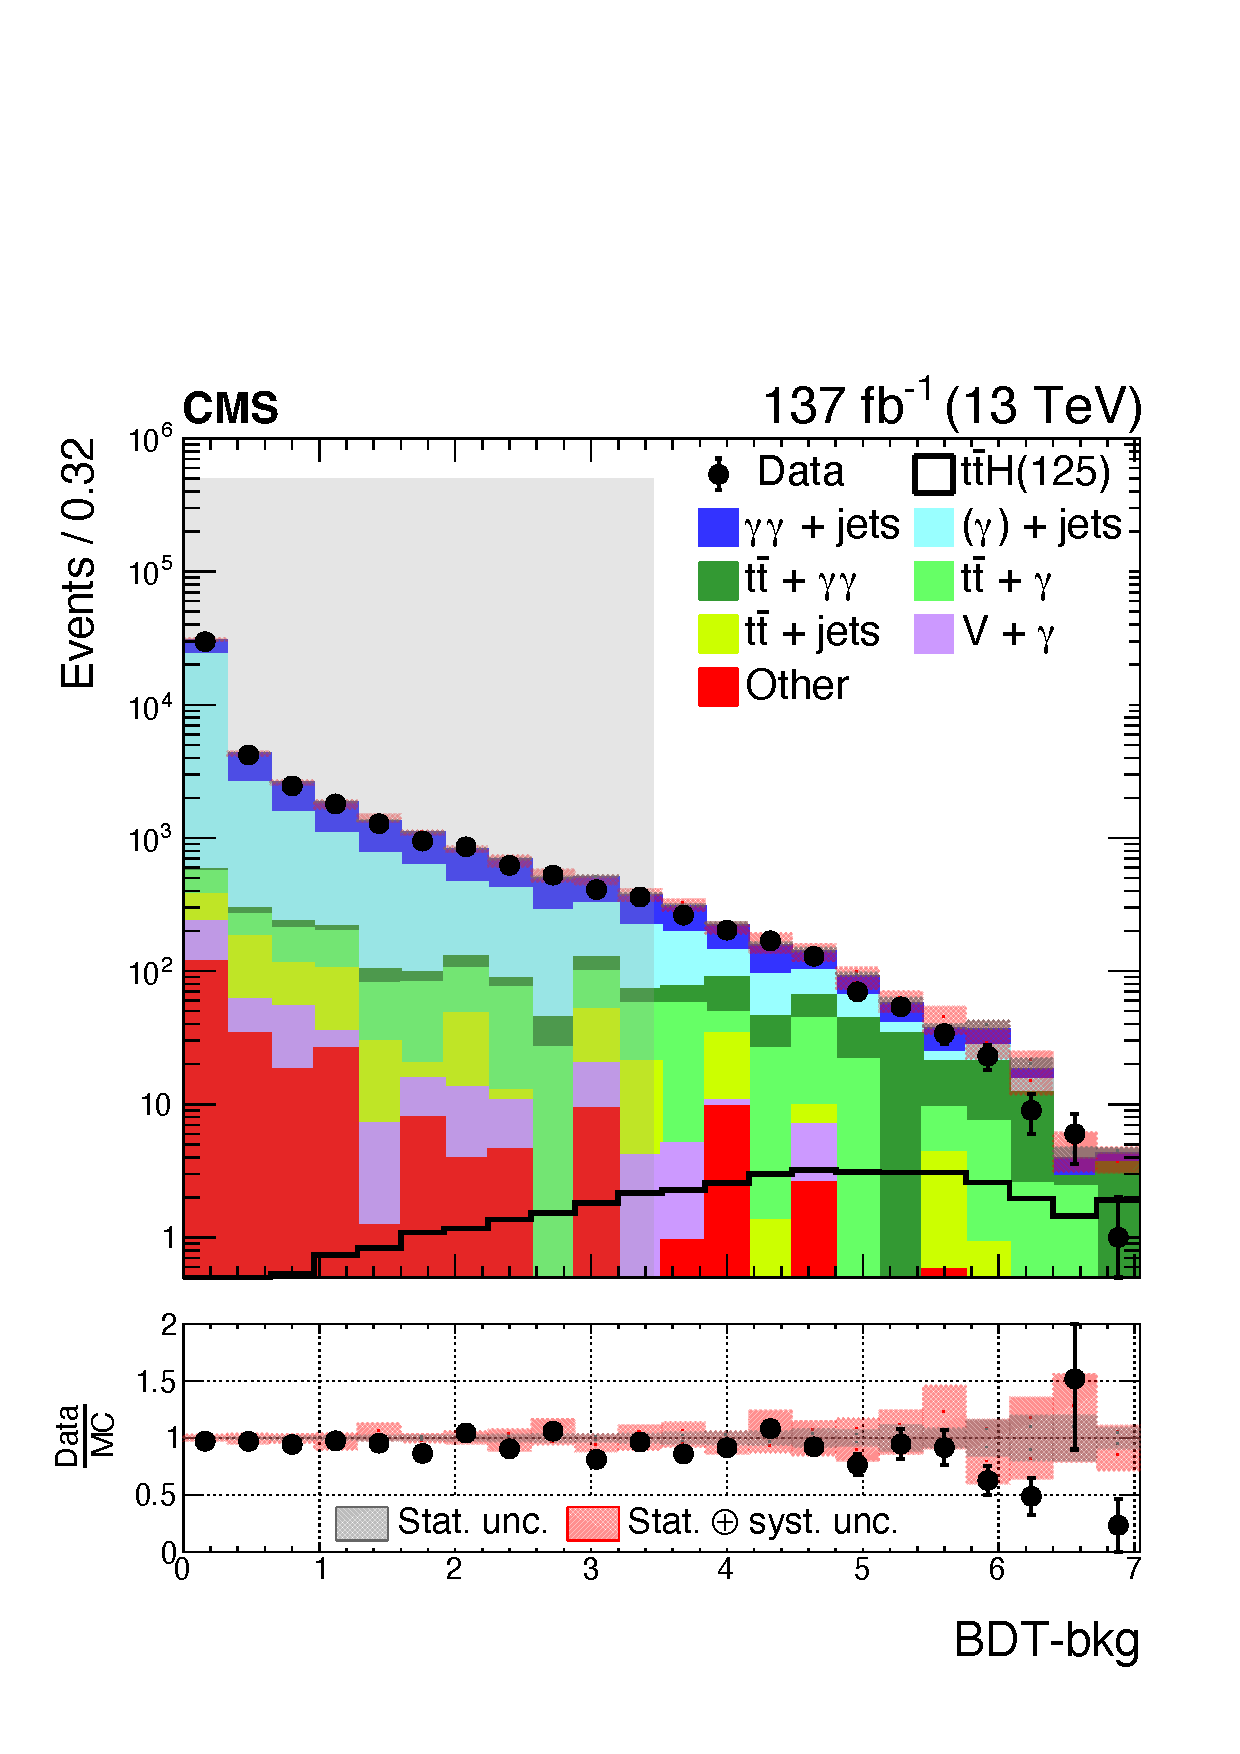
\includegraphics[width=.49\textwidth]{Figures/hgg_overview/ttHHadronic_MVA.pdf}
  \caption[Output scores of the discriminants used for the top-associated production mode categories]
  {
    Distributions of the Top DNN (top left), tHq leptonic BDT (top right), ttH leptonic BDT (bottom left), and  ttH hadronic BDT (bottom right) output scores, for both data and simulated signal and background events. The data events are taken from the \mgg sidebands: $[100,120]\cup[130,180]$~GeV. The statistical (statistical~$\oplus$~systematic) component of the uncertainty in the background estimate is shown by the red shaded band in the top two (bottom two) score distributions. The grey shaded region for the Top DNN score indicates the upper threshold for the tHq leptonic category. For the other output scores, the shaded regions illustrate the lowest threshold, beyond which events are not considered for the corresponding analysis categories. The full data set collected in the period 2016-2018 and the corresponding simulation is shown.
  }
  \label{fig:categorisation_top}
\end{figure}

\begin{table}
    \caption[Expected yields for the top-associated production mode categories]{The expected number of events for $m_{\rm{H}}=125$~GeV in the analysis categories targeting the top-associated production modes, shown for an integrated luminosity of 137~\fbinv. The fraction of the total number of events arising from each production mode in each analysis category is provided, as is the fraction of events originating from the targeted STXS bin (or bins). Here, ggH includes contributions from the sub-dominant ggZ(q$\bar{\rm{q}}$)H and bbH production modes, and qqH includes both VBF and V(q$\bar{\rm{q}}$)H production. The $\sigma_{\rm{eff}}$, defined as the smallest interval containing 68.3\% of the $m_{\gamma\gamma}$ distribution provides an indication of the mass resolution in each category. Also provided are the estimated number of background events-per-GeV in the signal peak region, the quantity $F_{68}=S_{68}/(S_{68}+B_{68})$, where $S_{68}$ and $B_{68}$ are the expected number of signal and background events in a $\pm1\sigma_{\rm{eff}}$ window centred on $m_{\rm{H}}$, respectively, and the approximate significance, $Z_{68}=S_{68}/\sqrt{S_{68}+B_{68}}$. The final column shows the significance for the targeted STXS bin (or bins) only, $Z^{\rm{target}}_{68}$,  where other Higgs boson signal events are considered as background.}
    \label{tab:top_category_yields}
    % \vspace{.5cm}
    \centering
    \scriptsize
    \renewcommand{\arraystretch}{1.2}
    \setlength{\tabcolsep}{3pt}
    \hspace*{-1.5cm}
    \begin{tabular}{l|ccccccccc|c|ccc}
    \multirow{3}{*}{Analysis categories} & \multicolumn{9}{c|}{SM 125 GeV Higgs boson expected signal} & \multirow{3}{*}{\begin{tabular}[c]{@{}c@{}}Bkg\\(GeV$^{\rm{-1}}$)\end{tabular}} & \multirow{3}{*}{$F_{68}$} & \multirow{3}{*}{$Z_{68}$} & \multirow{3}{*}{$Z^{\rm{target}}_{68}$} \\
     & \multirow{2}{*}{\begin{tabular}[c]{@{}c@{}}Total\\Yield\end{tabular}} & \multirow{2}{*}{\begin{tabular}[c]{@{}c@{}}Target\\Fraction\end{tabular}} & \multicolumn{6}{c}{Production Mode Fractions} & \multirow{2}{*}{\begin{tabular}[c]{@{}c@{}}$\sigma_{\rm{eff}}$\\(GeV)\end{tabular}} & & & & \\
     & & & ggH & qqH & VH lep & ttH & tHq & tHW & & & & & \\ \hline
     tHq lep & 1.8 & 23.9\% & 3.5\% & 3.7\% & 34.0\% & 28.8\% & 23.9\% & 6.0\% & 1.62 & 1.1 & 0.40 & 0.70 & 0.17 \\
     [\cmsTabSkip]
     ttH lep $\ptgg<60$ Tag0 & 0.8 & 93.8\% & - & - & 0.7\% & 98.2\% & 0.7\% & 0.5\% & 1.71 & 0.19 & 0.63 & 0.58 & 0.55 \\
     ttH lep $\ptgg<60$ Tag1 & 1.0 & 94.4\% & 0.0\% & - & 0.5\% & 97.9\% & 1.5\% & 0.7\% & 1.69 & 0.38 & 0.51 & 0.58 & 0.55 \\
     ttH lep $\ptgg<60$ Tag2 & 1.8 & 87.7\% & 0.0\% & 0.5\% & 5.1\% & 90.7\% & 3.2\% & 1.1\% & 1.94 & 3.0 & 0.17 & 0.46 & 0.40 \\
     [\cmsTabSkip]
     ttH lep $60<\ptgg<120$ Tag0 & 1.4 & 95.0\% & 0.0\% & 0.0\% & 1.0\% & 97.3\% & 1.0\% & 0.8\% & 1.60 & 0.34 & 0.64 & 0.78 & 0.75 \\
     ttH lep $60<\ptgg<120$ Tag1 & 0.6 & 90.8\% & 0.0\% & 0.7\% & 1.0\% & 95.6\% & 1.6\% & 1.1\% & 1.61 & 0.21 & 0.55 & 0.49 & 0.44 \\
     ttH lep $60<\ptgg<120$ Tag2 & 2.1 & 90.9\% & 0.0\% & 0.1\% & 2.8\% & 93.7\% & 2.5\% & 1.3\% & 1.92 & 1.2 & 0.39 & 0.74 & 0.67 \\
     [\cmsTabSkip]
     ttH lep $120<\ptgg<200$ Tag0 & 3.6 & 90.1\% & 0.3\% & 0.2\% & 2.7\% & 92.8\% & 2.0\% & 2.0\% & 1.63 & 0.59 & 0.71 & 1.31 & 1.18 \\
     ttH lep $120<\ptgg<200$ Tag1 & 0.8 & 77.9\% & 2.0\% & 0.5\% & 11.3\% & 80.6\% & 3.2\% & 2.5\% & 1.72 & 0.44 & 0.43 & 0.50 & 0.39 \\
     [\cmsTabSkip]
     ttH lep $200<\ptgg<300$ Tag0 & 2.5 & 85.9\% & 0.1\% & 0.0\% & 4.1\% & 88.1\% & 3.0\% & 4.8\% & 1.54 & 0.51 & 0.68 & 1.08 & 0.93 \\
     [\cmsTabSkip]
     ttH lep $\ptgg>300$ Tag0 & 2.1 & 61.7\% & 1.0\% & 0.0\% & 18.0\% & 69.3\% & 3.0\% & 8.7\% & 1.57 & 0.53 & 0.64 & 0.96 & 0.59 \\
     [\cmsTabSkip]
     ttH had $\ptgg<60$ Tag0 & 1.2 & 94.2\% & 1.7\% & 0.2\% & 0.0\% & 96.6\% & 0.9\% & 0.4\% & 1.68 & 0.50 & 0.49 & 0.64 & 0.60 \\
     ttH had $\ptgg<60$ Tag1 & 0.4 & 93.5\% & 0.1\% & 0.9\% & 0.0\% & 96.7\% & 1.7\% & 0.6\% & 1.66 & 0.26 & 0.38 & 0.31 & 0.29 \\
     ttH had $\ptgg<60$ Tag2 & 3.1 & 89.8\% & 1.6\% & 1.5\% & 0.3\% & 92.9\% & 3.0\% & 0.7\% & 1.88 & 6.6 & 0.14 & 0.54 & 0.49 \\
     [\cmsTabSkip]
     ttH had $60<\ptgg<120$ Tag0 & 1.8 & 92.6\% & 0.6\% & 0.0\% & 0.1\% & 97.6\% & 1.1\% & 0.6\% & 1.55 & 0.24 & 0.77 & 0.97 & 0.90 \\
     ttH had $60<\ptgg<120$ Tag1 & 0.4 & 90.8\% & 4.6\% & 0.8\% & 0.0\% & 91.9\% & 1.9\% & 0.8\% & 1.35 & 0.33 & 0.39 & 0.33 & 0.30 \\
     ttH had $60<\ptgg<120$ Tag2 & 5.2 & 88.7\% & 1.0\% & 2.2\% & 0.5\% & 91.8\% & 3.5\% & 1.0\% & 1.90 & 6.6 & 0.22 & 0.88 & 0.78 \\
     [\cmsTabSkip]
     ttH had $120<\ptgg<200$ Tag0 & 3.6 & 91.4\% & 1.5\% & 0.4\% & 0.1\% & 94.7\% & 2.2\% & 1.3\% & 1.53 & 0.87 & 0.65 & 1.25 & 1.14 \\
     ttH had $120<\ptgg<200$ Tag1 & 2.1 & 83.3\% & 4.6\% & 2.9\% & 0.5\% & 86.2\% & 4.2\% & 1.7\% & 1.76 & 1.3 & 0.38 & 0.74 & 0.61 \\
     ttH had $120<\ptgg<200$ Tag2 & 1.7 & 74.3\% & 10.0\% & 4.6\% & 0.6\% & 76.5\% & 6.3\% & 2.0\% & 1.65 & 1.9 & 0.26 & 0.55 & 0.41 \\
     ttH had $120<\ptgg<200$ Tag3 & 2.6 & 62.2\% & 15.4\% & 8.4\% & 1.2\% & 64.7\% & 8.5\% & 1.9\% & 1.73 & 6.6 & 0.13 & 0.49 & 0.30 \\
     [\cmsTabSkip]
     ttH had $200<\ptgg<300$ Tag0 & 2.0 & 90.1\% & 0.5\% & 0.4\% & 0.1\% & 92.3\% & 3.8\% & 2.9\% & 1.44 & 0.37 & 0.72 & 1.00 & 0.90 \\
     ttH had $200<\ptgg<300$ Tag1 & 1.5 & 74.6\% & 8.8\% & 3.1\% & 0.7\% & 77.0\% & 6.8\% & 3.5\% & 1.47 & 0.59 & 0.54 & 0.74 & 0.55 \\
     ttH had $200<\ptgg<300$ Tag2 & 1.7 & 56.5\% & 18.8\% & 8.4\% & 0.4\% & 58.0\% & 10.5\% & 3.8\% & 1.59 & 1.8 & 0.30 & 0.59 & 0.33 \\
     [\cmsTabSkip]
     ttH had $\ptgg>300$ Tag0 & 2.5 & 73.8\% & 8.3\% & 1.6\% & 0.8\% & 74.9\% & 7.7\% & 6.8\% & 1.44 & 0.39 & 0.75 & 1.13 & 0.84 \\
     ttH had $\ptgg>300$ Tag1 & 1.9 & 45.6\% & 27.1\% & 7.3\% & 1.4\% & 46.0\% & 11.4\% & 6.7\% & 1.56 & 0.74 & 0.52 & 0.82 & 0.37 \\
     [\cmsTabSkip]
\end{tabular}
    \hspace*{-1.5cm}
\end{table}

% \FloatBarrier

\subsection{Validation}\label{sec:cat_validation}
It is necessary to validate the modelling of the large number of ML classifiers used in this analysis. In this context, validation means requiring a good agreement between data and MC simulation in the outputs of the numerous classifiers, particularly in the signal-like regions where events enter the analysis. 

In Sections~\ref{sec:ggh_categorisation}--\ref{sec:top_categorisation}, the output-score distributions of all ML classifiers used in the event categorisation are shown for simulated signal and background events (used to train the ML classifiers), and for the corresponding data which can be compared to the simulated background. A good agreement here gives confidence that the background processes are accurately modelled, and therefore that the ML algorithm performs well in the classification task. Since the background model used in the final results extraction is derived directly from data, poor agreement in the background-like regions cannot introduce bias, but will only lead to a sub-optimal performance of the ML classifier. 

A second form of validation is used for the signal-like regions. This involves finding an independent sample of events with signal-like characteristics and comparing the output score of the ML classifiers in both data and simulation. Since the signal model is derived from simulation, a disagreement in the classifier output may introduce a systematic uncertainty into the signal estimate. Therefore, we require a good agreement between data and simulation, within the statistical and systematic uncertainties in the MC, to instil confidence that the simulated signal events are sufficiently well-modelled.

The plots in Figure \ref{fig:categorisation_validation} show the validation of the ggH BDT, the diphoton BDT, the dijet BDT (via $p_{\rm{VBF}}$), and the VH hadronic BDT, all using \Zee events in simulation and data. The uncertainty band on the simulation demonstrates the addition in quadrature of the statistical and systematic components, where the systematic component includes uncertainties originating from the photon-ID BDT, photon-energy resolution, and the jet-energy scale and resolution (see Section \ref{sec:systematics}). The ggH BDT distribution shows the number of events attributed to each output class. It can be seen that there is an excellent agreement between data and simulation, well within uncertainties, particularly in the signal regions which enter the analysis categories. All in all, this means the included systematic uncertainties in the signal estimates are sufficient to cover the discrepancies in the output classifier scores, and no additional sources of systematic uncertainty are required. 

Figure~\ref{fig:top_validation} shows the equivalent plots for the ttH leptonic BDT and ttH hadronic BDT classifiers; here ttZ, \Zee events are used for the validation as they share similar kinematic properties with the targeted ttH signal process. Again, good agreement is observed between data and simulation, particularly in the signal-like regions with high BDT output score.

\begin{figure}
  \centering
  \hfill
  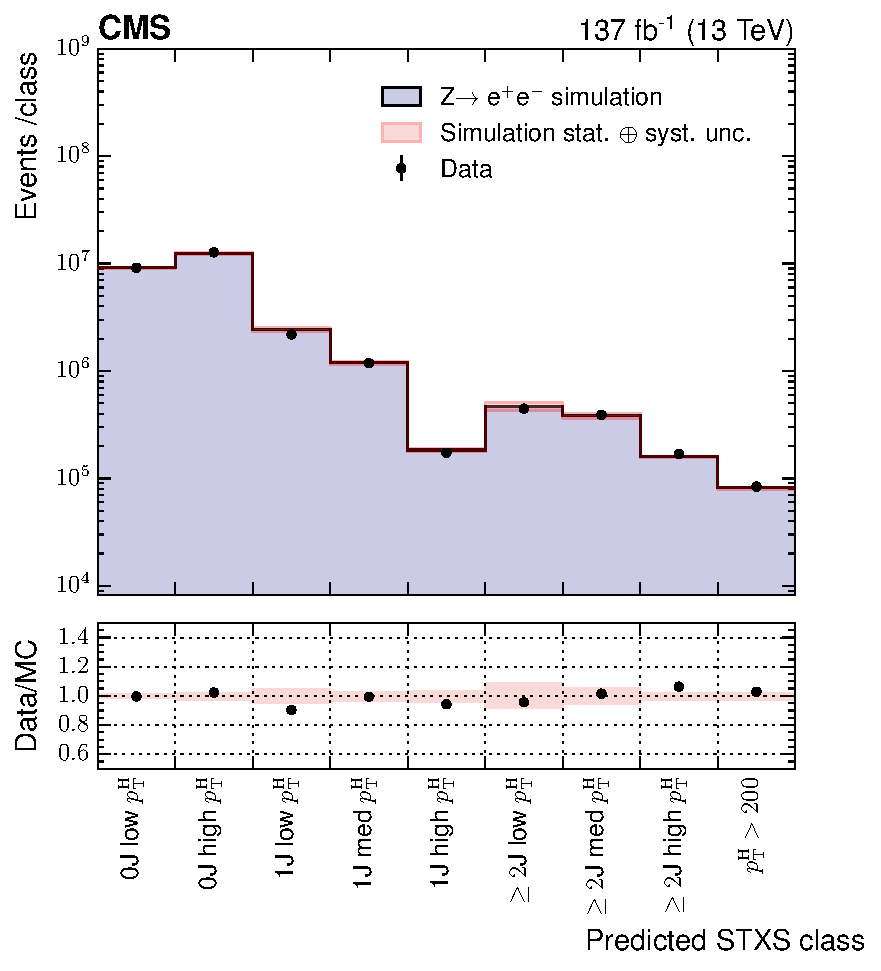
\includegraphics[height=7.25cm]{Figures/hgg_overview/DYValidation_ggH_argmax_ratioPlot_logPlot.pdf}
  \hfill
  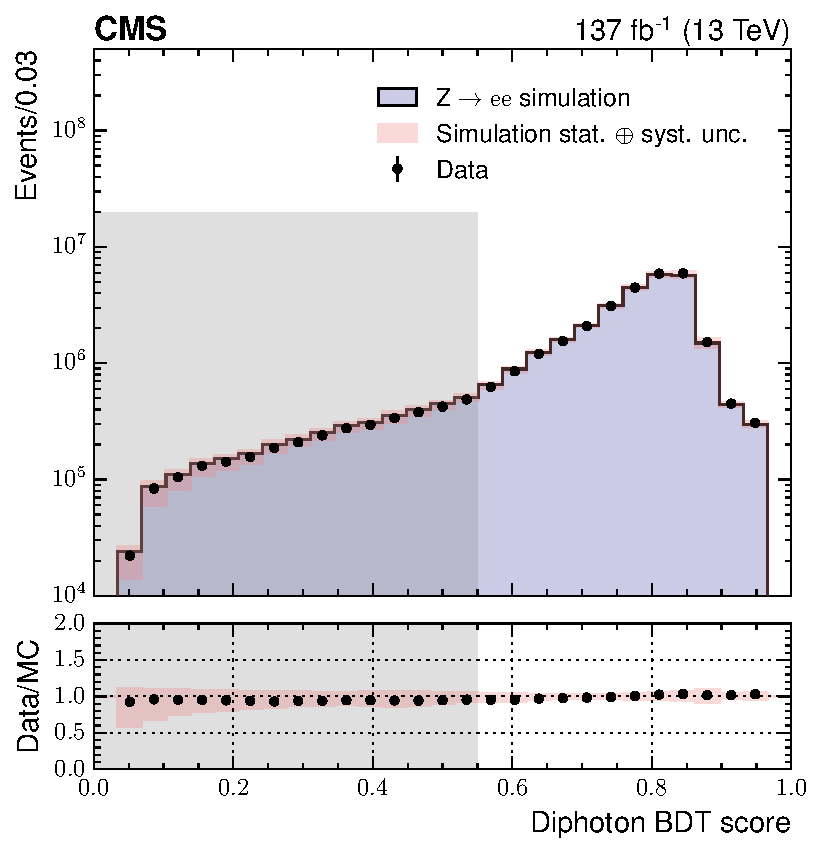
\includegraphics[height=7.25cm]{Figures/hgg_overview/DYValidation_DiphoBDT_ratioPlot_dipho_mva_logPlot.pdf}
%   \vspace{-.5cm}
%   \vspace{1cm}
  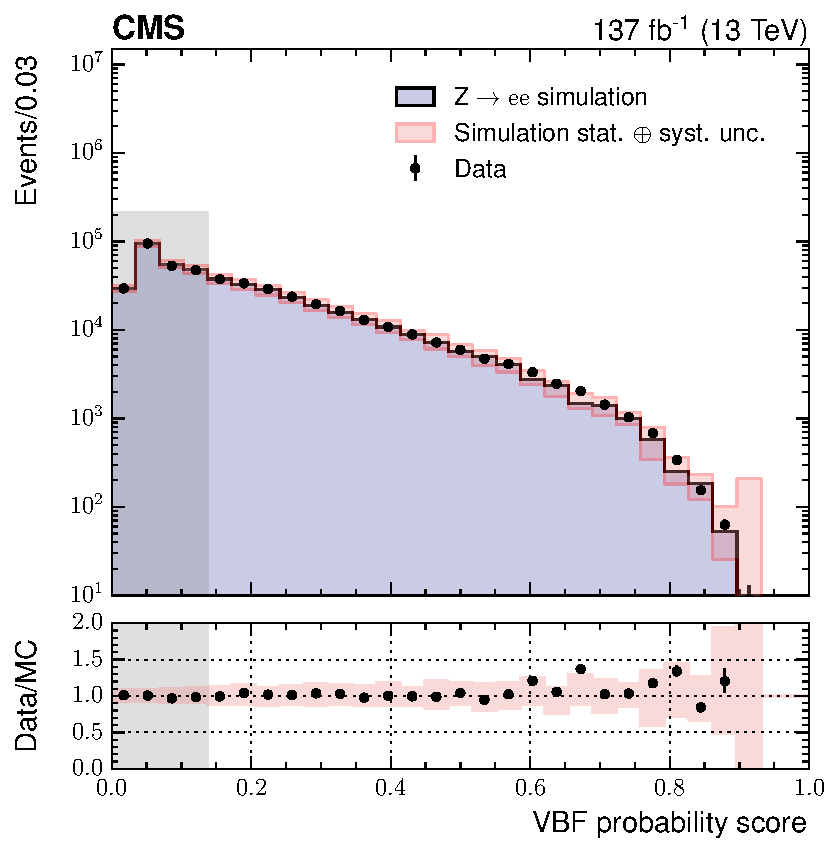
\includegraphics[height=7.25cm]{Figures/hgg_overview/DYValidation_VBFBDT_ratioPlot_vbfMvaResult_prob_VBF_logPlot.pdf}
  \hfill
  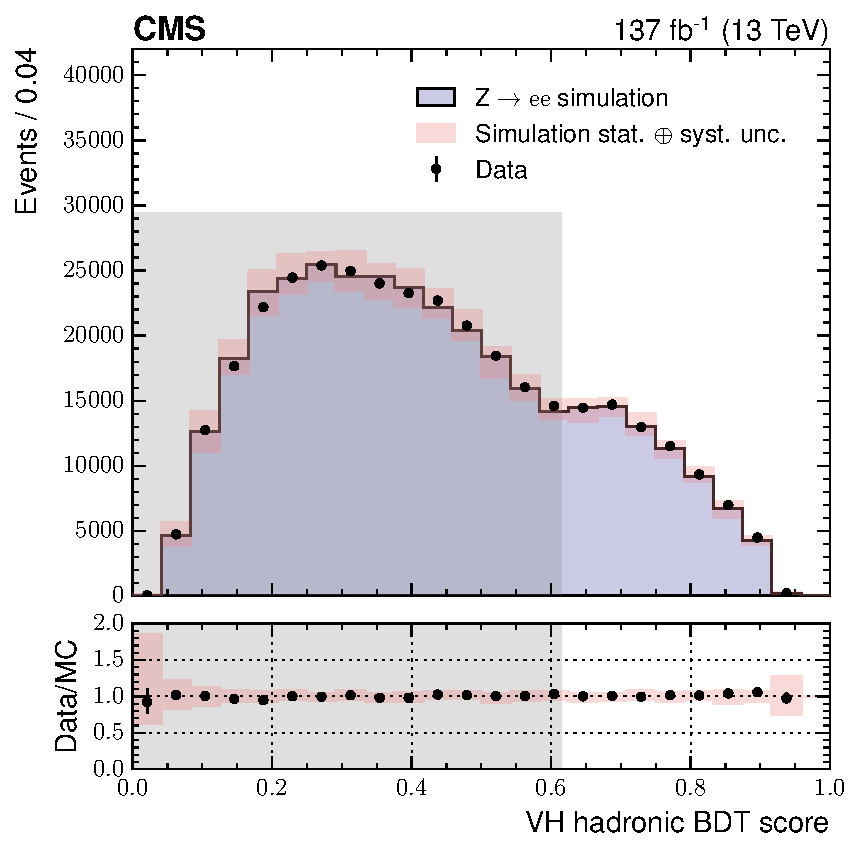
\includegraphics[height=7.25cm]{Figures/hgg_overview/DYValidation_VHBDT_VH_had_mvascore_ratioPlot.pdf}
  \caption[Validation of the event categorisation classifiers]
  {
    The validation of the ggH BDT (top left), diphoton BDT (top right), dijet BDT via $p_{\rm{VBF}}$ (bottom left) and the VH hadronic BDT (bottom right), where the distribution of the outputs are shown for \Zee events in data (black points) and simulation (filled histogram). The pink bands represent the quadrature sum of the statistical and systematic uncertainties in the simulated events. The regions shaded grey show the thresholds in the scores, below which no events enter the relevant analysis categories.
  }
  \label{fig:categorisation_validation}
\end{figure}

\begin{figure}
  \centering
  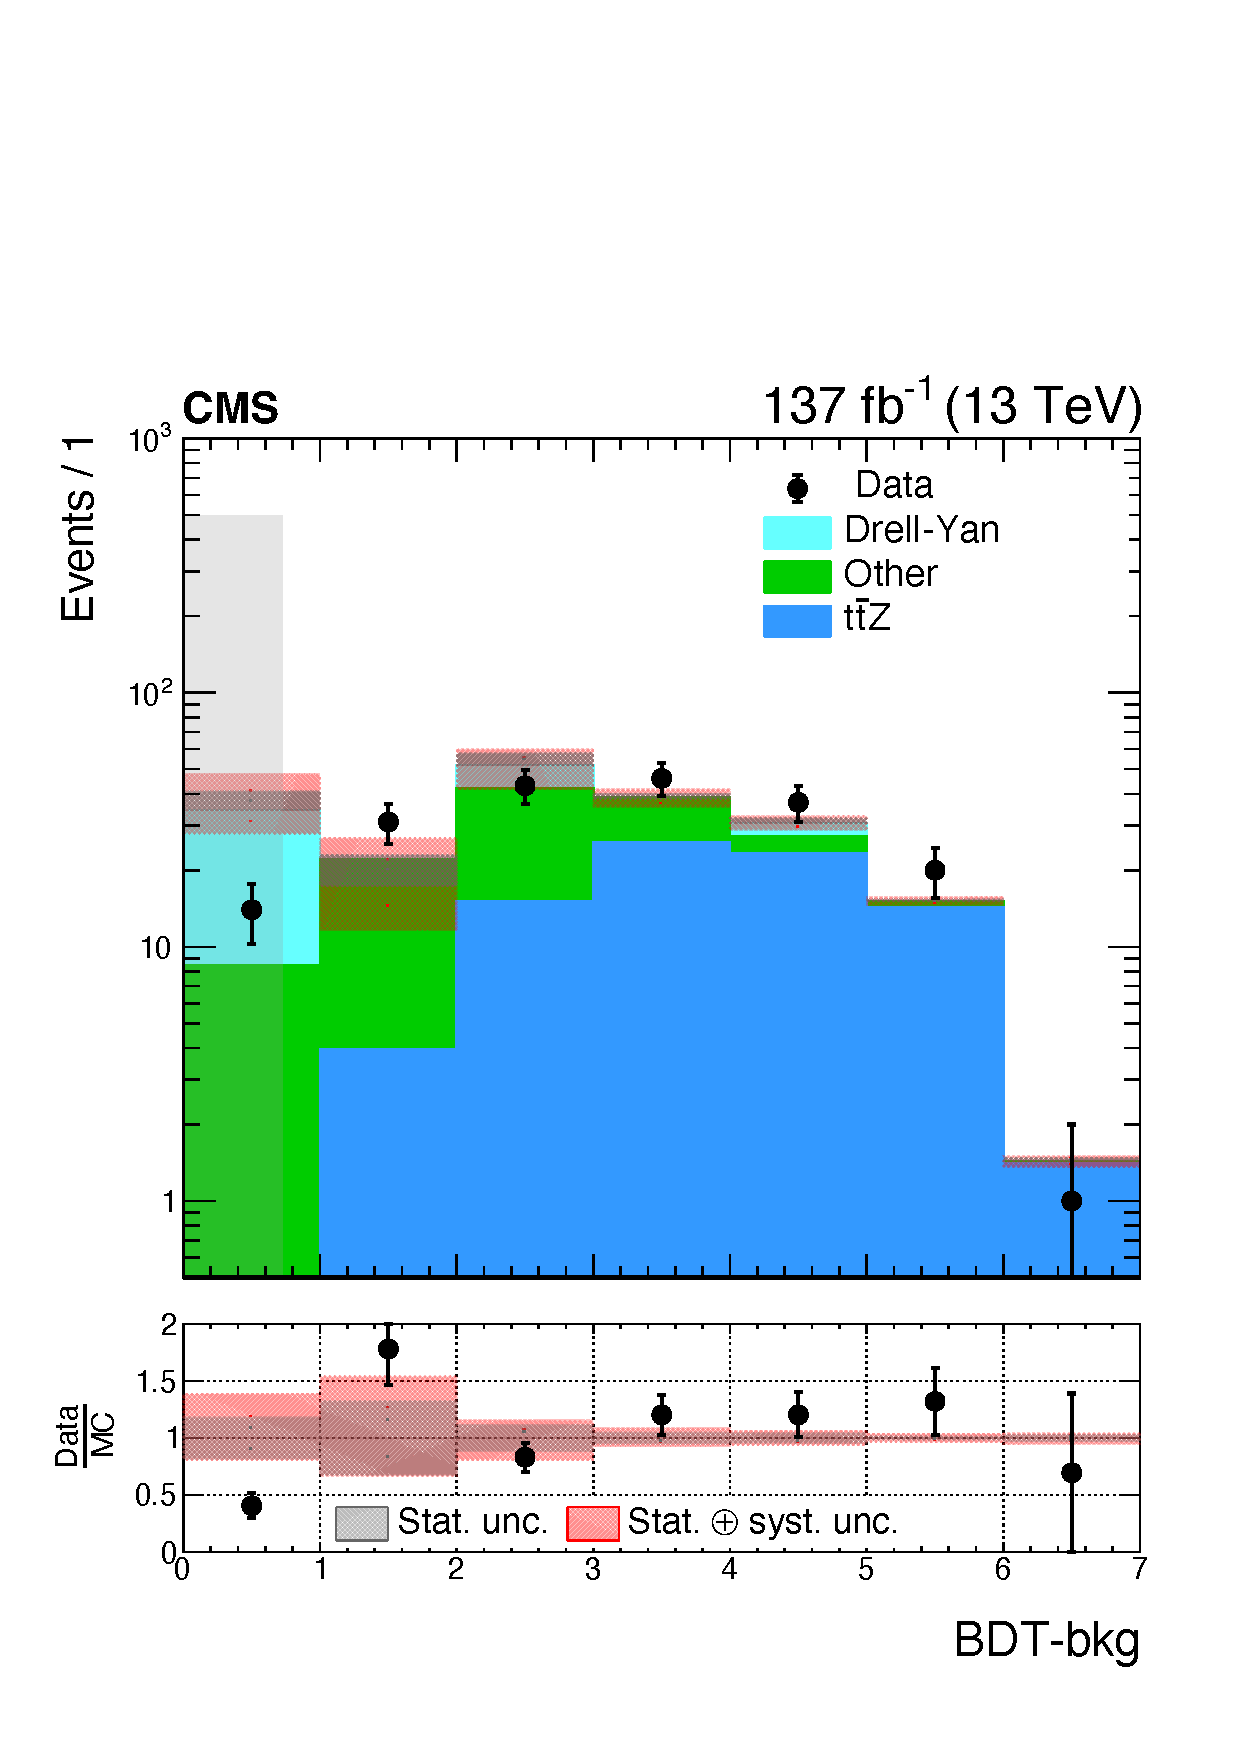
\includegraphics[width=.49\textwidth]{Figures/hgg_overview/ttHLeptonic_MVA_ttZ.pdf}
  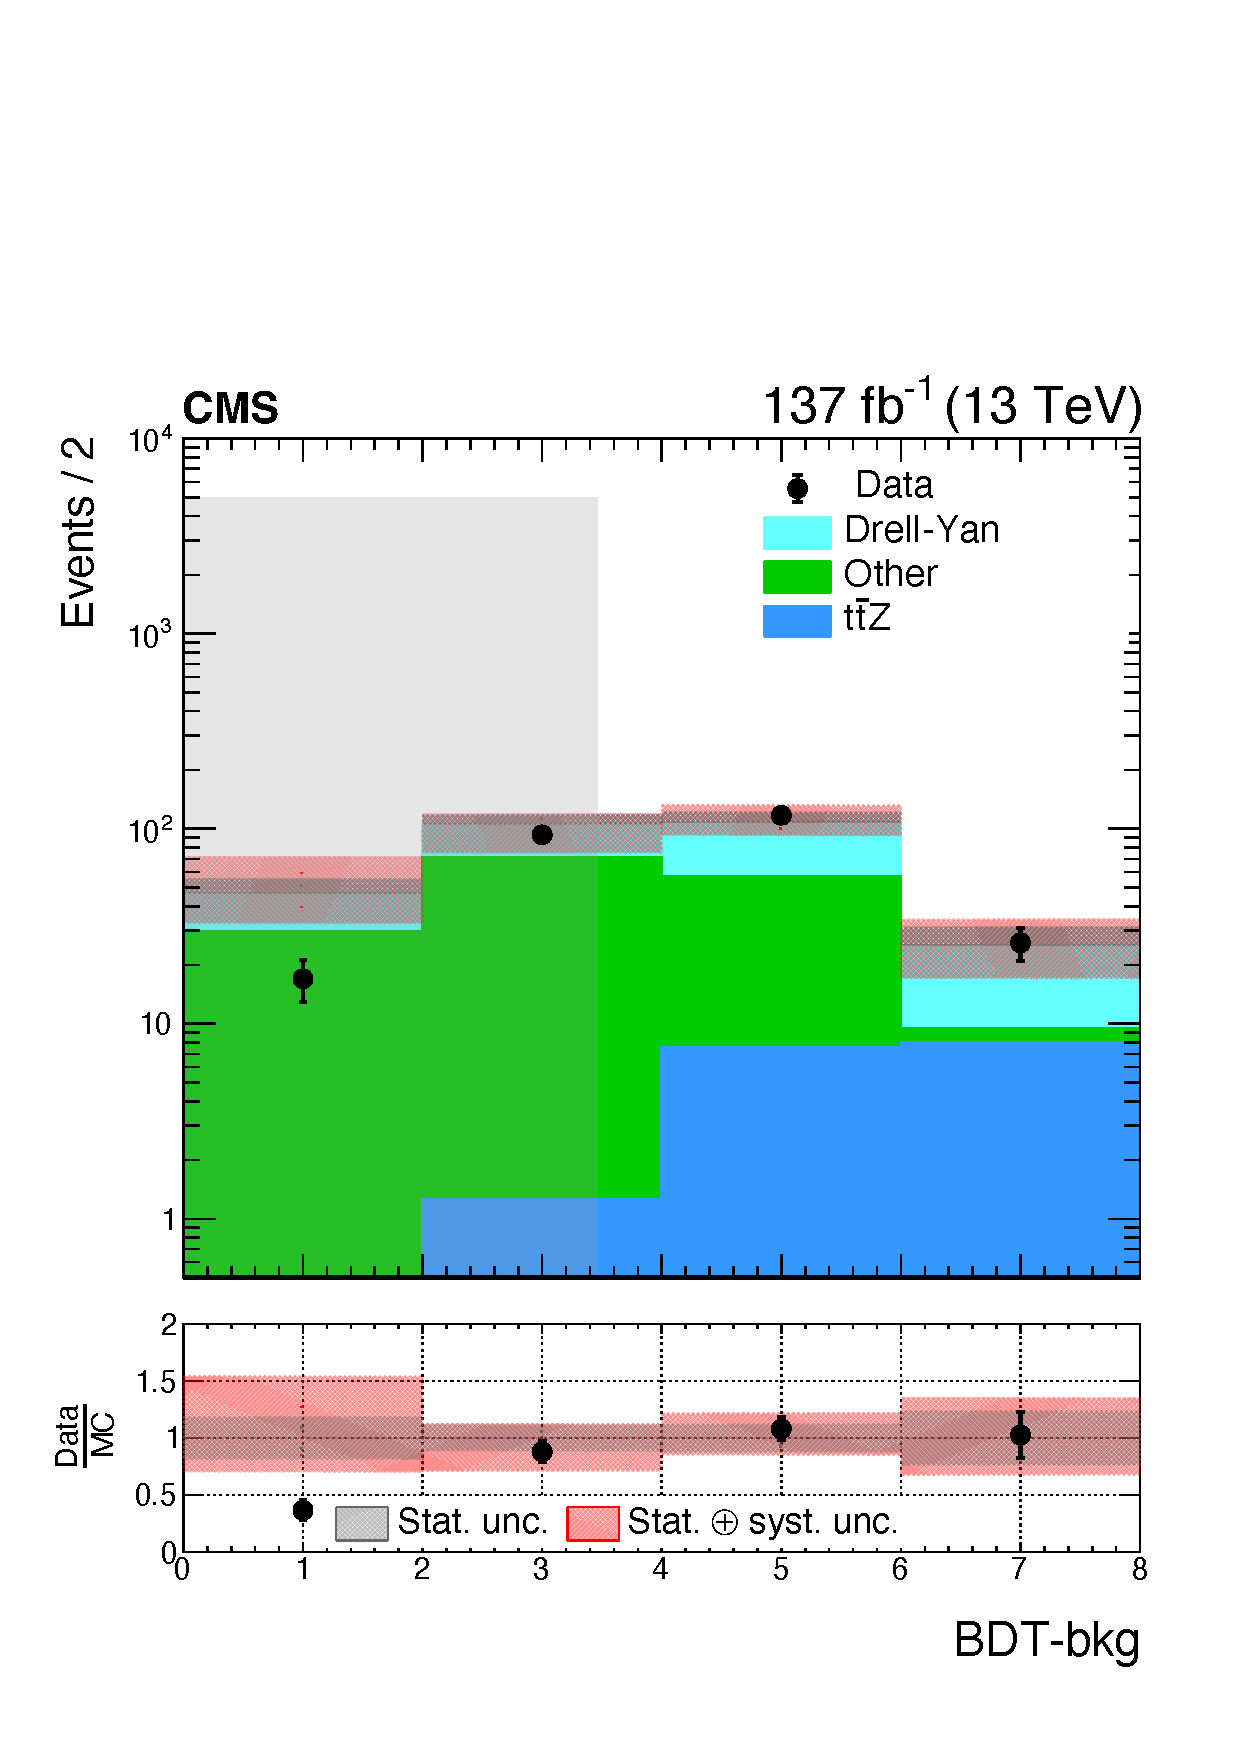
\includegraphics[width=.49\textwidth]{Figures/hgg_overview/ttHHadronic_MVA_ttZ.pdf}
  \caption[Validation of the top-associated classifiers]
  {
    The validation of the ttH leptonic BDT (left) and ttH hadronic BDT (right) classifiers, where the distribution of the outputs are shown for ttZ events in data (black points) and simulation (filled histogram). The ttZ events are required to pass the same initial selection criteria for the corresponding global category, with additional requirements on the dielectron kinematics, number of jets, and number of b tagged jets to increase the ttZ purity. The pink (black) bands represent the quadrature sum of the statistical and systematic uncertainties (statistical uncertainty only) in the simulated background events. The shaded-grey regions indicate the scores which do not enter the relevant analysis categories.
  }
  \label{fig:top_validation}
\end{figure}

% \FloatBarrier
%%%%%%%%%%%%%%%%%%%%%%%%%%%%%%%%%%%%%%%%%%%%%%%%%%%%%%%%%%%%%%%%%%%%%%%%%%%%%%%%%%%%%%%%%%%%%%%%
% \newpage
\section{Summary}

This chapter has described the selection, reconstruction and subsequent categorisation of p-p collision events recorded by the CMS detector in order to measure Higgs boson production cross sections and couplings in the \Hgg decay channel. The confusion matrix in Figure \ref{fig:purity_matrix} displays the expected signal-composition of the final \textit{reconstruction-level} analysis categories in terms of the \textit{truth-level} STXS bins. In the plot, the analysis categories targeting a common STXS region (tags) are summed, such that the signal compositions of the individual analysis categories are weighted according to $F_{68}=S_{68}/(S_{68}+B_{68})$. The numbers in the matrix represent the fractional contribution of the total signal yield in a given analysis category group arising from each STXS bin, such that each row sums to 100\%. Ultimately, by making this matrix as diagonal as possible, we improve the sensitivity to the individual STXS regions, and reduce the correlations between the measured quantities. The full unweighted confusion matrix, split into the individual analysis categories, is provided in Appendix~\ref{app:eff_acc}.

\begin{figure}
  \centering
  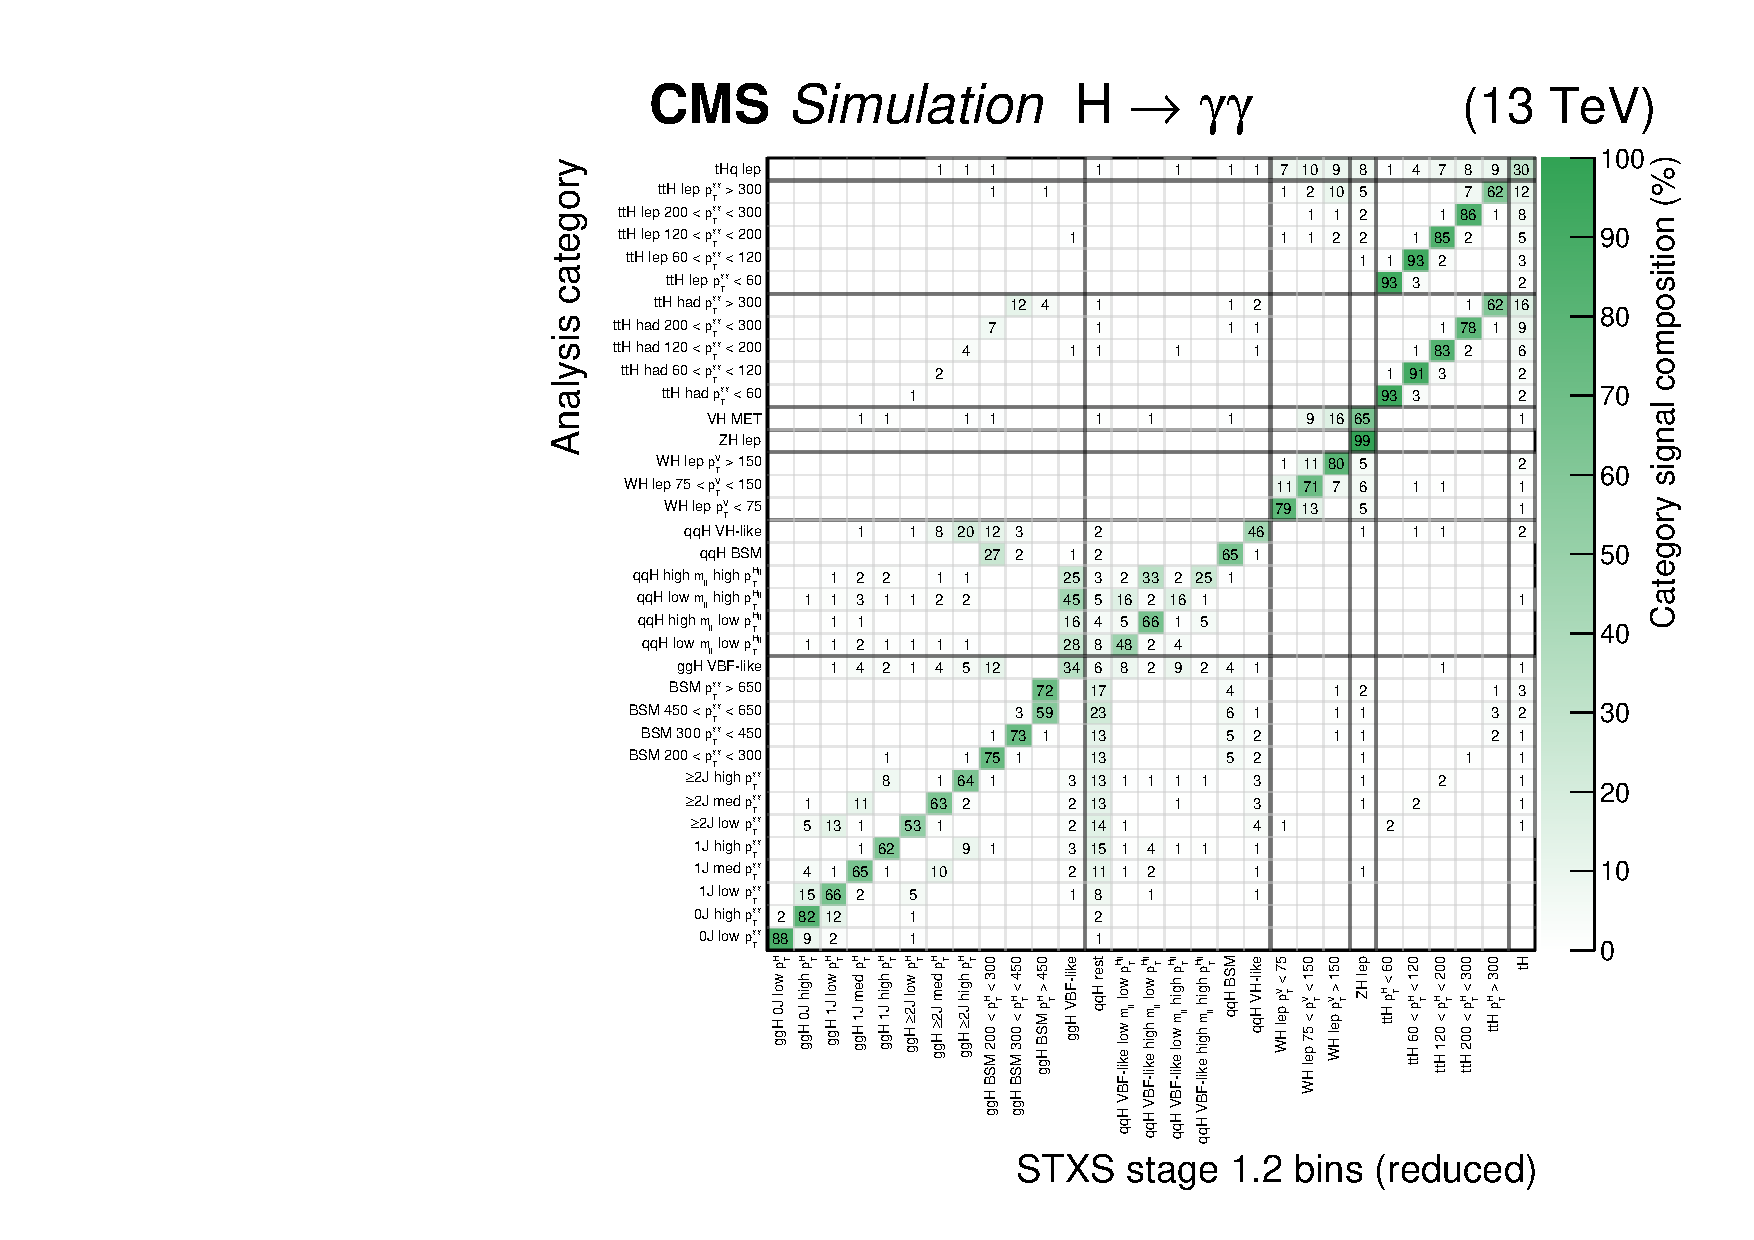
\includegraphics[width=.95\textwidth]{Figures/hgg_overview/purityMatrix_merged.pdf}
  \caption[Confusion matrix for the analysis categories]
  {
    Confusion matrix displaying the composition of the analysis categories in terms of a merged set of STXS bins. The granularity of the STXS bin merging corresponds to the finest granularity used for the cross section measurements. Analysis categories targeting a common STXS region are summed, where the signal compositions of the individual analysis categories are weighted in the sum by $F_{68}=S_{68}/(S_{68}+B_{68})$. The colour scale indicates the fractional yield in each analysis category group (rows) accounted for by each STXS process (columns). Each row therefore sums to 100\%. Entries with values less than 0.5\% are not shown. Simulated events for each year in the period 2016-2018 are combined with appropriate weights corresponding to their relative integrated luminosity in data. The column labelled as qqH rest includes the contributions from the qqH 0J, qqH 1J, qqH $m_{jj}<60$~GeV and the qqH $120<m_{jj}<350$~GeV STXS bins.
  }
  \label{fig:purity_matrix}
\end{figure}

The next chapter explains the procedure for unfolding this matrix by fitting the diphoton mass distributions in each analysis category, in order to extract the measurements of the truth-level production cross sections and other parameters of interest.






